\documentclass{article}
\usepackage[top=1in, bottom=1in, left=1in, right=1in]{geometry}
\usepackage[subpreambles=true]{standalone}
\usepackage[utf8]{inputenc}
\usepackage[english]{babel}
\usepackage{import}
\usepackage{hyperref}
\usepackage[]{multibib}
\usepackage{float}
\usepackage{caption}
\usepackage{subcaption}
\usepackage{graphicx}
\usepackage{xcolor}
\usepackage{rotating}
\usepackage{tikz}
\usetikzlibrary{arrows,shapes,positioning,shadows,trees}
\usetikzlibrary{arrows.meta}
\usepackage{nomencl}
\usepackage{amsmath}
\usepackage{color,soul}
\usepackage{listings}
\usepackage{dirtytalk}
\usepackage{csquotes}
\usepackage{imakeidx}
\makeindex[columns=3, title=Alphabetical Index, intoc]
\usepackage{cancel}
\usepackage{ulem}
\usepackage{algpseudocode}
\usepackage{algorithm}
\usepackage{pdfpages}
\usepackage{multirow}
\usepackage{multicol}
\providecommand{\tabularnewline}{\\}
\usepackage{amssymb}% http://ctan.org/pkg/amssymb
\usepackage{pifont}% http://ctan.org/pkg/pifont

\newcommand{\cmark}{\ding{51}}%
\newcommand{\xmark}{\ding{55}}%

\usepackage[breakable]{tcolorbox}
\usepackage{parskip} % Stop auto-indenting (to mimic markdown behaviour)  
% Maintain compatibility with old templates. Remove in nbconvert 6.0
\let\Oldincludegraphics\includegraphics

%\DeclareCaptionFormat{nocaption}{}
%\captionsetup{format=nocaption,aboveskip=0pt,belowskip=0pt}
\floatplacement{figure}{H} % forces figures to be placed at the correct location
\usepackage{enumerate} % Needed for markdown enumerations to work
\usepackage{textcomp} % defines textquotesingle

\definecolor{codegreen}{rgb}{0,0.6,0}
\definecolor{codegray}{rgb}{0.5,0.5,0.5}
\definecolor{codepurple}{rgb}{0.58,0,0.82}
\definecolor{backcolour}{rgb}{0.95,0.95,0.92}

\lstdefinestyle{mystyle}{
    backgroundcolor=\color{backcolour},   
    commentstyle=\color{codegreen},
    keywordstyle=\color{magenta},
    numberstyle=\tiny\color{codegray},
    stringstyle=\color{codepurple},
    basicstyle=\ttfamily\footnotesize,
    breakatwhitespace=false,         
    breaklines=true,                 
    captionpos=b,                    
    keepspaces=true,                 
    numbers=left,                    
    numbersep=5pt,                  
    showspaces=false,                
    showstringspaces=false,
    showtabs=false,                  
    tabsize=2
}

\lstset{style=mystyle}

\newcommand*{\DrawBoundingBox}[1][]{%
    \draw [red, very thick, #1]
    ([shift={(-5pt,-5pt)}]current bounding box.south west)
    rectangle
    ([shift={(5pt,+5pt)}]current bounding box.north east);
}

\title{DATA-DRIVEN TURBULENCE MODELING}
\author{Lorenzo Campoli}
\date{\today}

\begin{document}

\maketitle

\makenomenclature
% Nomenclature
\nomenclature{T}{Task}
\nomenclature{ST}{Subtask}
\nomenclature{Q}{Question}
\nomenclature{QoI}{Quantity of Interest}
\nomenclature{OF}{OpenFOAM}
\nomenclature{SCE}{Statistically Combined Ensemble}
\nomenclature{SOM}{Self-Organizing Map}
\nomenclature{ROI}{Region Of Interest}
\nomenclature{STL}{Standard Tessellation Language or STereoLithography}
\nomenclature{CSV}{Comma-Separated Values}
%
\nomenclature{b}{Prototype quality measures}
\nomenclature{$b_{ij}$,\textbf{b}}{Reynolds stress anisotropy tensor}
\nomenclature{$C_1$, $C_2$, $C_3$}{Barycentric map limiting state coordinates}
\nomenclature{$d_M$}{Mahalanobis distance}
\nomenclature{$f_x$}{Feature set, with case label $x$}
\nomenclature{$g_i$}{Coefficient in Pope tensor basis expansion}
\nomenclature{$\Bar{i}$}{Impurity}
\nomenclature{k}{Number of clusters}
\nomenclature{m}{Misclassification rate}
\nomenclature{$N_{proto}$}{Number of prototypes}
\nomenclature{P}{Turbulent production}
\nomenclature{$Re_{\tau}$}{Channel flow Reynolds number based on friction velocity and channel half-width}
\nomenclature{$S_{ij}$, \textbf{S}}{Mean strain rate tensor}
\nomenclature{$T_i$}{Pope tensor invariant}
\nomenclature{u}{Fraction of uncovered examples}
\nomenclature{$u^+$}{Mean velocity normalized by friction velocity}
\nomenclature{$W$}{Mean rotation rate tensor}
\nomenclature{$x_B$, $y_B$}{Barycentric map Cartesian coordinates}
\nomenclature{$y^+$}{Distance from wall normalized by viscous length scale}
\nomenclature{$\delta$}{Prototype algorithm sphere radius}
\nomenclature{$\varepsilon$}{Turbulent dissipation}
\nomenclature{$\eta_1$, $\eta_2$, ..., $\eta_5$}{Scalar invariants of Reynolds stress, strain, and rotation rate tensor combinations}
\nomenclature{$\theta$, $\varphi$, $\xi$}{Angles defining relative tensor or vector coordinate system orientations}
\nomenclature{$\kappa$, }{Eigenvalues of the Reynolds stress anisotropy tensor}
\nomenclature{$\lambda_1$, $\lambda_2$, ... , $\lambda_5$}{Pope scalar invariants}
\nomenclature{$\xi$}{Data set example}
\nomenclature{$\tau_{ij}$}{Reynolds stress tensor}
\nomenclature{$\chi$}{Prototype penalty parameter}
\nomenclature{$\omega_i$}{Mean vorticity vector}
\printnomenclature[3cm]

\tableofcontents

\listoffigures

\listoftables

%\chapter{The "selector"}
\section{Problem statement}
Let's consider, as concrete examples, a 3d hill geometry of Fig.~\ref{fig:examples}a or a submarine model with full appendages of Fig.~\ref{fig:examples}b.

\begin{figure}[H]%
    \centering
    \subfloat[\centering The (BeVERLI) hill geometry.]{{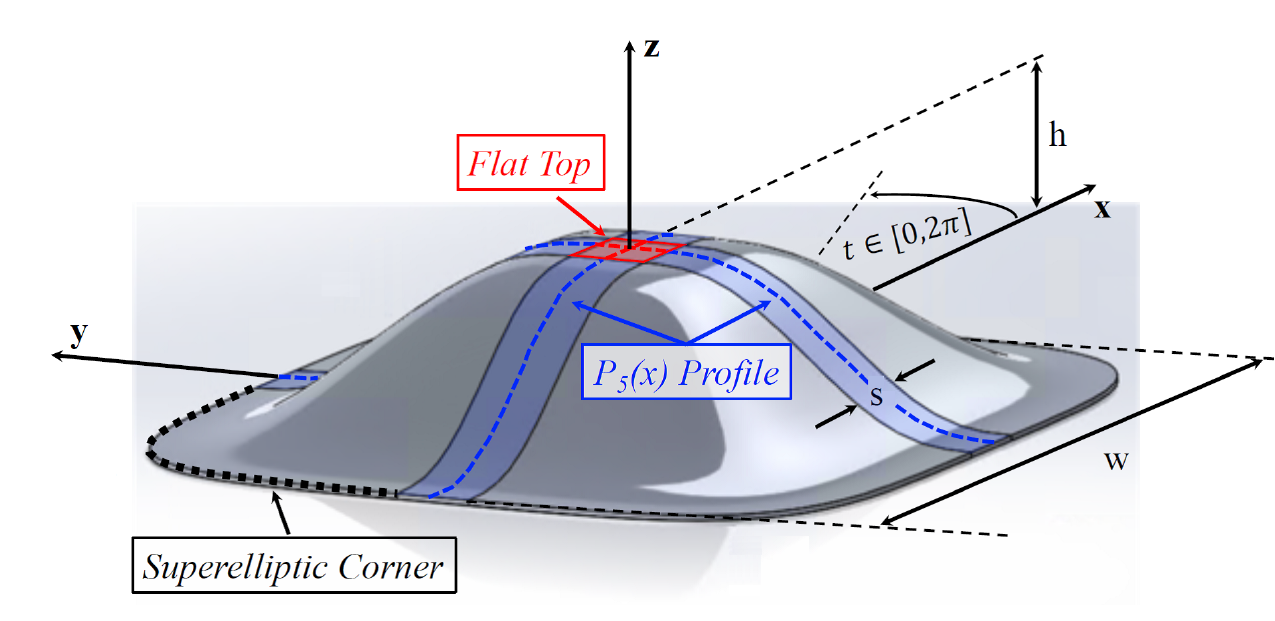
\includegraphics[width=0.45\textwidth]{figs/hill.png}}}%
    \qquad
    \subfloat[\centering A generic (BB2) submarine.]{{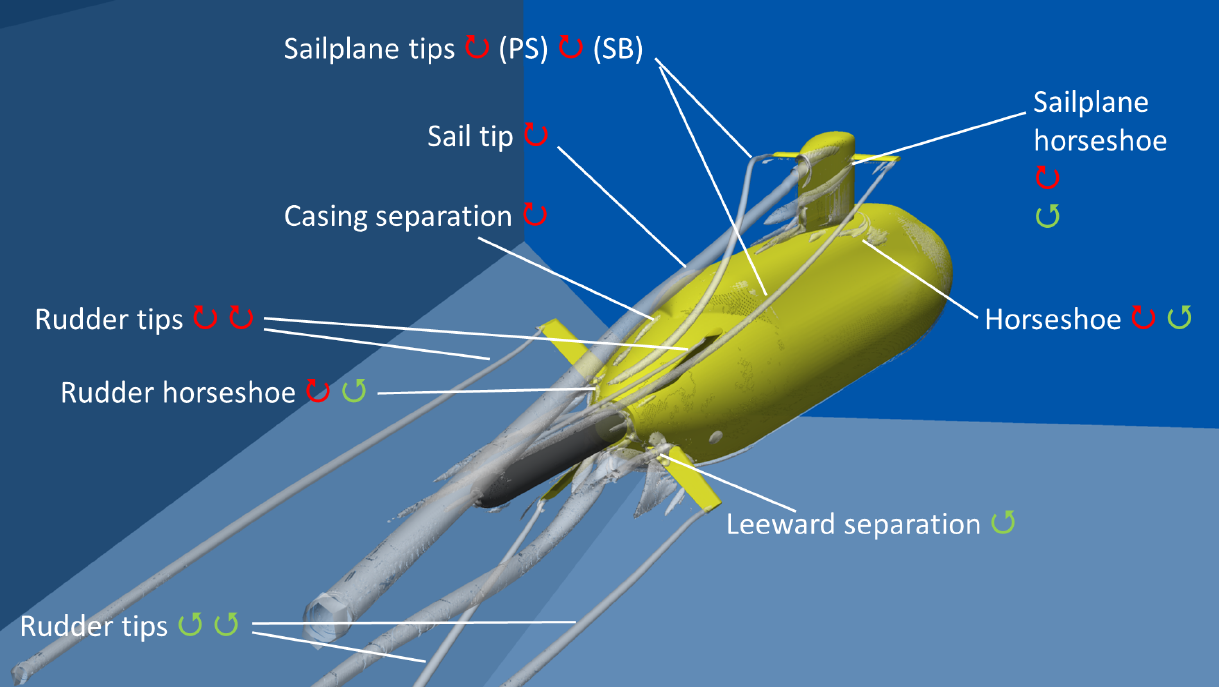
\includegraphics[width=0.45\textwidth]{figs/submarine.png}}}%
    \caption{Examples of non-canonical 3d flows.}%
    \label{fig:examples}%
\end{figure}

\noindent As known from the examples above, different regions of the flow field are characterized by different flow structures, patterns and topology. It is, thus, reasonable to expect that a dedicated model which better reproduces such physics in each region, may improve the global representativity of the simulation. Then, the general definition of the problem can be as follows:
\textcolor{red}{(T1) given a set of GEP models developed for different \textbf{canonical} flows, \textbf{automatically} select the \textbf{best} model in each region of the computational domain for a \textbf{new and unseen}, possibly non-canonical testcase.}

\vspace{10pt}
\noindent There are few keywords to notice in the definition above, which identify several sub-tasks:
\paragraph{Canonical flows.} (ST1) Currently, the available GEP\index{GEP} models have been developed for the following testcases:
\begin{itemize}
    \item 3d square cylinder
    \item 2d airfoil
    \item backfacing step
    \item impinging jet
    \item ...
    \item \textcolor{blue}{experimental or high-fidelity data?}
\end{itemize}
Baseline and GEP\index{GEP}-improved solutions should be available for each testcase. Is it also worth noticing here the importance of the \textbf{identification and selection features and targets} (QoI) for each testcase. These will make up the database which the machine learning algorithm will work on. 

\paragraph{Automatically.} (ST2) We would like to minimize or nullify the human intervention in the model's selection and assignment process. This points to the adoption of a machine or deep learning framework. \textcolor{blue}{Nevertheless, it may be that more traditional methods such as shock/vortex features filters/detectors would be enough?}

\paragraph{Best model.} (ST3) The notion of "best" implies the definition of some metric able to estimate the quality/similarity/correlation between the models available and the flow currently under assessment.

\paragraph{New and unseen.} (ST4) This points to the choice between supervised and unsupervised approach. Given a comparable accuracy between the two methodologies, preference shall be given to unsupervised algorithms in order to get rid of the heavy training phase, as well as the compilation of a database. 

\vspace{10pt}
\noindent Once the aforementioned sub-tasks are fulfilled, the next key question (also from navy guys) is: \textcolor{red}{(T2) how to "blend" different models from different regions?} and consequently how to call and apply each model from the main solver.

\section{The "selector" concept}
In this section, some ideas about how to realize such "model selector" are presented.

\subsection{Data structure}
\textit{The actual implementation of the "selector" appears to be dependent on the type of data structure we are going to process.} Specifically, given the numerical solution of the testcase shall we consider:
\begin{itemize}
    \item 1D data sets (extracted from \index{OpenFOAM@\hypertarget{OpenFOAM.ind}{}OpenFOAM}\href{\#OpenFOAM.ind}{OpenFOAM})
    \item 2D surfaces data (extracted from \index{OpenFOAM@\hypertarget{OpenFOAM.ind}{}OpenFOAM}\href{\#OpenFOAM.ind}{OpenFOAM})
    \item fully 3D data (exported raw solution)
\end{itemize}
Typically, machine and deep learning algorithms are specialized to deal with one preferred data format, thus, \textit{different workflows should be defined depending on the data structure}. 

\textit{Thinking about an "in the loop" approach, it is worth noticing that sets and surfaces are much more "manageable" but are (only?) available at post-processing time while fully 3D data may be available at each solution save time but it requires considerable more time to be processed, if used in toto.}

\subsection{Machine/deep learning algorithm}
Another choice to be made is the selection of the class of algorithms to be employed for the task, namely, supervised or unsupervised (self-supervised, weakly-supervised). 
As stated above, the priority would be given to unsupervised machine learning algorithms in order to avoid the need of large-scale labelled datasets and eventually the associated training process. Consequently, the attention will be "naturally" focused on techniques such as \underline{\textbf{unsupervised} \textbf{clustering}\index{clustering} and \textbf{segmentation}\index{segmentation}}. 
 
\textbf{Cluster\index{clustering} analysis} or clustering\index{clustering} is the task of grouping a set of objects in such a way that objects in the same group (called a cluster\index{clustering}) are more similar (in some sense) to each other than to those in other groups (clusters\index{clustering})\footnote{https://en.wikipedia.org/wiki/Cluster\_analysis}. The objective of clustering is to organise data so that the inner-cluster similarity is maximised while the inter-cluster\index{clustering} similarity is minimised~\cite{kaiser2014cluster}. 
 
\textbf{Semantic segmentation} is the process of classifying each individual pixel of an image into a known ontology~\cite{hamilton2022unsupervised} or equivalently, assigning a class label to every pixel of an image~\cite{van2021unsupervised}. Moreover, if semantic segmentation predicts the labels for every pixel in the input image and each pixel is labelled according to the object class within which it is enclosed, \textbf{instance segmentation} gives different labels for separate instances of objects belonging to the same class. Hence, instance segmentation simultaneously solves the problem of object detection as well as that of semantic segmentation~\cite{hafiz2020survey}. Reasonably, cluster analysis, semantic and instance segmentation shared some common features and they are often used together.

\vspace{10pt}
\noindent \textcolor{blue}{It is worth observing that, the pixel-level classification and segmentation, perhaps, solves the second task (T2) concerning the blending strategy of different models between different regions of the domain. Indeed, having a pixel-by-pixel description would allow to seamlessly assign the model according to the class or segment the pixel belongs to (expensive strategy). More efficiently, an additional field variable may be instantiated in OF, for example, a integer vector with length equal to the number of sub-volumes or models, as well. This will be initialized at t=0, but eventually, it could be read at run time. In this way, it could be re-assigned to a different model.}

\subsubsection{Segmentation of turbulent computational fluid dynamics simulations with
unsupervised ensemble learning~\cite{bussov2021segmentation}}
In~\cite{bussov2021segmentation} an unsupervised clustering ensemble learning technique is used to perform the segmentation of turbulent flow field. From Fig.~\ref{fig:papersconnected}, it is interesting to observe that apparently no other prior or derivative works have dealt with segmentation and clustering of fluid dynamic flow fields and such work appears quite isolated. 

\vspace{10pt}
\noindent According to~\cite{bussov2021segmentation} a workflow with the following features\footnote{\url{https://github.com/mkruuse/segmenting-turbulent-simulations-with-ensemble-learning}} can be devised:
\begin{itemize}
    \item computer vision and machine learning tools are adopted to automate the segmentation of physical structures from 2-dimensional image snapshots 
    \item machine learning clustering algorithms are used for detection and segmentation of visually distinct structures in data (fast enough to be coupled directly into time simulation loop
    \item SCE algorithm is used to average segmentation results from many independent clustering realizations (obtained via SOM algorithm) in order to mitigate the non-deterministic nature of clustering algorithms (influence of initial conditions and different parameters) and obtaining more accurate ROI objects
    \item determine optimal number of meaningful clusters present in the input data
    \item uniquely identify each pixel with the corresponding object cluster
    \item segment clustered pixels into stable contours that can be further analyzed for their geometrical shape, size, and area
    \item each individual clustering realization can be split into different image masks where only the pixels from one specific cluster are "active". Stacking operations of these masks are defined by using the union, intersection, and sum of two masks.
\end{itemize}
%
\begin{figure}[H]%
    \centering
    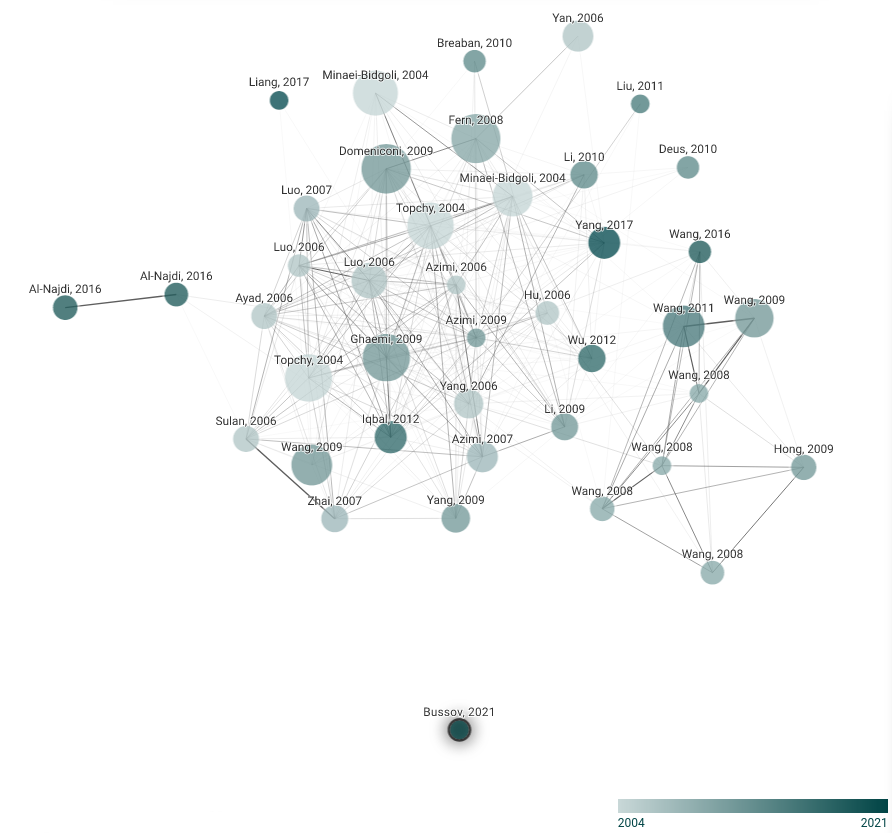
\includegraphics[width=0.7\textwidth]{figs/papersconnected.png}
    \caption{Visual graph of connected papers for~\cite{bussov2021segmentation}.}
    \label{fig:papersconnected}%
\end{figure}
%
Some other works~\cite{van2021unsupervised,hamilton2022unsupervised,ji2019invariant,caron2018deep} proposed even more effective and efficient segmentation and clustering\index{clustering} techniques, nevertheless not targeted for fluid dynamic applications. In~\cite{kaiser2014cluster}, a cluster-based reduced-order modelling of a mixing layer was considered. An increasing number of publications adopting segmentation and clustering techniques for medical imagine application, can be found in literature, such as~\cite{colebank2019influence}.

\subsubsection{Deep learning for 3D point clouds: a survey~\cite{guo2020deep}}
If we accept to abandon or at least partially deviate from the choice of using strictly only unsupervised algorithms, we number of publications increases significantly. In particular, if we retain the idea of working with 3D data (no extracted sets or surfaces from OF) we need consider algorithms able to handle clouds of points~\ref{fig:taxo}. In this regards, very informative is the recent review~\cite{guo2020deep} whose visual graph of connected papers is reported in Fig.~\ref{fig:guo}. The impact of such publication is apparent from the size of the corresponding circle as well as the rich network of citations.
%
\begin{figure}[H]%
    \centering
    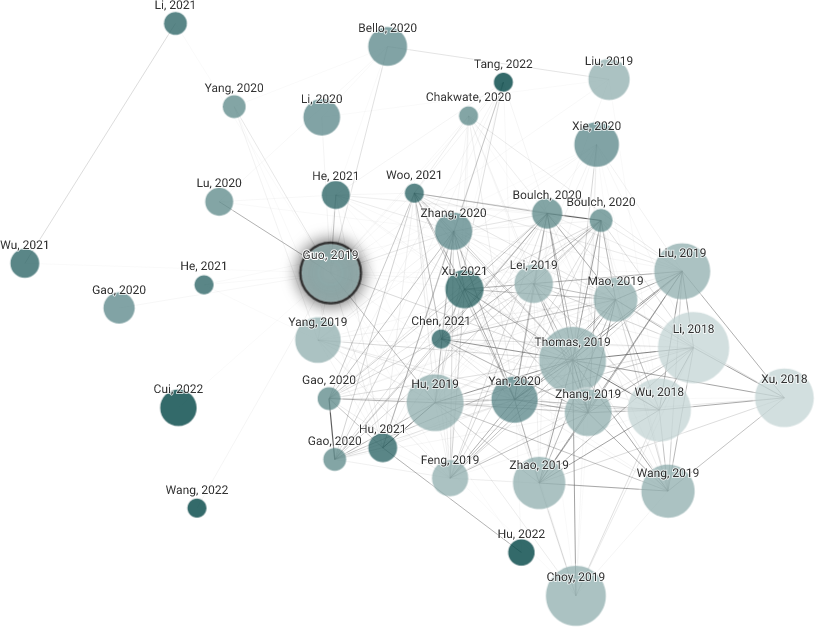
\includegraphics[width=0.7\textwidth]{figs/guo.png}
    \caption{Visual graph of connected papers for~\cite{guo2020deep}.}
    \label{fig:guo}%
\end{figure}
%
\noindent From~\cite{guo2020deep}, many different methods and architectures can be adopted for our task, in terms of classification, clustering, detection and segmentation. In particular, as suggested in~\cite{sun2021automated}, the following automated simulation framework data-driven turbulence modeling workflow can be developed:
\begin{enumerate}
    \item Data acquisition and preprocessing (OF solutions).
    \item Point cloud segmentation based on deep learning: perform a semantic segmentation of the point clouds, which divides the point clouds according to their physical significance. A filter may be applied at this stage (Gabor, Sobel, ...). Subsequently, the point clouds are segmented using deep learning, (possibly reducing the work of feature engineering and enhancing the capture of local features). The method may combine 2D network, (DeepLabv3)\footnote{https://paperswithcode.com/method/deeplabv3}, and 3D network, (PointNet++)\footnote{https://paperswithcode.com/paper/pointnet-deep-hierarchical-feature-learning}. The point clouds are first rasterized into 2D images as the input of DeepLabv3, which subsequently predicts the probability vectors of pixel-by-pixel classification and maps them back to the points. Finally, the point clouds are sparsified and input into PointNet++ to obtain point-by-point classification results.
    \item Geometric 3D reconstruction: after obtaining the respective point clouds, it is necessary to establish clean and low-complexity models of the target area, which are suitable for CFD simulation.
    \item CFD modeling and simulation: the 3D models in STL format generated for each sub-region are directly imported into OF. Grids are generated using its automatic grid generation function. To perform a CFD simulation, the sub-regions are assigned different GEP model (if necessary w.r.t. the baseline) by implementing an automated script based on the labels identified by the clustering phase.
\end{enumerate}

\begin{sidewaysfigure}
    \centering
    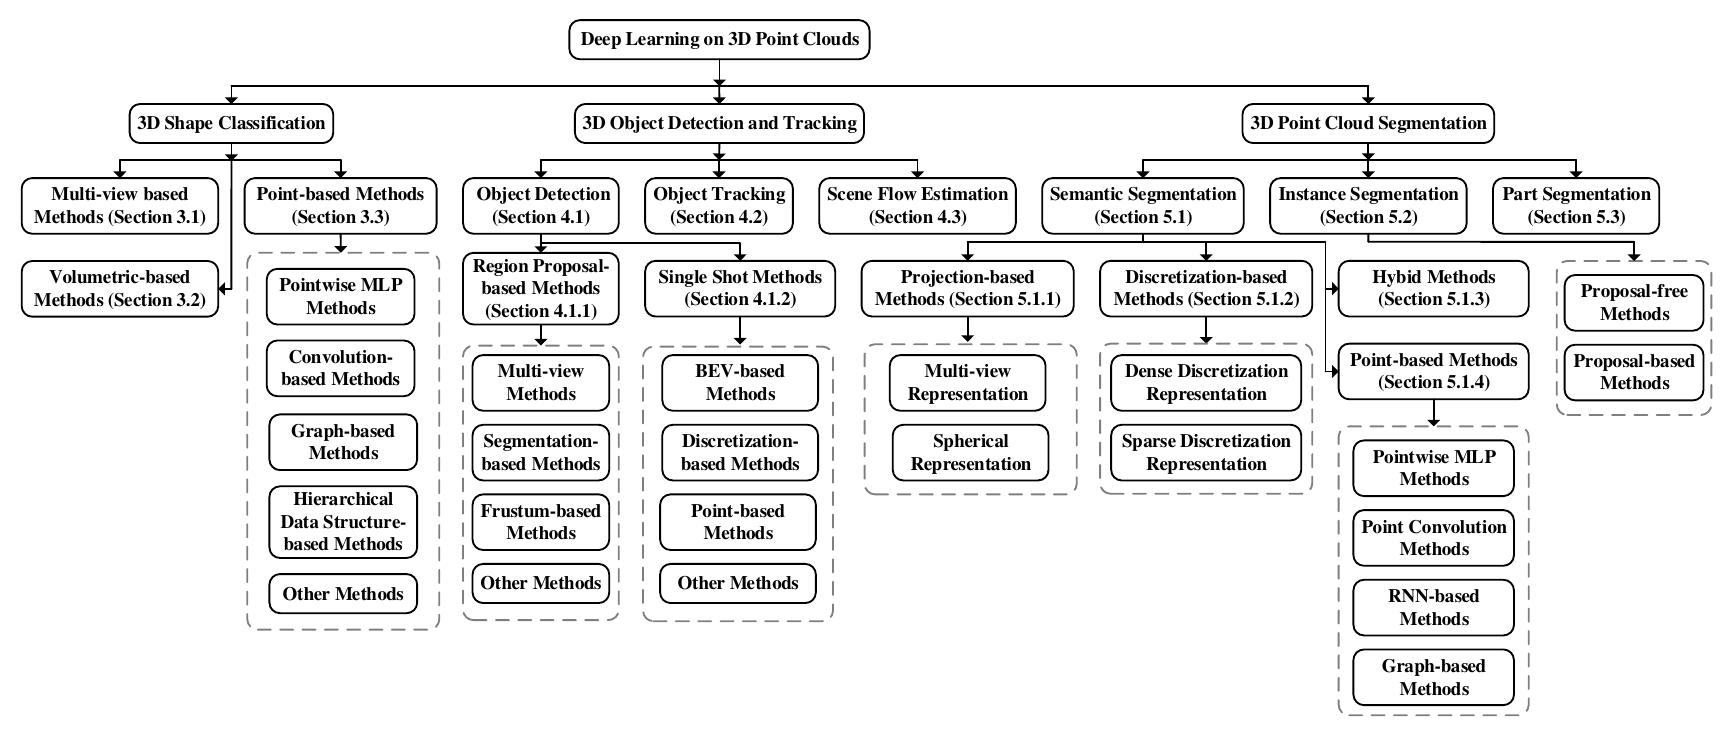
\includegraphics[width=1.0\textwidth]{figs/taxonomy.png}
    \caption{A taxonomy of deep learning methods for 3D point clouds~\cite{guo2020deep}.}
    \label{fig:taxo}%
\end{sidewaysfigure}

\subsubsection{Unsupervised Semantic Segmentation by Distilling Feature Correspondences}
\url{https://github.com/mhamilton723/STEGO}\\
\url{https://github.com/facebookresearch/dino}\\
\url{https://github.com/facebookresearch/DeeperCluster}\\
\url{https://github.com/facebookresearch/swav}\\

\begin{figure}
    \centering
    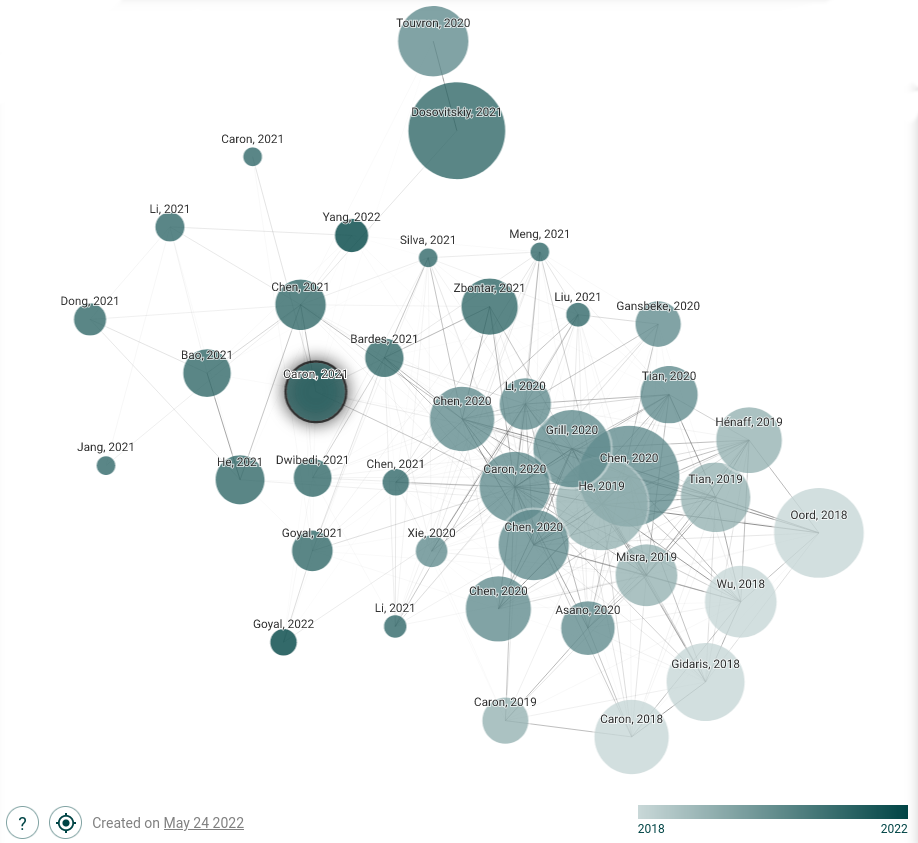
\includegraphics[width=0.75\textwidth]{figs/dino.png}
    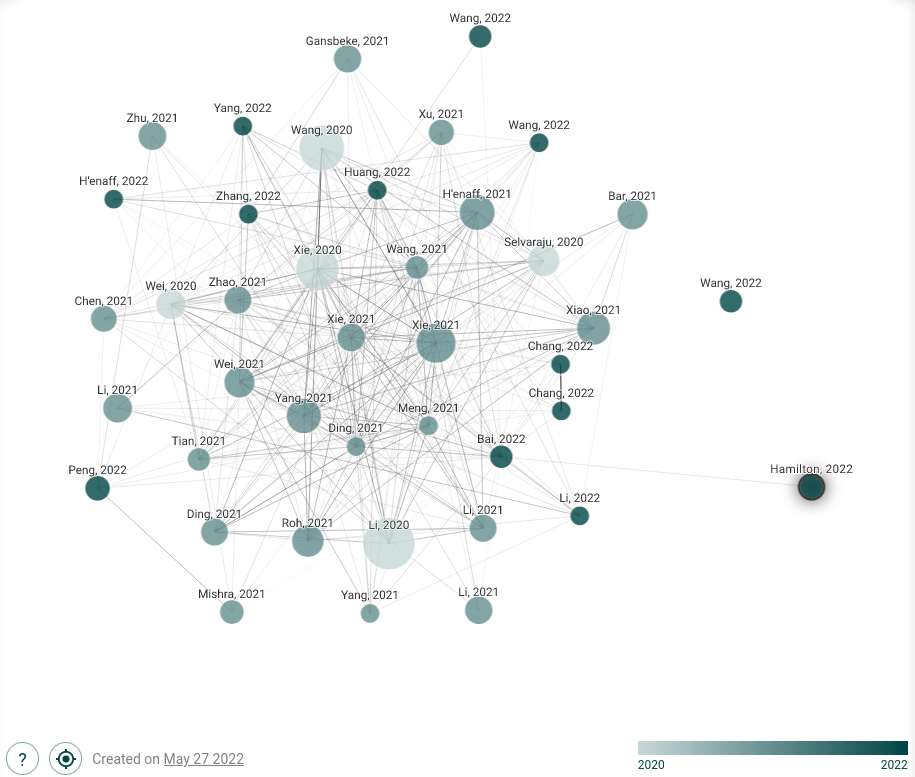
\includegraphics[width=0.75\textwidth]{figs/stego.png}
    \caption{Visual graph of connected papers for DINO~\cite{caron2021emerging} and STEGO~\cite{hamilton2022unsupervised}.}
    \label{fig:DINO_STEGO}%
\end{figure}

\subsection{Clustering}
%https://www.r-bloggers.com/2019/01/10-tips-for-choosing-the-optimal-number-of-clusters/
In this section, the progress about clustering analysis for data-driven turbulence modeling will be reported. A general overview on this class of algorithms can be found in~\cite{bouveyron2019model,giordani2020introduction,skiadas2019data}.

It should be soon realised that the clustering\index{clustering} problem which we are tackling is far more challenging than traditional examples. Indeed, if for example consider the typical Iris database~\ref{tab:iris}, we have only four features and three species to be clustered, while in our case we may possibly have more targets corresponding to each point of the computational domain to be clustered and each point has many more features which it may depend upon, corresponding to the QoI from the flow field solution, as exemplified in~\ref{tab:reality}. Thus, at least in the present formulation, the problem will certainly benefit from a \textbf{dimensionality reduction} as well as a \textbf{feature selection} pre-processing step.
%
\begin{table}[H]
\begin{centering}
\begin{tabular}{ccccc}
Sepal.length & Sepal.width & Petal.length & Petal.width & Species\tabularnewline
\hline
\hline
. & . & . & . & setosa\tabularnewline
\hline
. & . & . & . & virginica\tabularnewline
\hline
. & . & . & . & versicolor\tabularnewline
\hline
\end{tabular}
\par\end{centering}
\caption{\label{tab:iris}Exemplification of Iris database}
\end{table}
%
\begin{table}[H]
\begin{centering}
\begin{tabular}{cccccccccc}
$a_{ij}\left[6\right]$ & $R\left[6\right]$ & \textbf{$u\left[3\right]$} & $I_{i}\left[5\right]$ & $T_{i}\left[10\right]$ & k & $\omega$ & $\nu_{t}$ & ... & Points\tabularnewline
\hline
\hline
. & . & . & . & . & . & . & . & . & 1\tabularnewline
\hline
. & . & . & . & . & . & . & . & . & 2\tabularnewline
\hline
. & . & . & . & . & . & . & . & . & .\tabularnewline
\hline
. & . & . & . & . & . & . & . & . & n\tabularnewline
\hline
\end{tabular}
\par\end{centering}
\caption{\label{tab:reality}Example of a realistic database}
\end{table}

%\vspace{10pt}
%Some interesting projects are reported below:\\
%\url{https://github.com/xu-ji/IIC} \\
%\url{https://github.com/wvangansbeke/Unsupervised-Semantic-Segmentation} \\
%\url{https://github.com/mhamilton723/STEGO} \\
%\url{https://github.com/hbilen/wsl-eccv20.github.io} \\
%\url{https://github.com/facebookresearch/moco/fork} \\
%\url{https://github.com/facebookresearch/swav} \\
%\url{https://github.com/facebookresearch/deepcluster}

\subsection{Unsupervised detection, segmentation and clustering}
As preferred choice, an unsupervised approach will be pursued. In particular, a three-dimensional unsupervised clustering method will be sought. In this regards, the review paper~\cite{xiao2022unsupervised} is of particular interest\footnote{\url{https://github.com/xiaoaoran/3d_url_survey}}.

\subsection{Dimensionality reduction}
One immediate issue which arises from the high-dimensionality of the database is to visualize or more precisely to find an appropriate mapping to a two- or three-dimensional space which preserves pairwise similarities as well as possible. 

Among the wide range of choice\footnote{https://scikit-learn.org/stable/modules/decomposition.html\#decompositions},\footnote{https://scikit-learn.org/stable/modules/manifold.html}, an interesting option seems to be the t-SNE algorithm~\cite{van2008visualizing} due to its properties. The main idea behind t-SNE\index{t-SNE} is to map a high-dimensional space $X$ to a low-dimensional space $Y$ where the distribution of pairwise similarities is preserved as much as possible. Similarity between data points $x_i$, $x_j$ $\in$ $X$ is defined as the probability that $x_i$ would pick $x_j$ as its neighbor. A similar probability distribution is found in $Y$ by minimizing the Kullback-Leibler divergence between the two distributions
using gradient descent. 

% https://stats.stackexchange.com/questions/263539/clustering-on-the-output-of-t-sne
Nevertheless, t-SNE\index{t-SNE} does not preserve distances nor density. It only to some extent preserves nearest-neighbors. The difference is subtle, but affects any density- or distance-based algorithms.
While clustering after t-SNE\index{t-SNE} will sometimes (often?) work, it may be difficult to explain the clusters, as we may just see 'shapes in clouds' not necessarily clear whether real or artifacts. Therefore, applying any clustering algorithms after t-SNE\index{t-SNE} may not be a good starting point since the initial data may be heavily distorted, and neither distances nor density are preserved well.

At present, a viable option seems to be LargeVis~\cite{tang2016visualizing} which implements an optimized version of t-SNE\index{t-SNE} and reports good scalability properties.

\section{Workflow}
At the moment the preferred framework to compare clustering algorithms is R~\cite{team2013r} as well as the implementation of scikit-learn~\cite{pedregosa2011scikit}. The two environments are compatible with each other and conversion into one or another is easily done.

\vspace{10pt}
\noindent The adopted workflow is the following:
\begin{itemize}
    \item Consider the solution or the surface data extracted at the last time. Extracted surfaces are somehow better because they include the position coordinates. Moreover, the exporting of the solution as a spreadsheet can be quite long for refined meshes and a large number of variables.
    \item Convert it to a \texttt{csv} file which will constitute the database for the further clustering. This step is performed by running a script which saves all the QoI from different planes of the computational domain in corresponding files.
    \item An itermediate pre-processing step may be included in order to concatenate/split different solution fields (input features) into one/several files. At this stage, feature selection or model reduction may be applied.
    \item Run clustering algorithm for each testcase (canonical and current). {As result from the clustering and/or segmentation analysis, we will have a certain number of clusters containing a three-dimensional portion of the domain whose points are labelled according to their physical meaning.} 
    \item Once the list of points for each region and their physical labels are known for the target simulation, they can be compared with the canonicals' ones to compute a "similarity metrics". The best performing metric will identify which model should be used for each sub-region.
    \item The list of points for each sub-region, their physical labels and the metric can be imported into the solver and used to select and assign the model.
\end{itemize}

\vspace{10pt}
\underline{Among unknown ones, few possible issues and observations ...}
\begin{itemize}
\item Three-dimensional nature of the domain, while clustering analysis is typically applied on two-dimensional planes.
\item Complex flow topology, as shown in Fig.~\ref{fig:streamlines}, which makes difficult to obtain a clean clustering or closed surfaces to be directly imported in OF (some filtering may be necessary).
\item Size of the simulations make post-processing and/or conversions quite resources consuming (this would point to minimal end-to-end interference).
\item Baseline or the GEP-augmented solution should be used? In any case, a fixed set of variables should be selected for the machine learning "filtering" stage (this points to a feature importance analysis for each testcase).
\item \textcolor{green}{The final output of the clustering/segmentation processing stage could be an STL surface which encapsulates a sub-volume region of the full domain. The number of these sub-volumes should correspond to the number of available models to be selected. Thus, an additional field variable may be instantiated in OF, for example, a integer vector with length equal to the number of sub-volumes or models, as well. This will be initialized at t=0, but eventually, it could be read at run time. In this way, it could be re-assigned to a different model.}
\end{itemize}

\begin{figure}[H]%
    \centering
    \subfloat[\centering velocity gradient magnitude]{{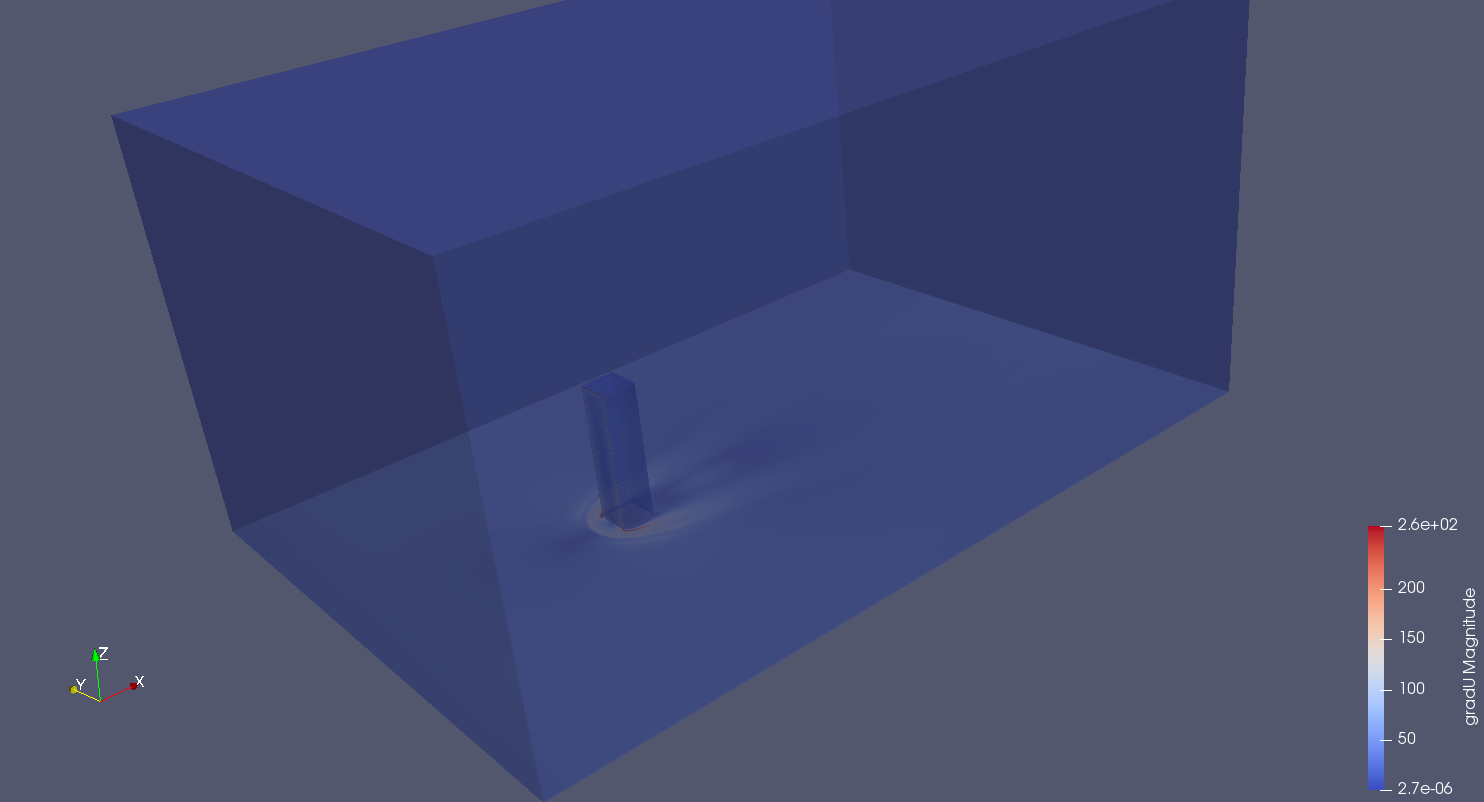
\includegraphics[width=0.45\textwidth]{figs/sqcyl/gradU.png}}}%
    \qquad
    \subfloat[\centering velocity magnitude]{{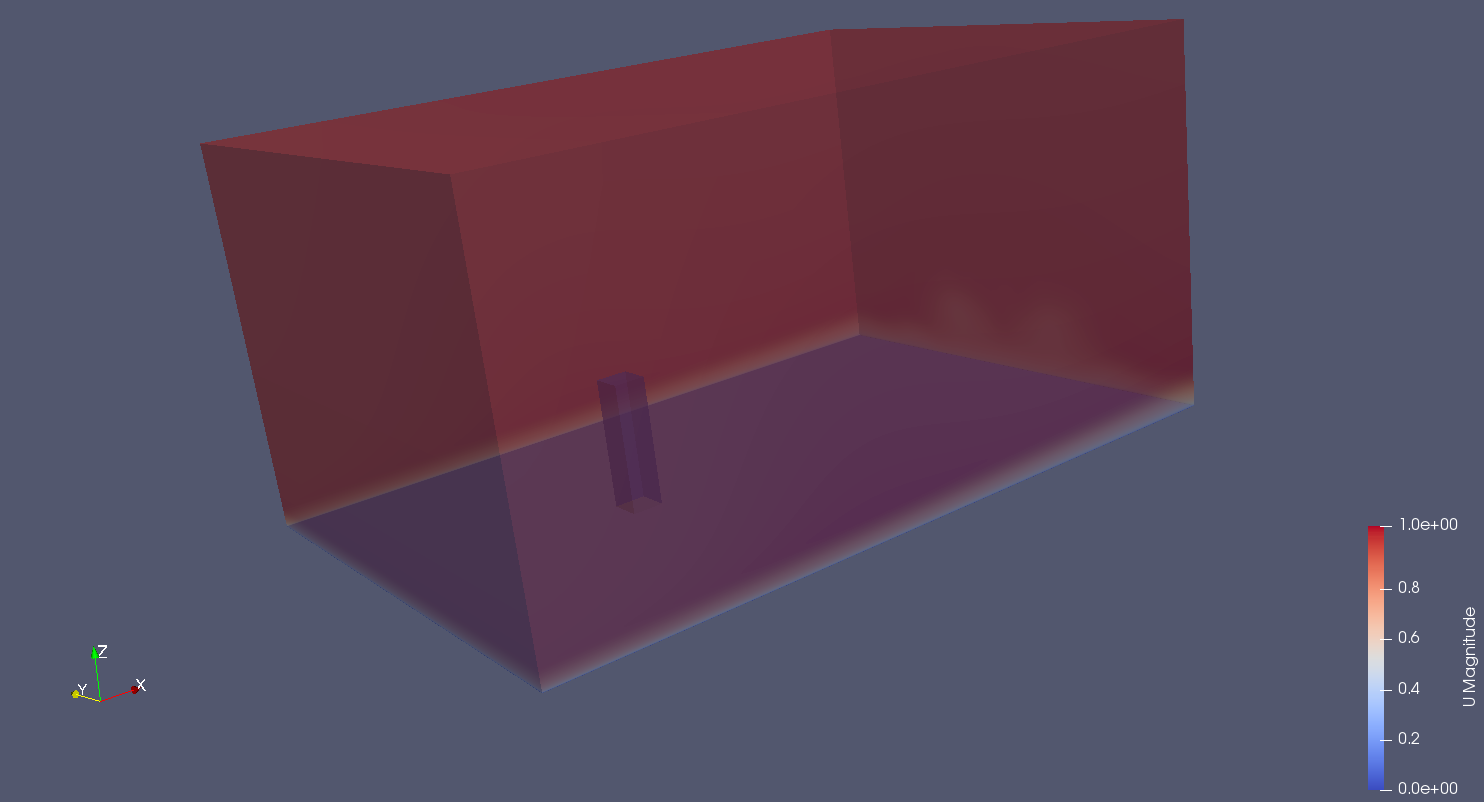
\includegraphics[width=0.45\textwidth]{figs/sqcyl/U.png}}}%
    \caption{}%
    \subfloat[\centering $a_{ij}^x$ magnitude]{{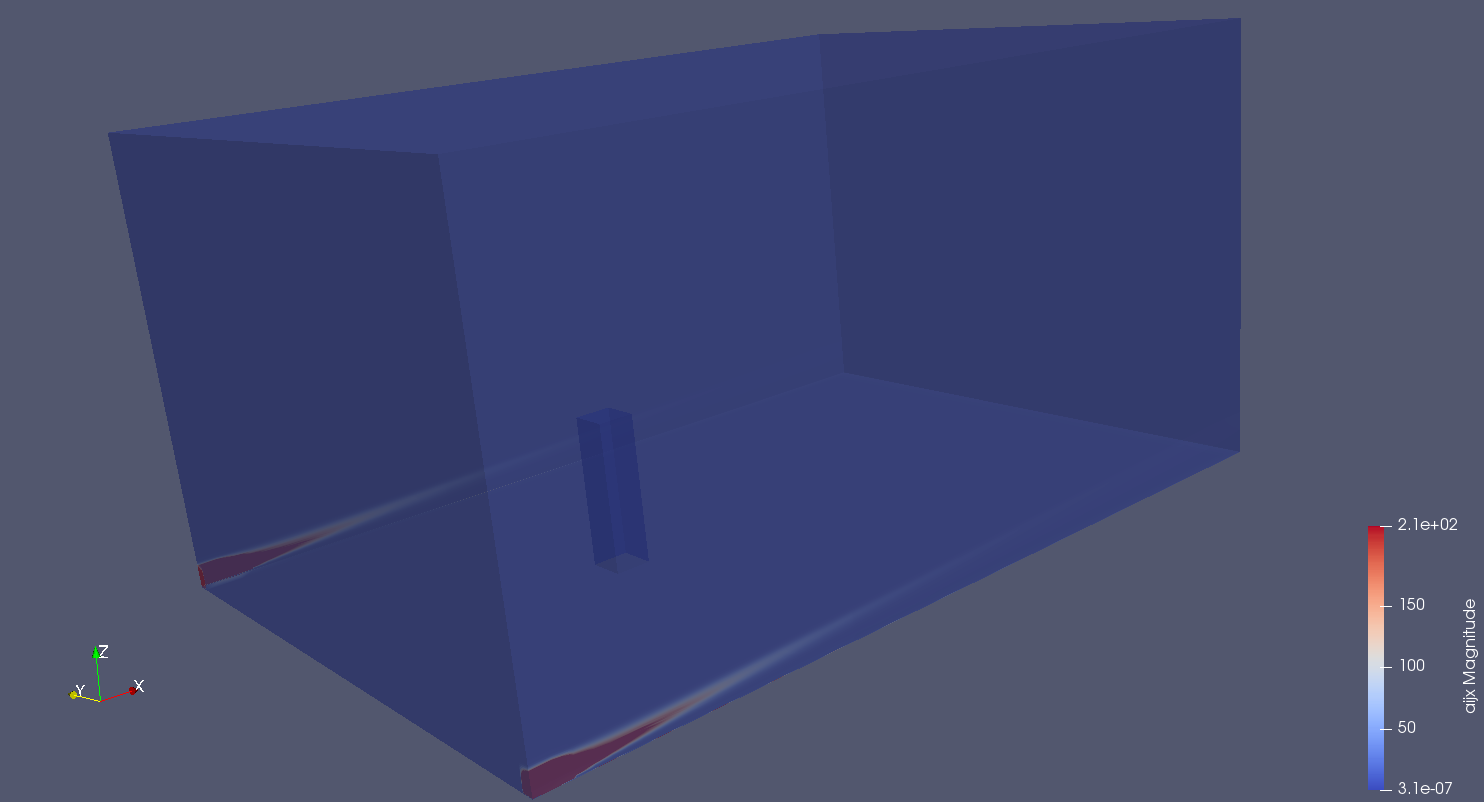
\includegraphics[width=0.45\textwidth]{figs/sqcyl/aij_magn.png}}}%
    \qquad
    \subfloat[\centering $a_{ij}^{yy}$]{{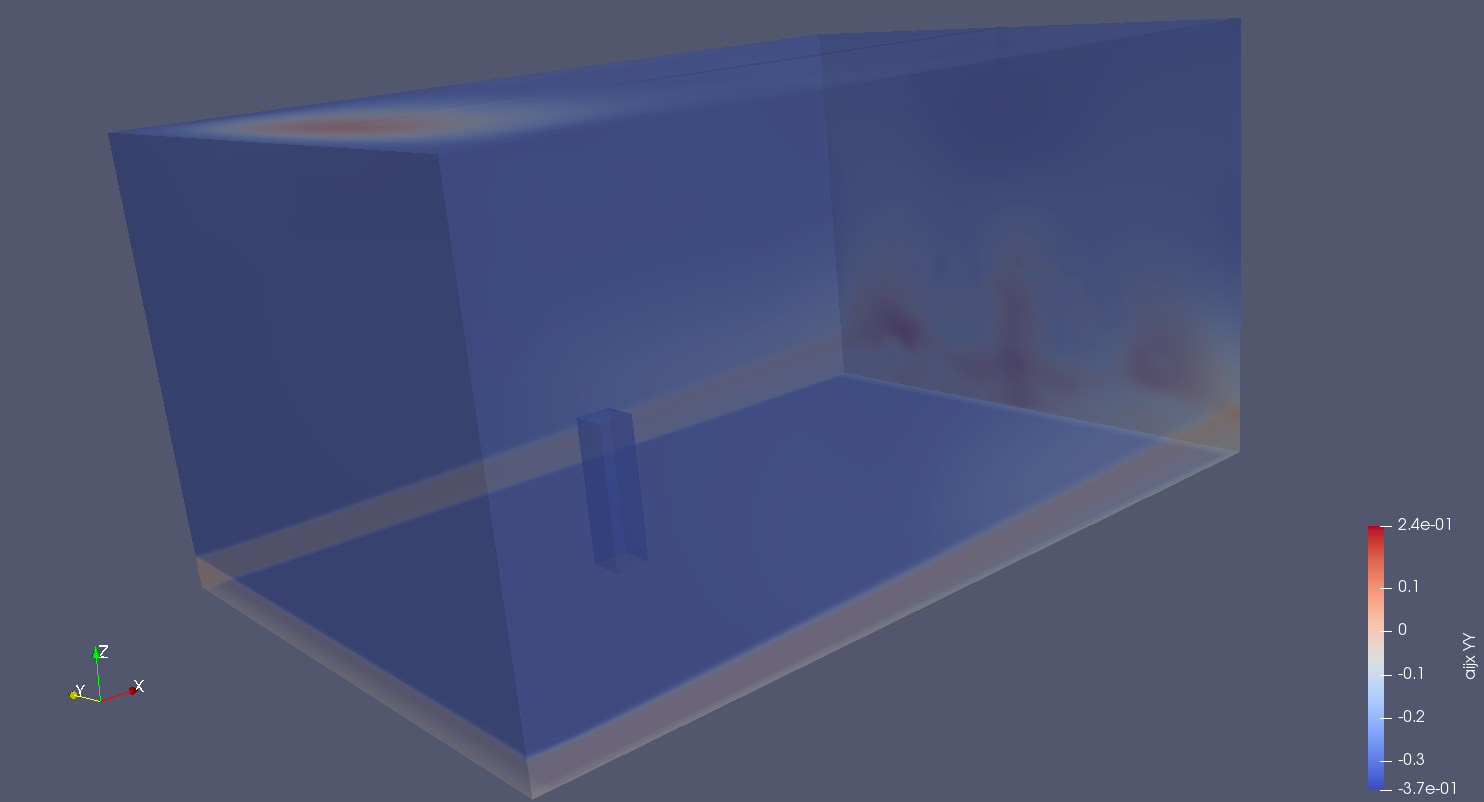
\includegraphics[width=0.45\textwidth]{figs/sqcyl/aij_yy.png}}}%
    \caption{}%
    \subfloat[\centering $k$]{{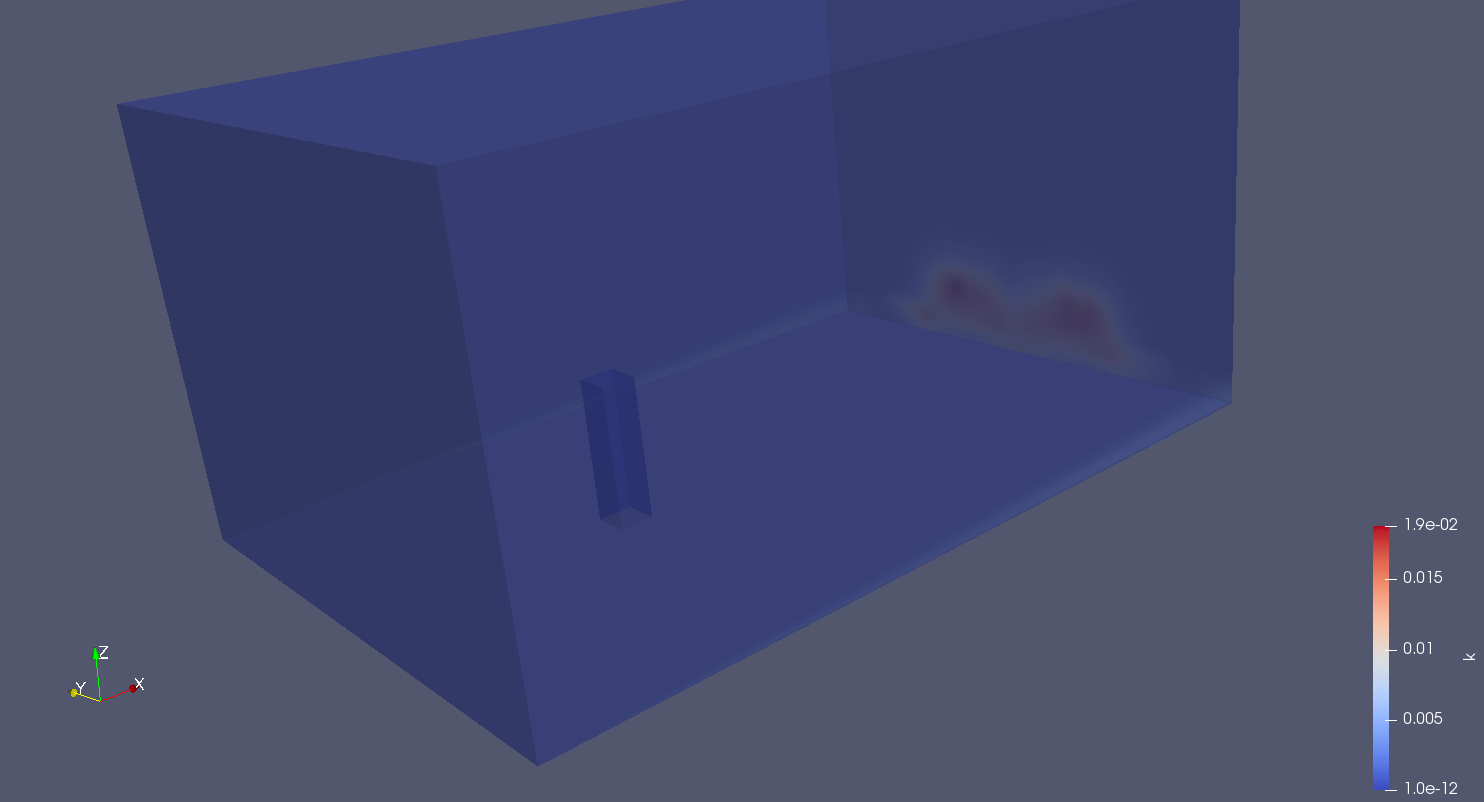
\includegraphics[width=0.45\textwidth]{figs/sqcyl/k.png}}}%
    \qquad
    \subfloat[\centering $\omega$]{{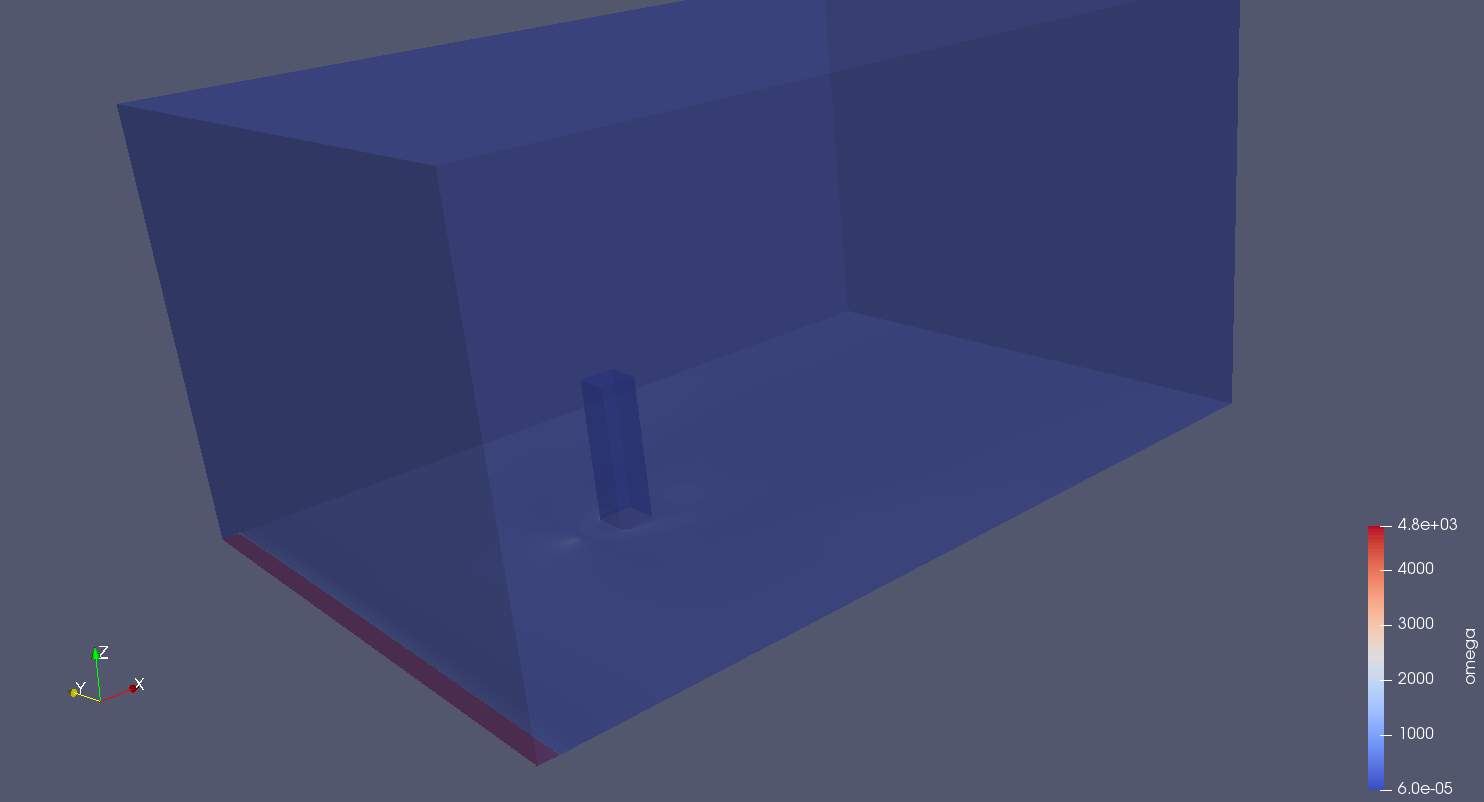
\includegraphics[width=0.45\textwidth]{figs/sqcyl/omega.png}}}%
    \caption{}%
    \subfloat[\centering $S_{ij}$ magnitude]{{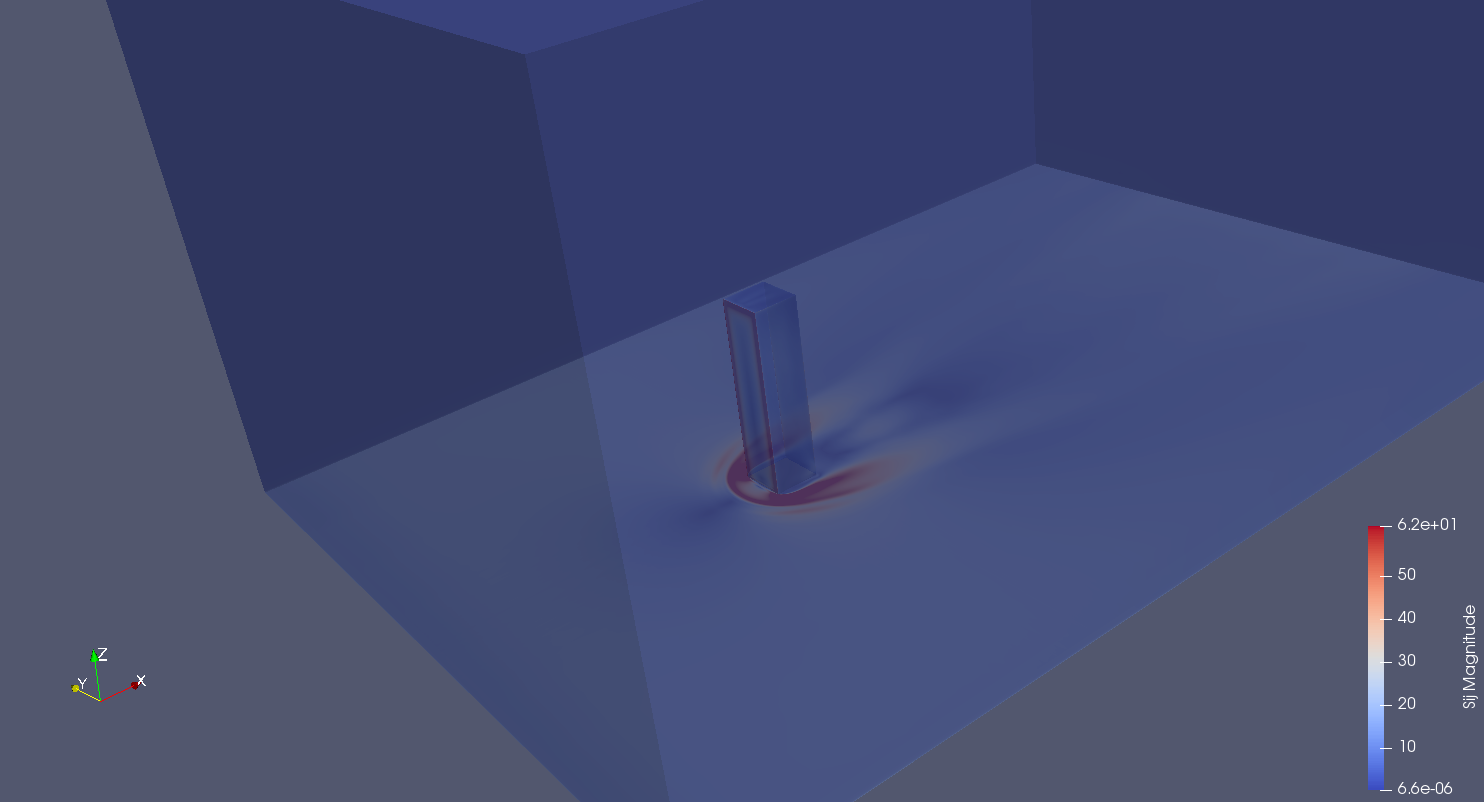
\includegraphics[width=0.45\textwidth]{figs/sqcyl/Sij.png}}}%
    \qquad
    \subfloat[\centering $\Omega_{ij}$ magnitude]{{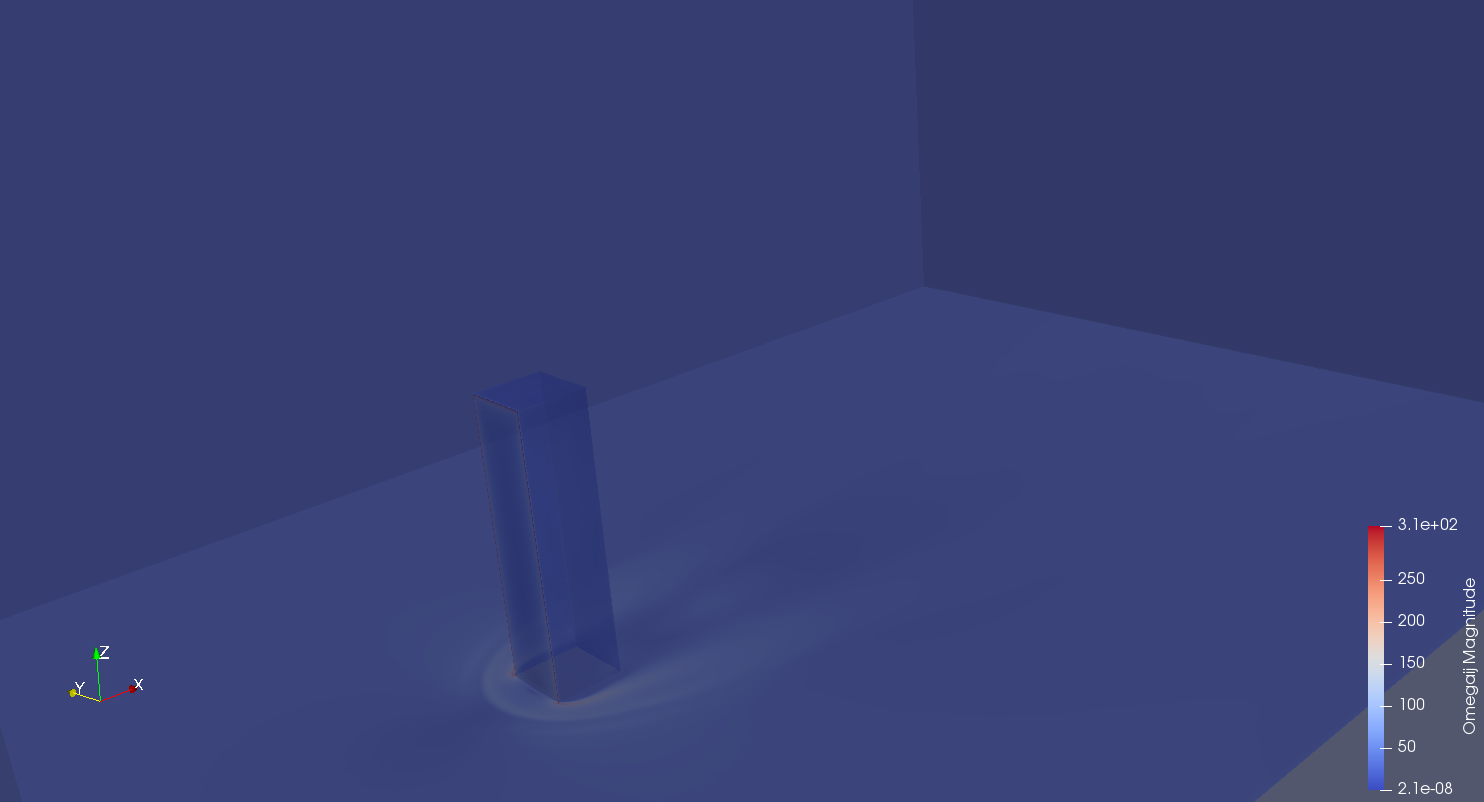
\includegraphics[width=0.45\textwidth]{figs/sqcyl/Omegaij.png}}}%
    \caption{}%
    \label{fig:sqcyl}%
\end{figure}

\begin{figure}[H]%
    \centering
    \subfloat[\centering $b_{ij}$ magnitude]{{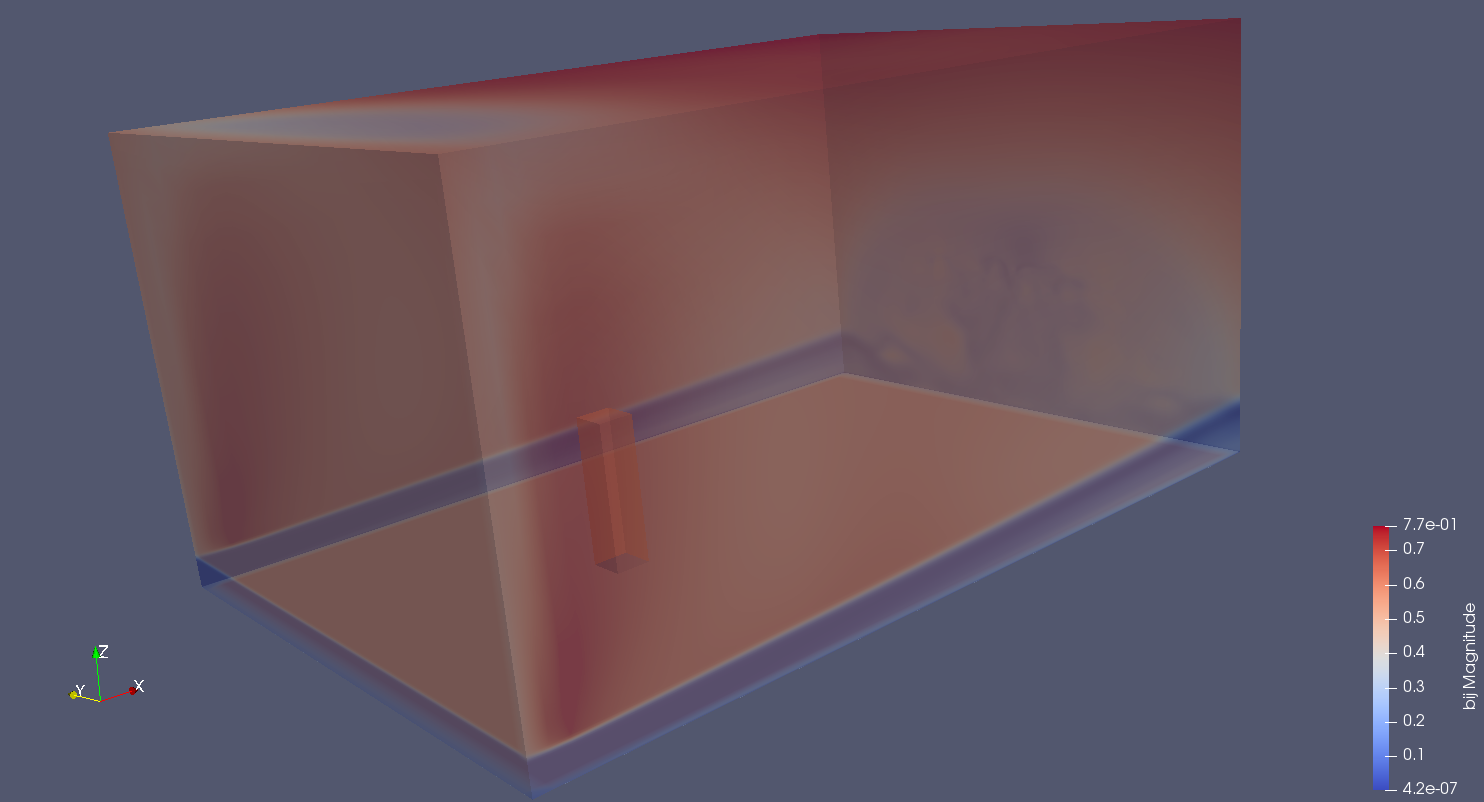
\includegraphics[width=0.45\textwidth]{figs/sqcyl/bij_magn.png}}}%
    \qquad
    \subfloat[\centering $b_{ij}^{xx}$]{{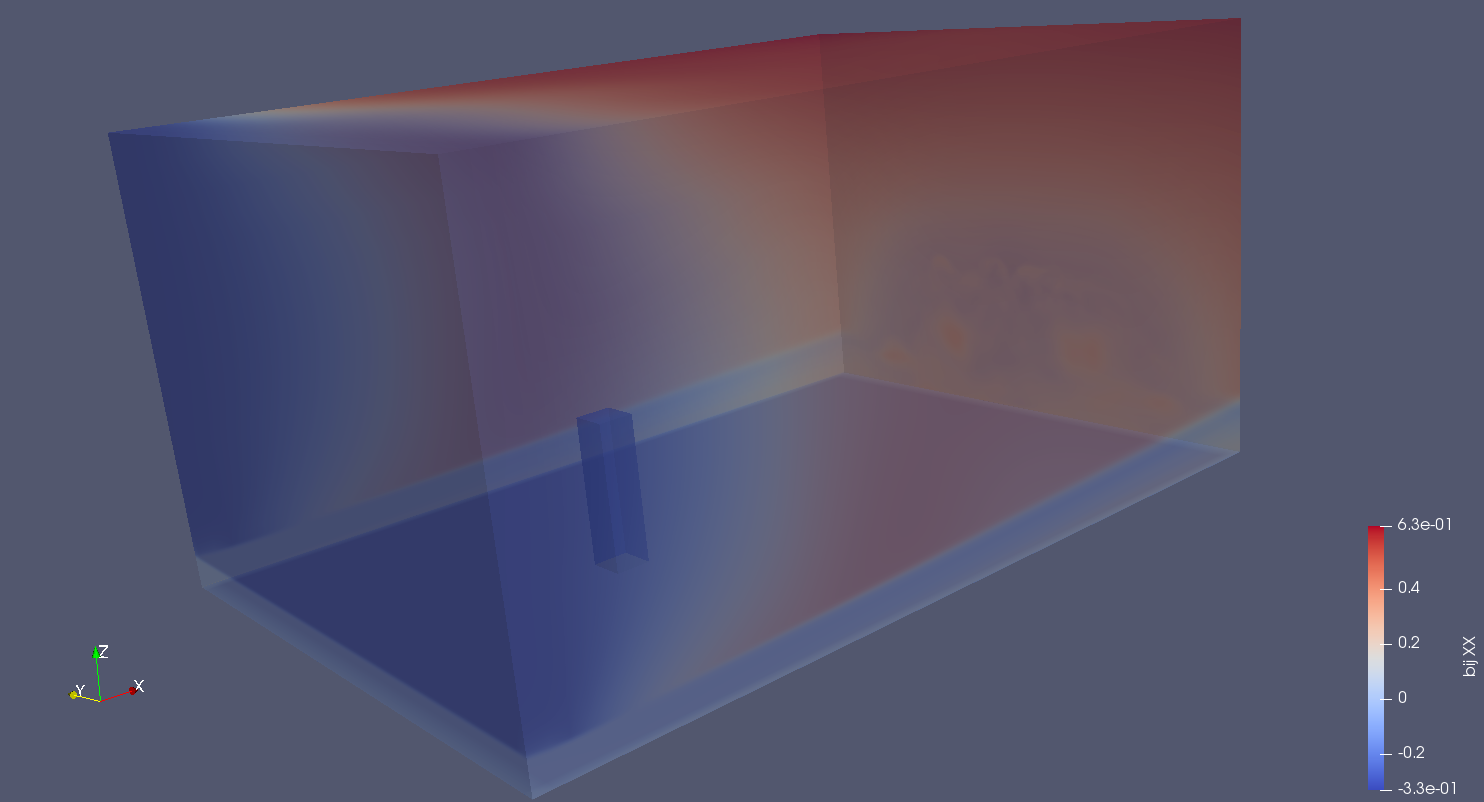
\includegraphics[width=0.45\textwidth]{figs/sqcyl/bij_xx.png}}}%
    \caption{}%
    \subfloat[\centering $b_{ij}^{xy}$]{{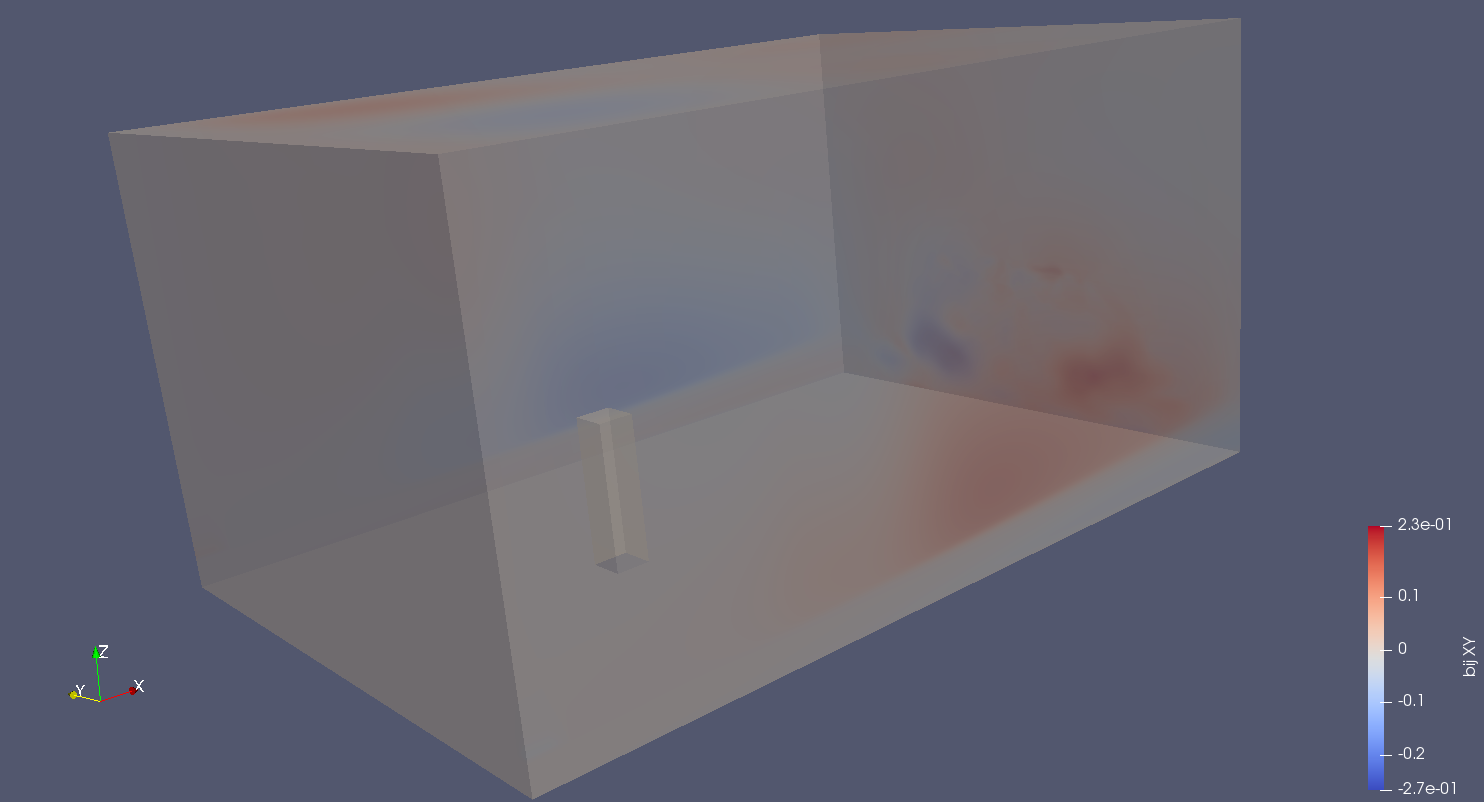
\includegraphics[width=0.45\textwidth]{figs/sqcyl/bij_xy.png}}}%
    \qquad
    \subfloat[\centering $b_{ij}^{xz}$]{{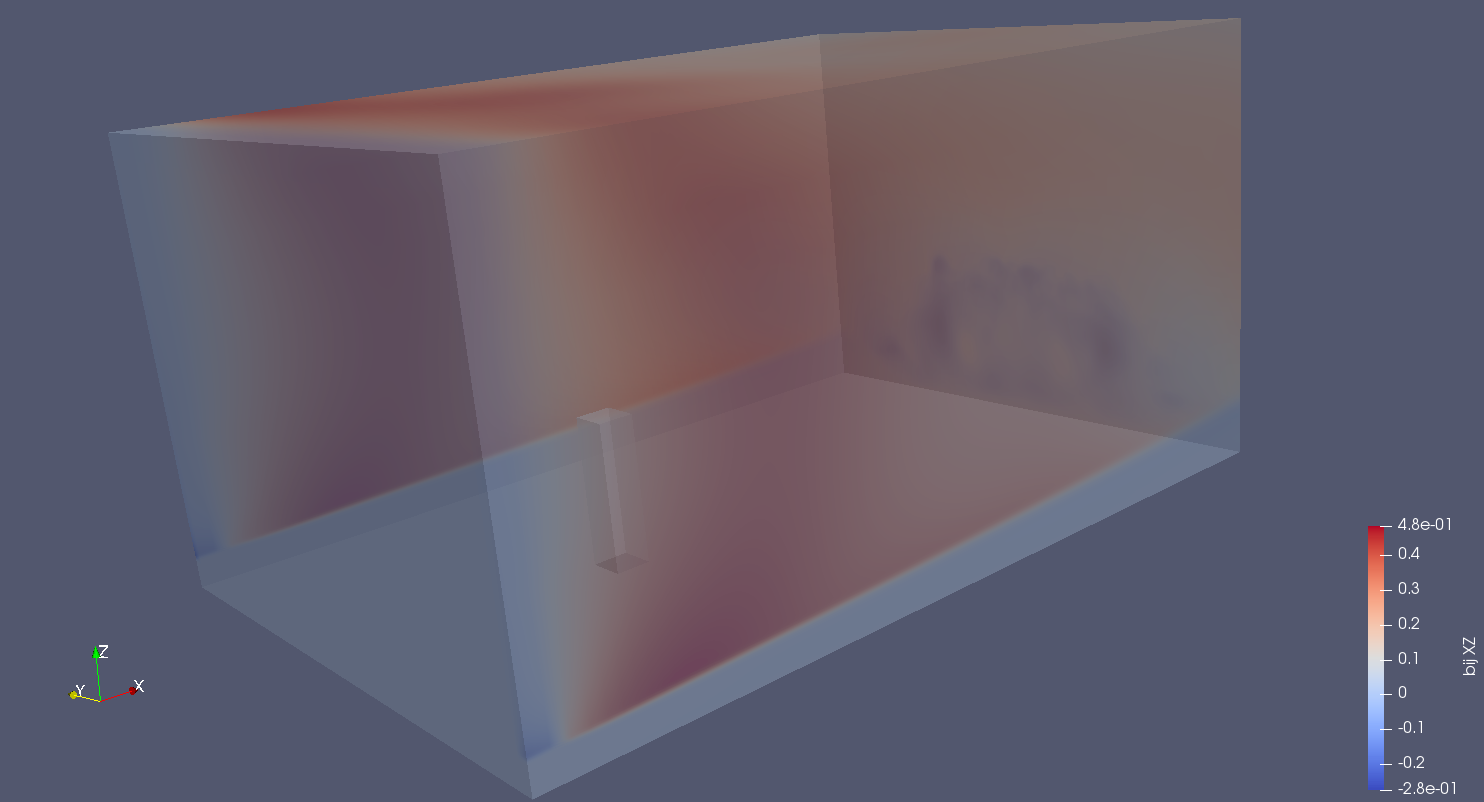
\includegraphics[width=0.45\textwidth]{figs/sqcyl/bij_xz.png}}}%
    \caption{}%
    \subfloat[\centering $b_{ij}^{yy}$]{{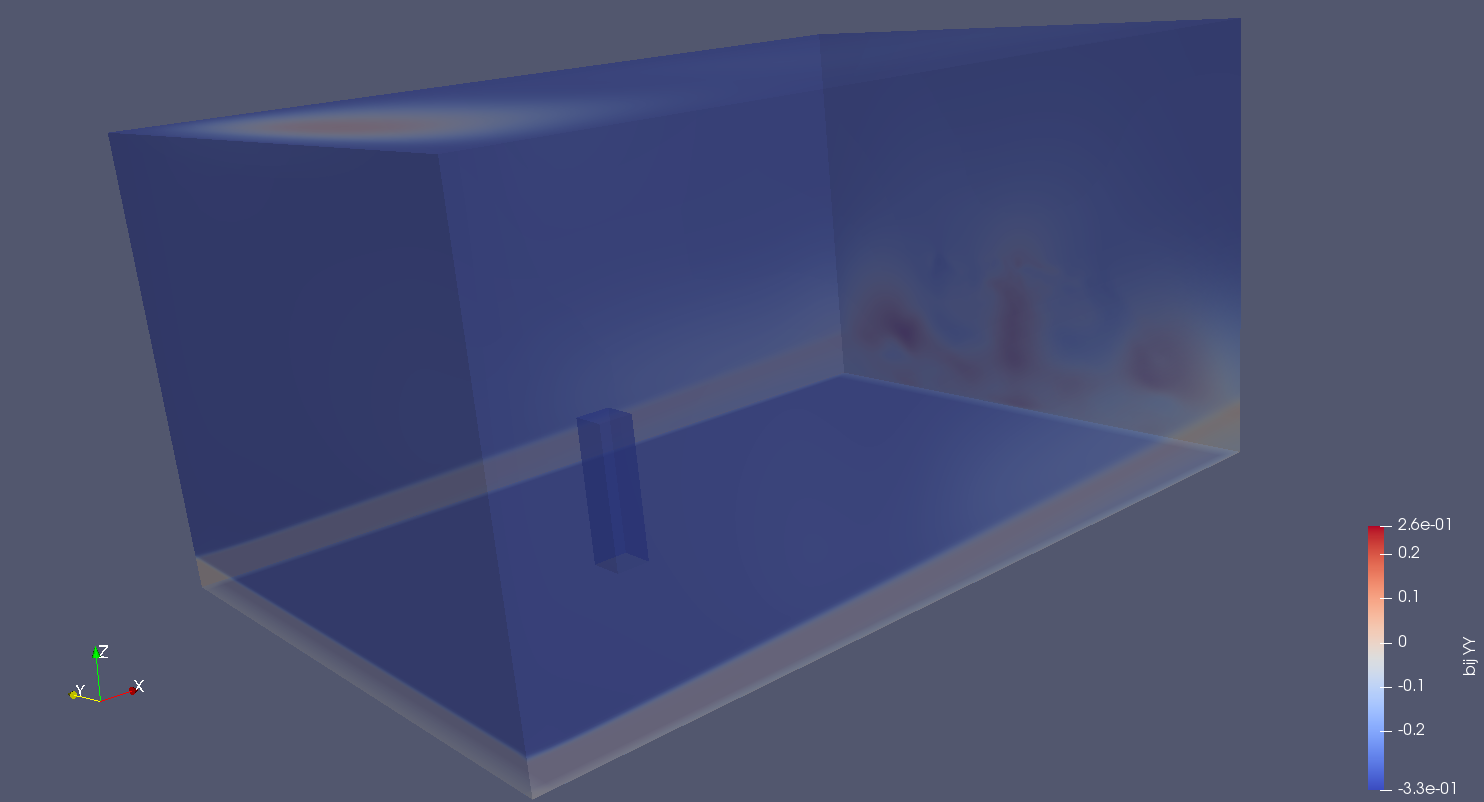
\includegraphics[width=0.45\textwidth]{figs/sqcyl/bij_yy.png}}}%
    \qquad
    \subfloat[\centering $b_{ij}^{yz}$]{{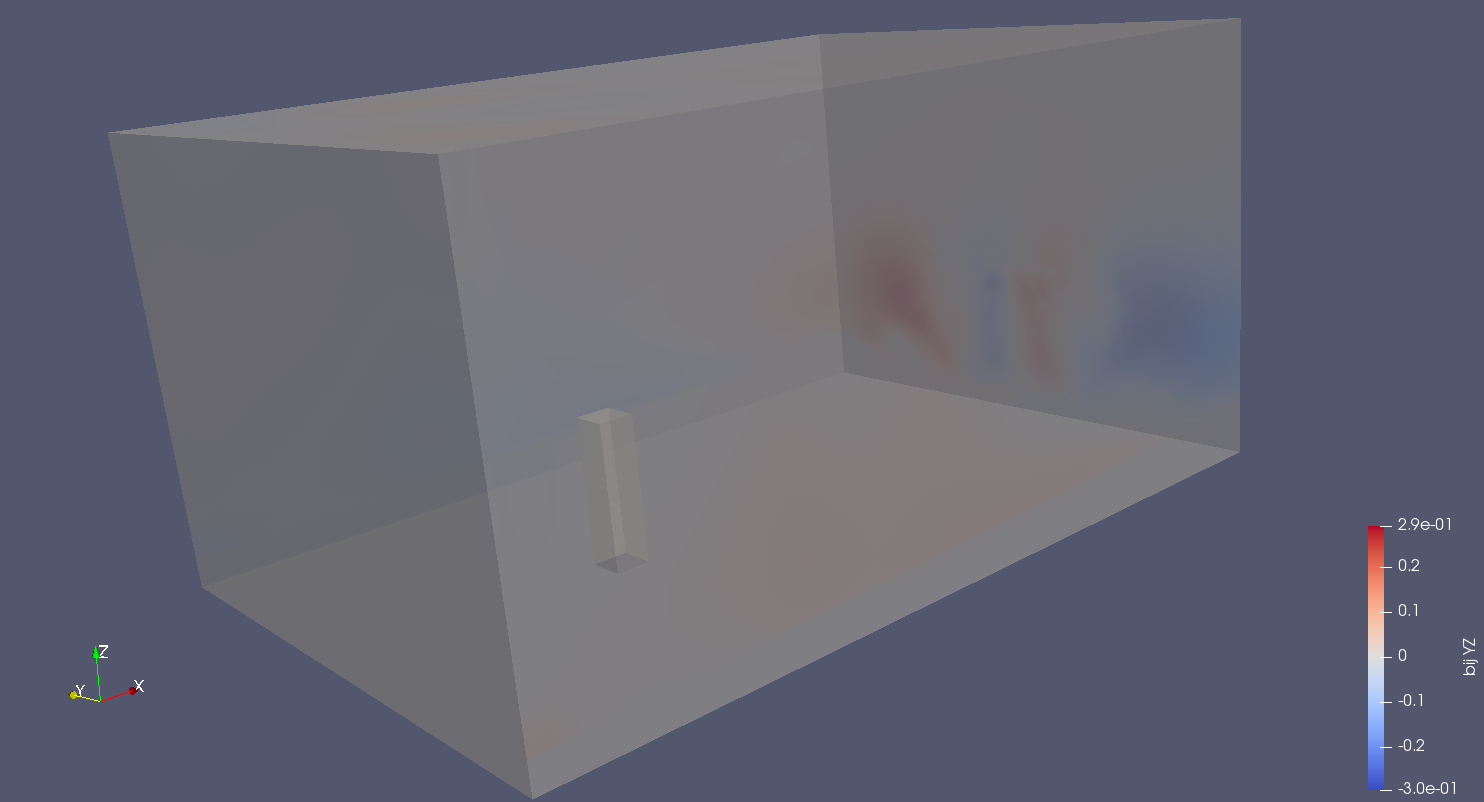
\includegraphics[width=0.45\textwidth]{figs/sqcyl/bij_yz.png}}}%
    \caption{}%
    \subfloat[\centering $b_{ij}^{zz}$]{{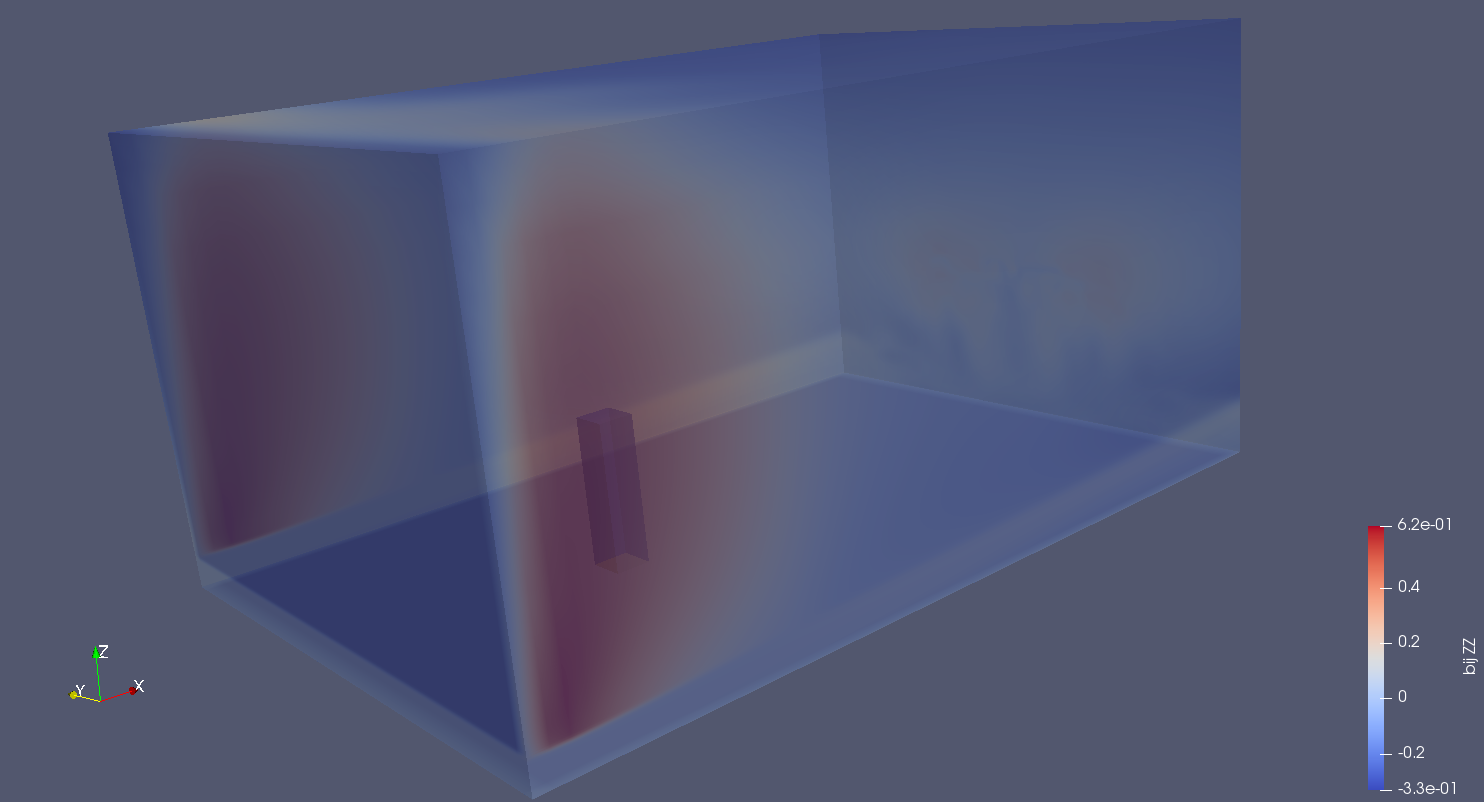
\includegraphics[width=0.45\textwidth]{figs/sqcyl/bij_zz.png}}}%
    \qquad
    \subfloat[\centering $\nu_t$]{{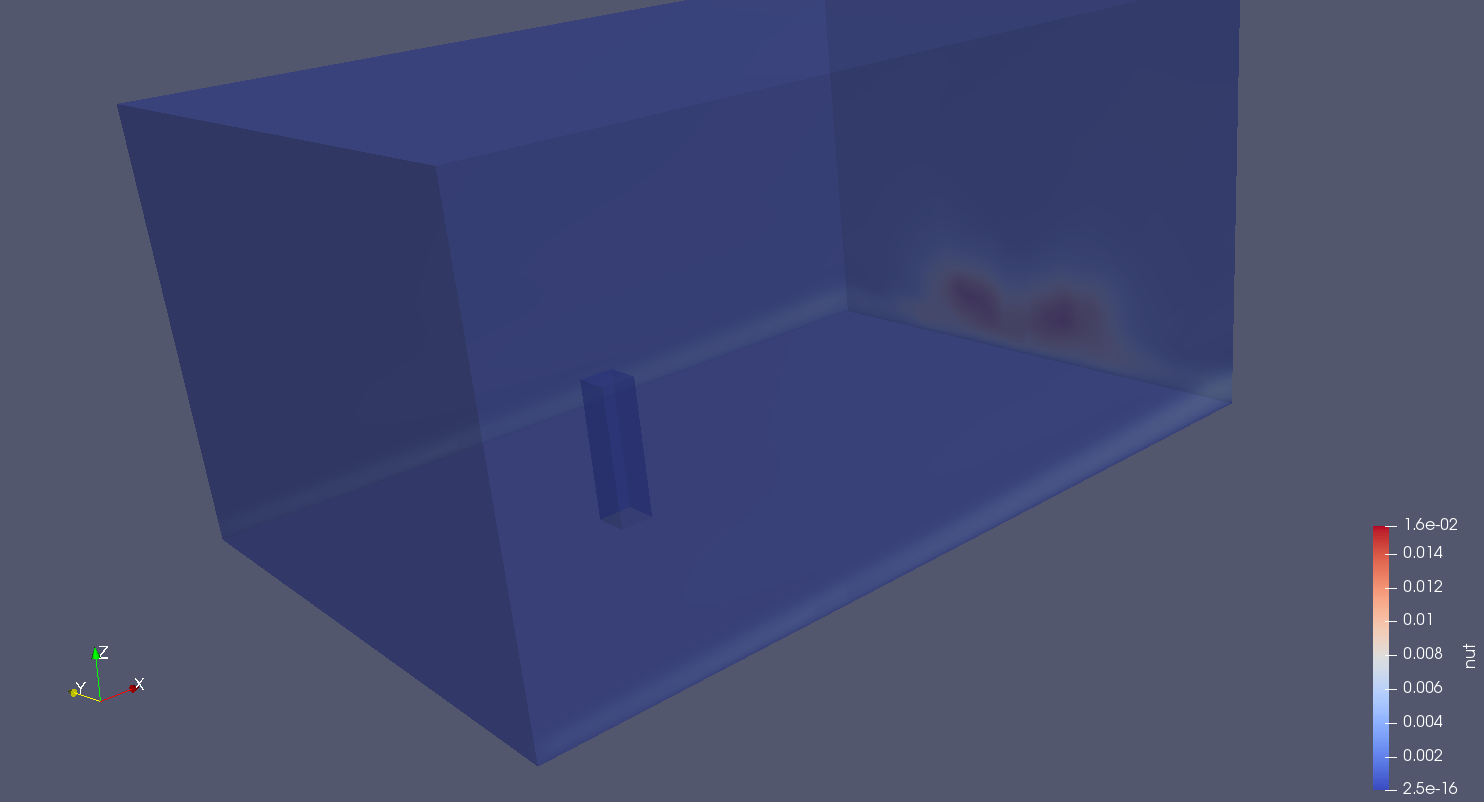
\includegraphics[width=0.45\textwidth]{figs/sqcyl/nut.png}}}%
    \caption{}%
    \label{fig:sqcyl}%
\end{figure}

\begin{figure}[H]%
    \centering
    \subfloat[\centering $I_1$]{{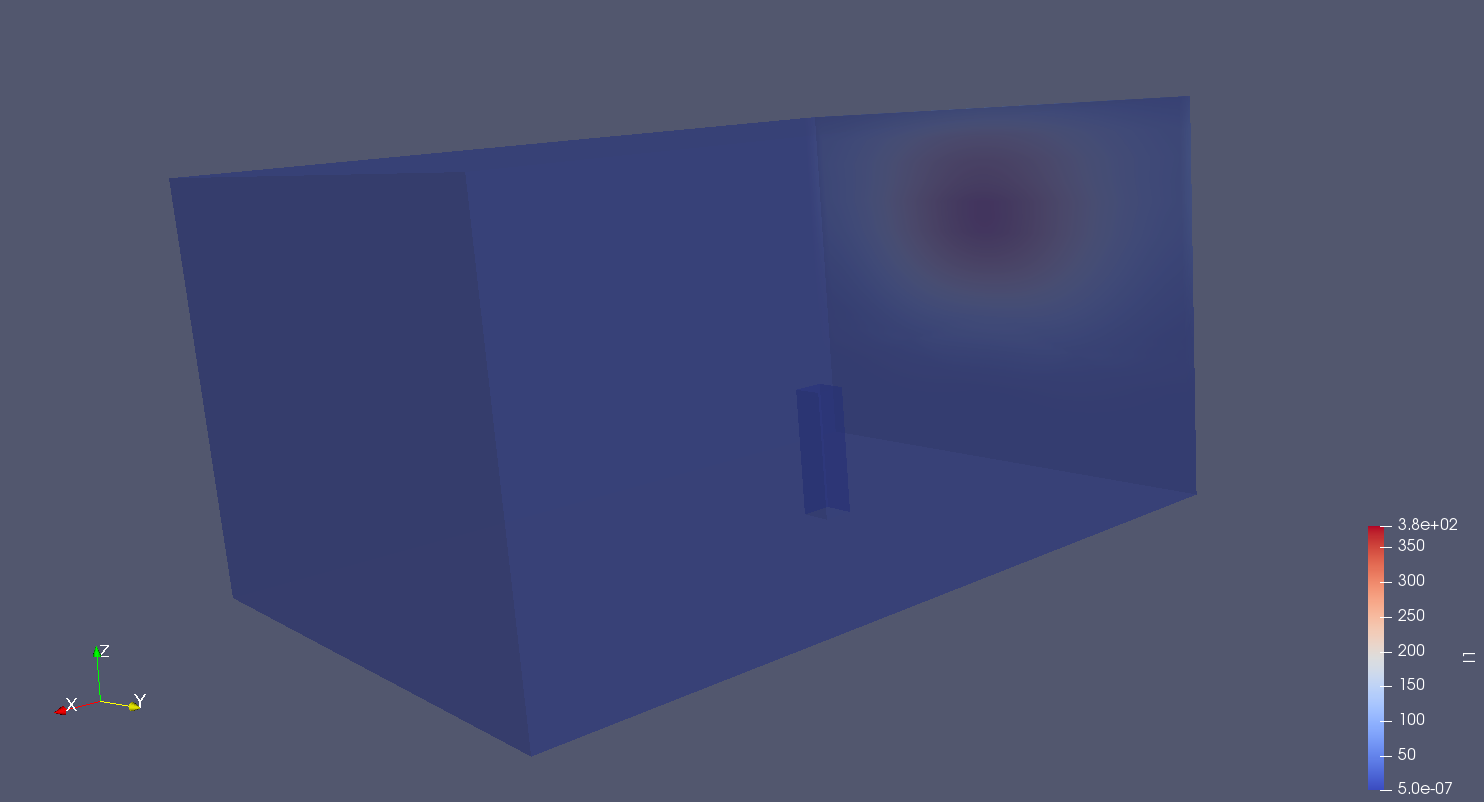
\includegraphics[width=0.45\textwidth]{figs/sqcyl/I1.png}}}%
    \qquad
    \subfloat[\centering $R$ term]{{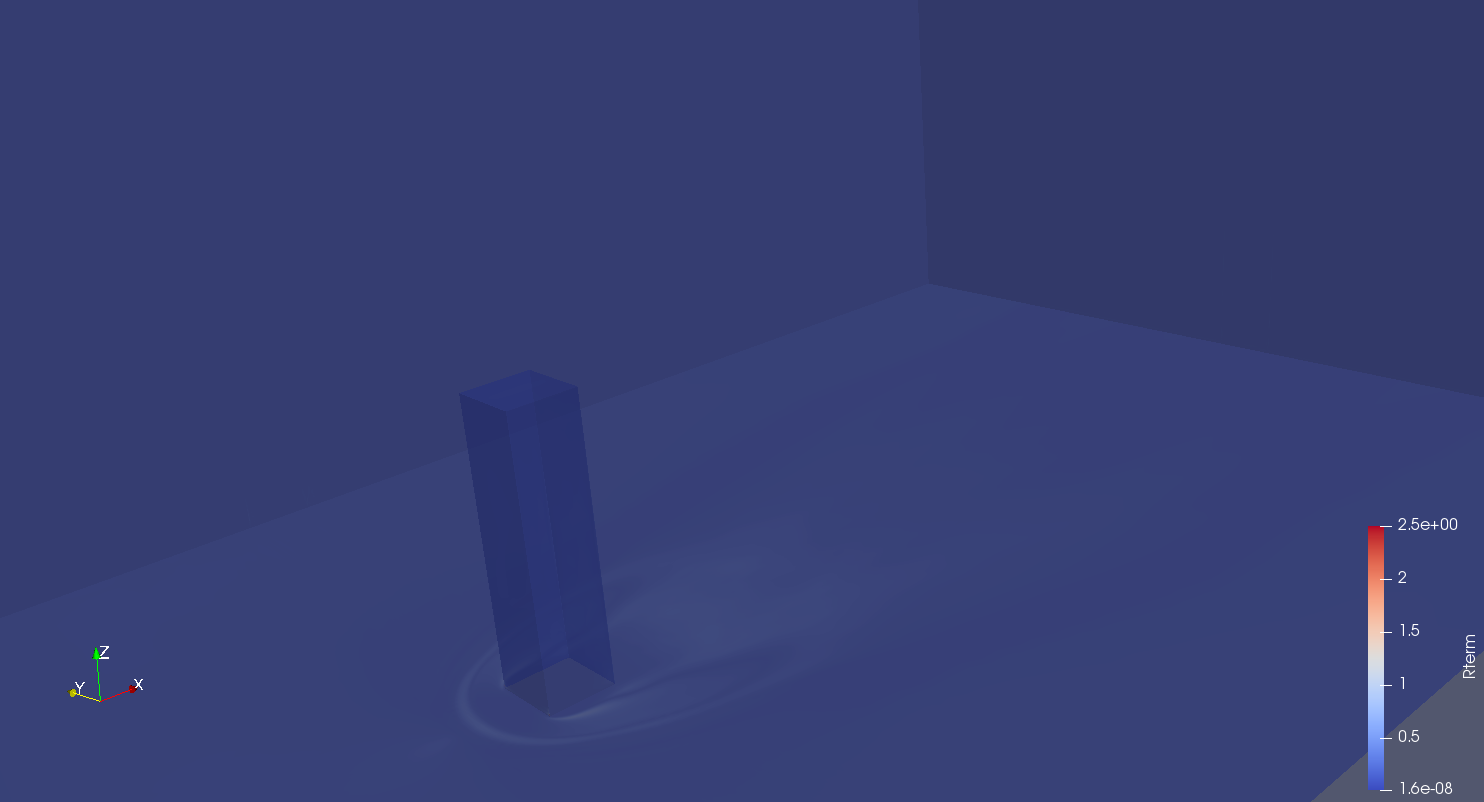
\includegraphics[width=0.45\textwidth]{figs/sqcyl/Rterm.png}}}%
    \caption{}%
    \subfloat[\centering $R$ term norm]{{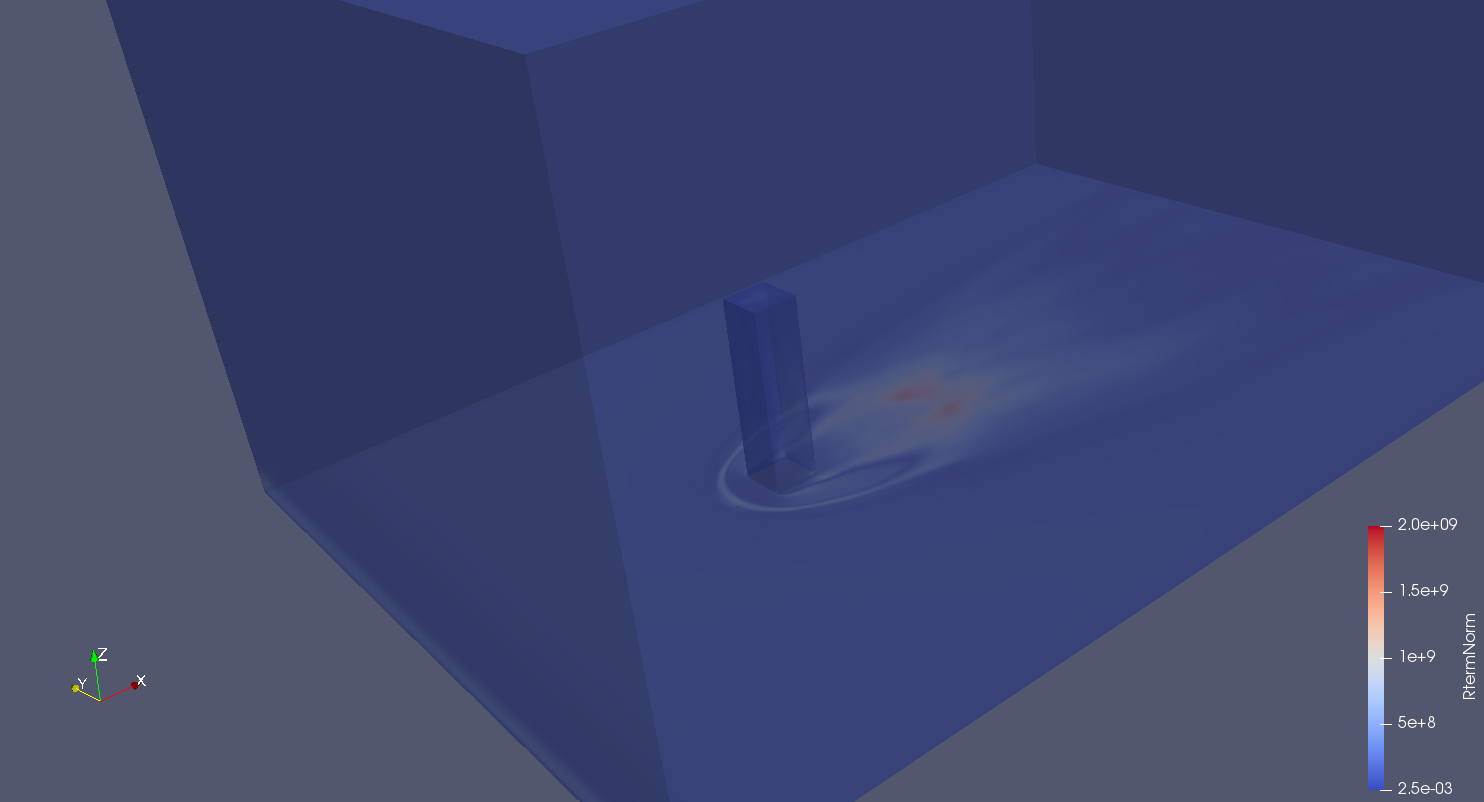
\includegraphics[width=0.45\textwidth]{figs/sqcyl/RtermNorm.png}}}%
    \qquad
    \subfloat[\centering $T_1$ magnitude]{{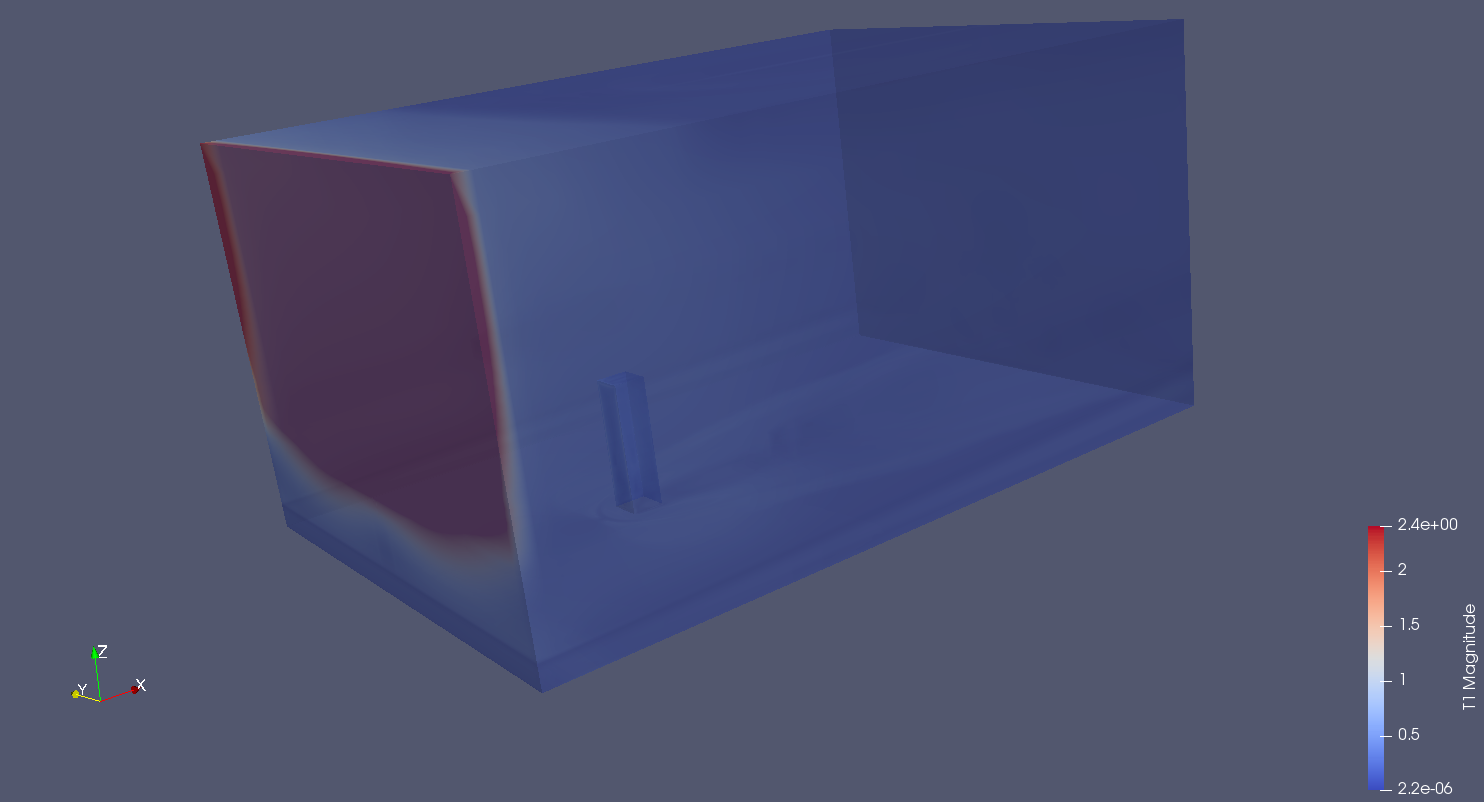
\includegraphics[width=0.45\textwidth]{figs/sqcyl/T1_magn.png}}}%
    \caption{}%
    \subfloat[\centering $T_2$ magnitude]{{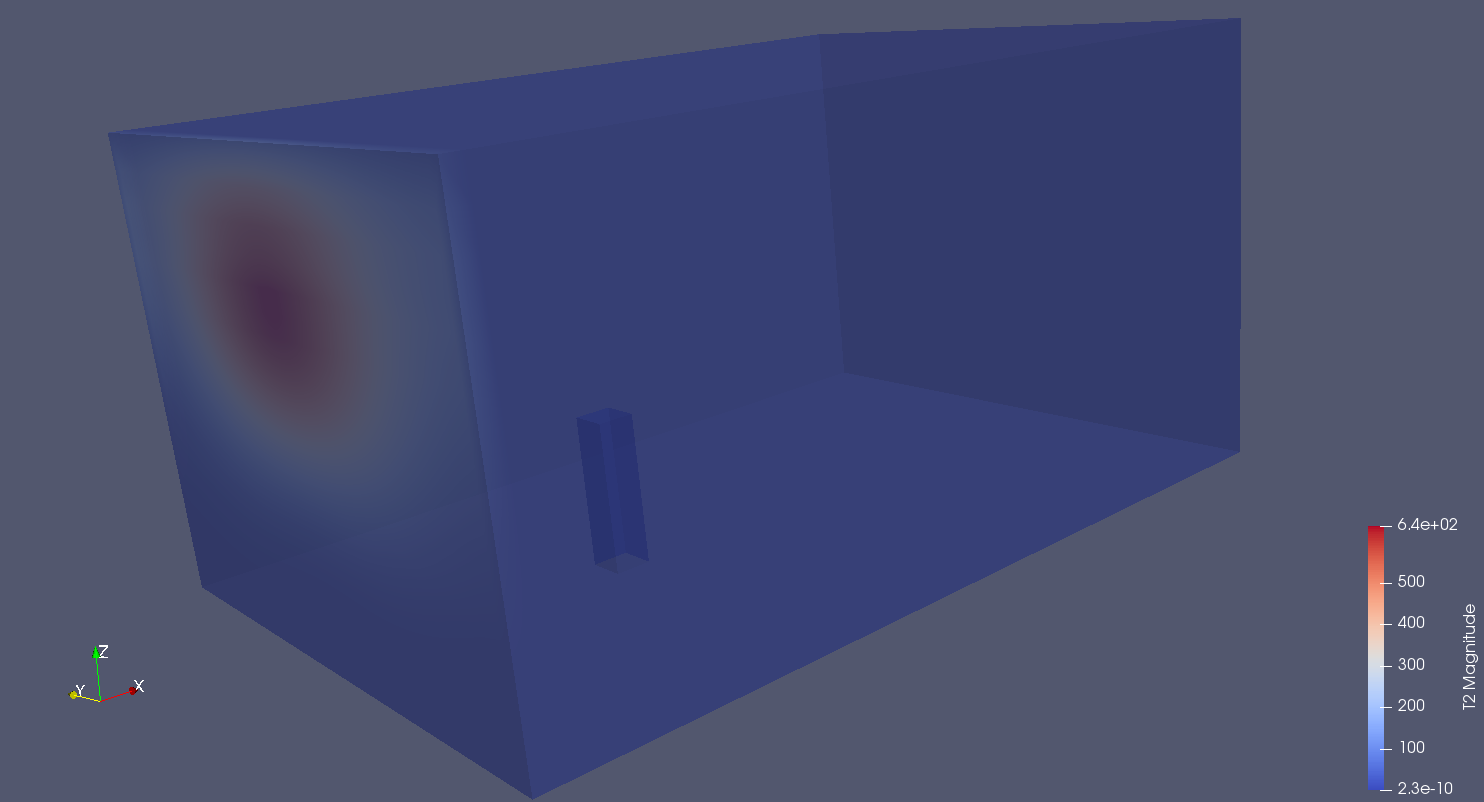
\includegraphics[width=0.45\textwidth]{figs/sqcyl/T2_magn.png}}}%
    \qquad
    \subfloat[\centering $R_{res}$]{{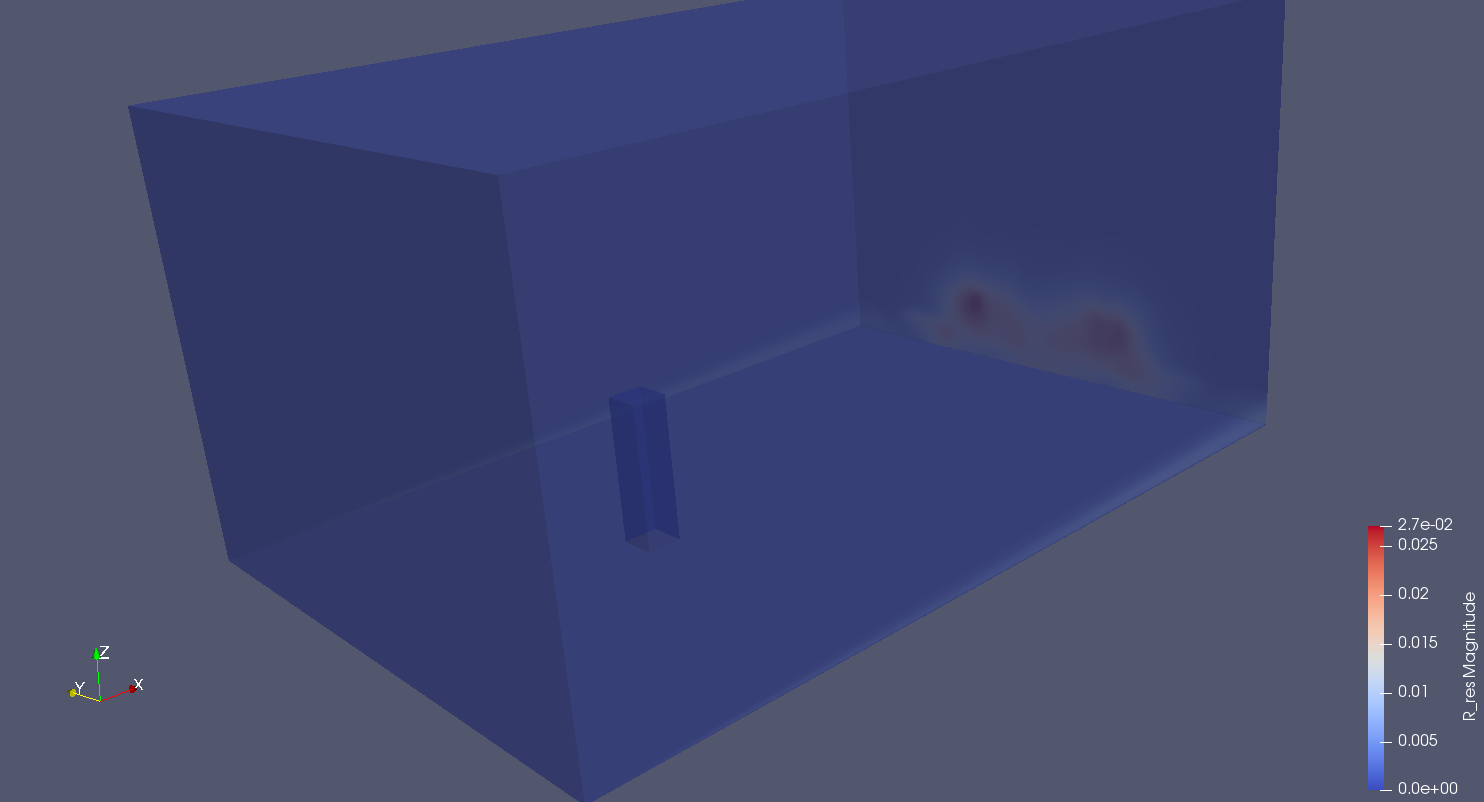
\includegraphics[width=0.45\textwidth]{figs/sqcyl/R_res.png}}}%
    \caption{}%
    \subfloat[\centering $R_{sgs}$]{{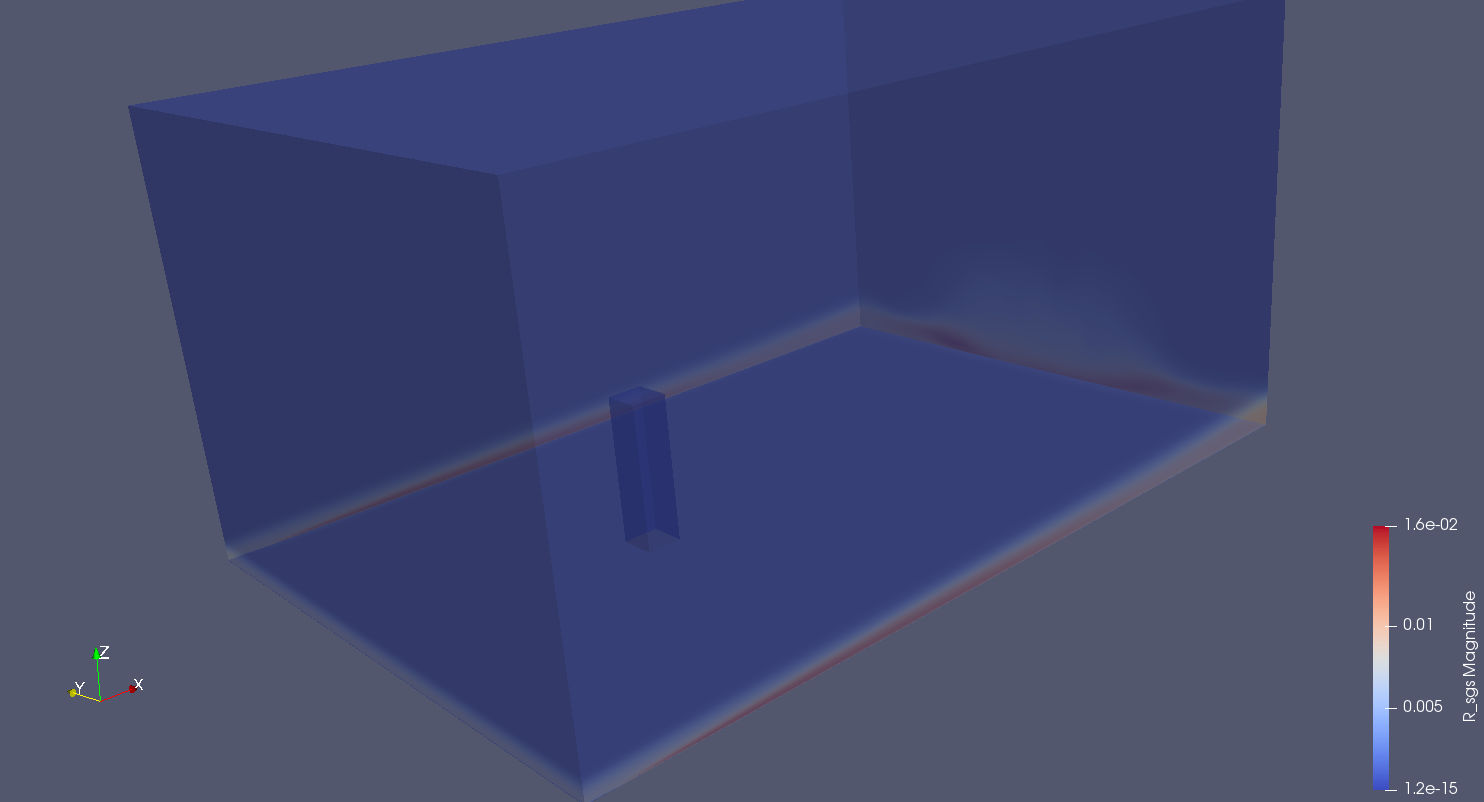
\includegraphics[width=0.45\textwidth]{figs/sqcyl/R_sgs.png}}}%
    \qquad
    \subfloat[\centering $R_{tot}$]{{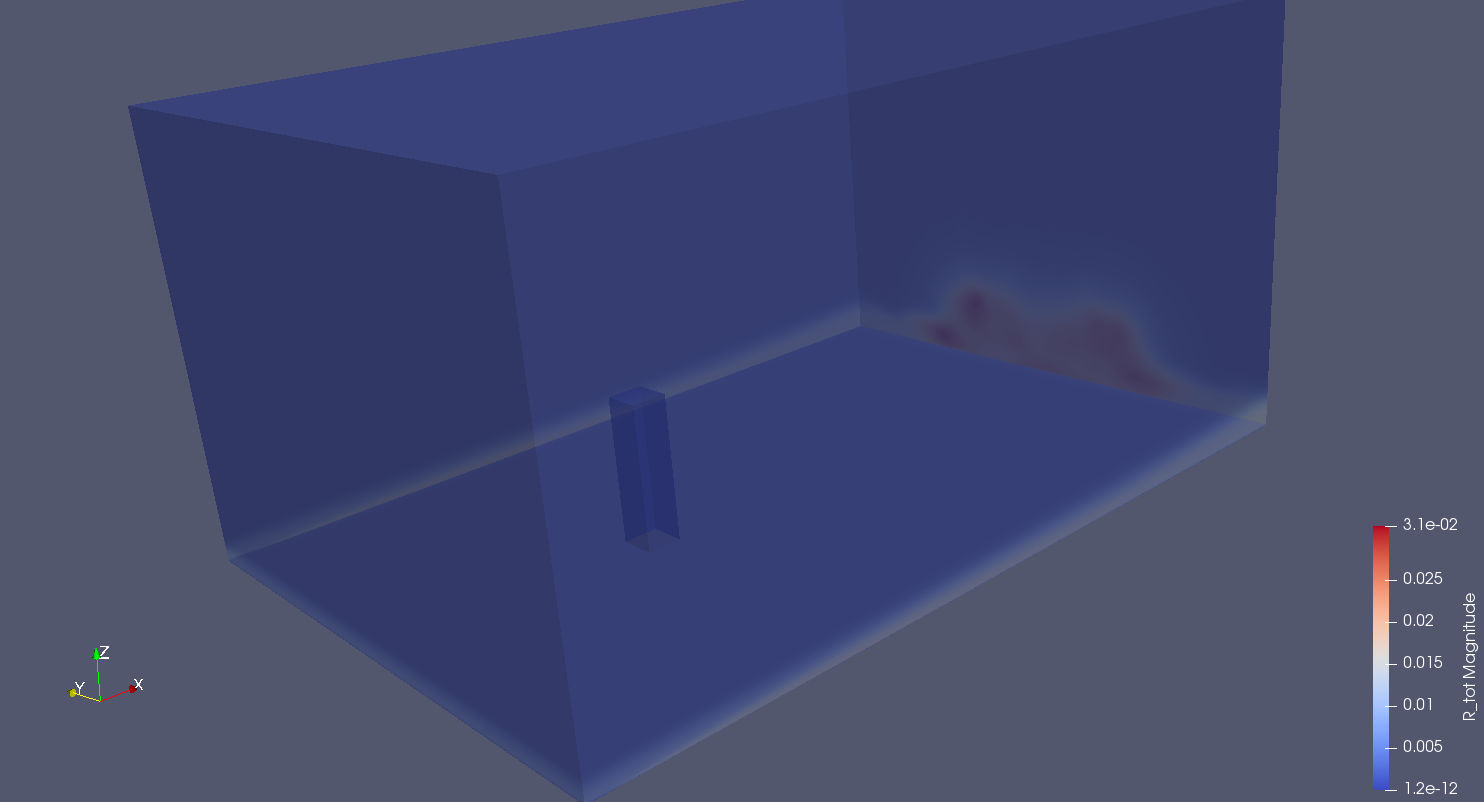
\includegraphics[width=0.45\textwidth]{figs/sqcyl/R_tot.png}}}%
    \caption{Some fields for a wall-mounted squared cylinder testcase.}%
    \label{fig:sqcyl}%
\end{figure}

\begin{figure}[H]%
    \centering
    \subfloat[\centering OF]{{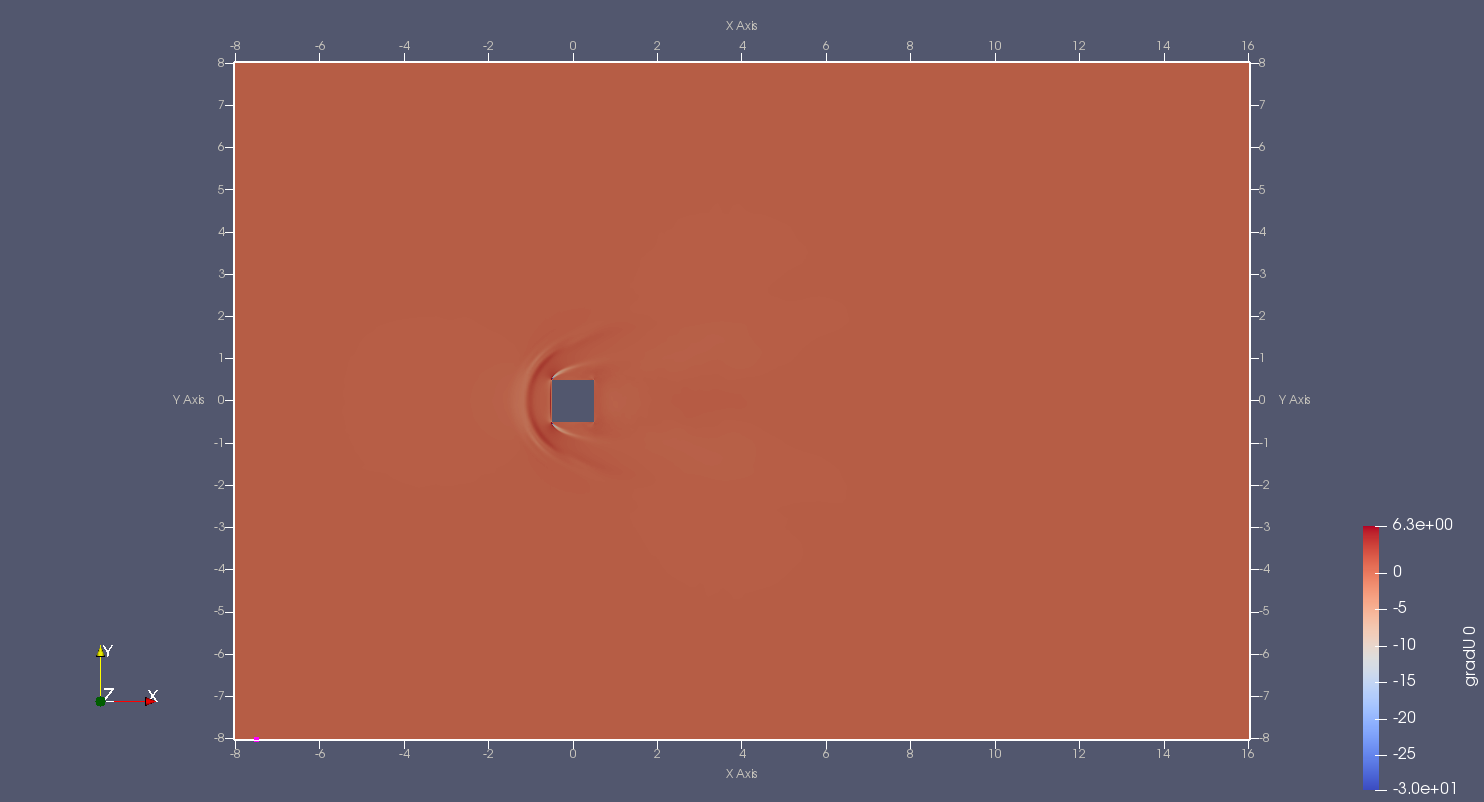
\includegraphics[width=0.45\textwidth]{figs/sqcyl/gradU/gradU0.png}}}%
    \qquad
    \subfloat[\centering R]{{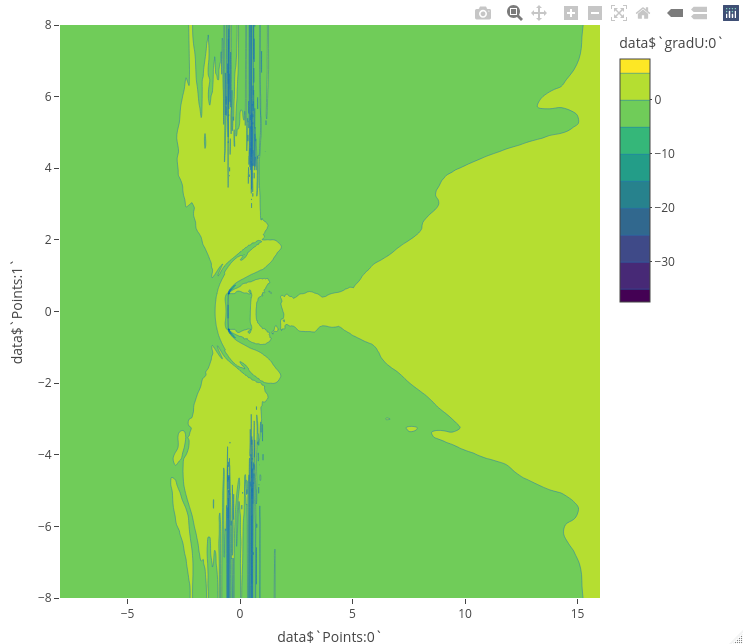
\includegraphics[width=0.3\textwidth]{figs/sqcyl/gradU_R/gradU0.png}}}%
    \caption{gradU0}%
    \subfloat[\centering OF]{{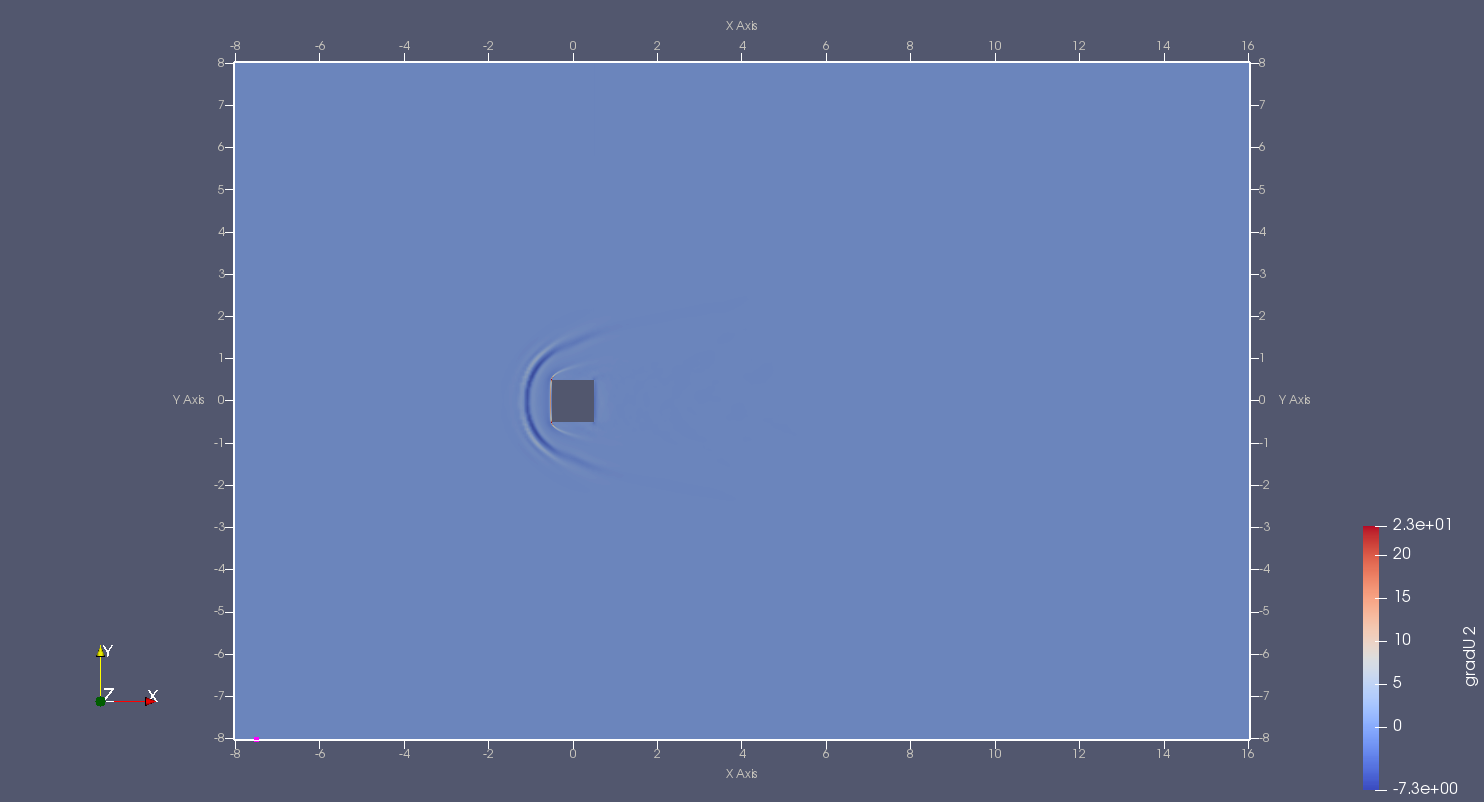
\includegraphics[width=0.45\textwidth]{figs/sqcyl/gradU/gradU2.png}}}%
    \qquad
    \subfloat[\centering R]{{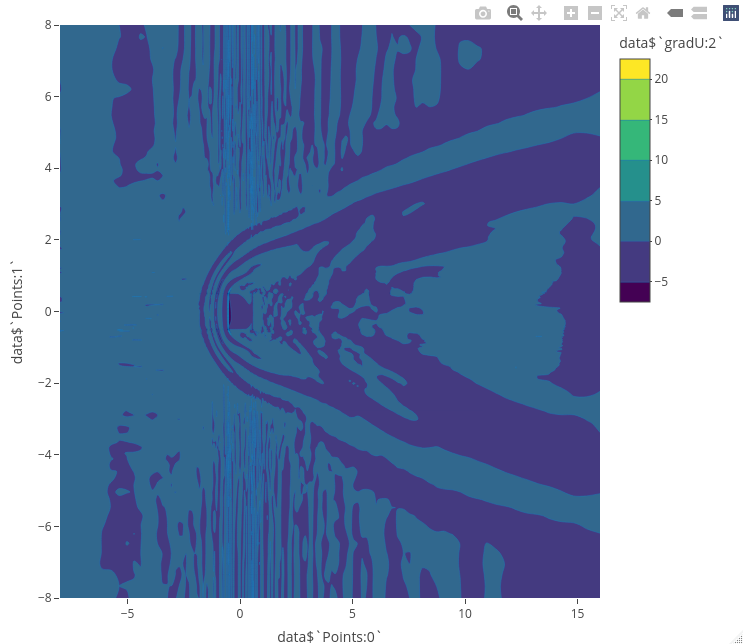
\includegraphics[width=0.3\textwidth]{figs/sqcyl/gradU_R/gradU2.png}}}%
    \caption{gradU2}%
    \subfloat[\centering OF]{{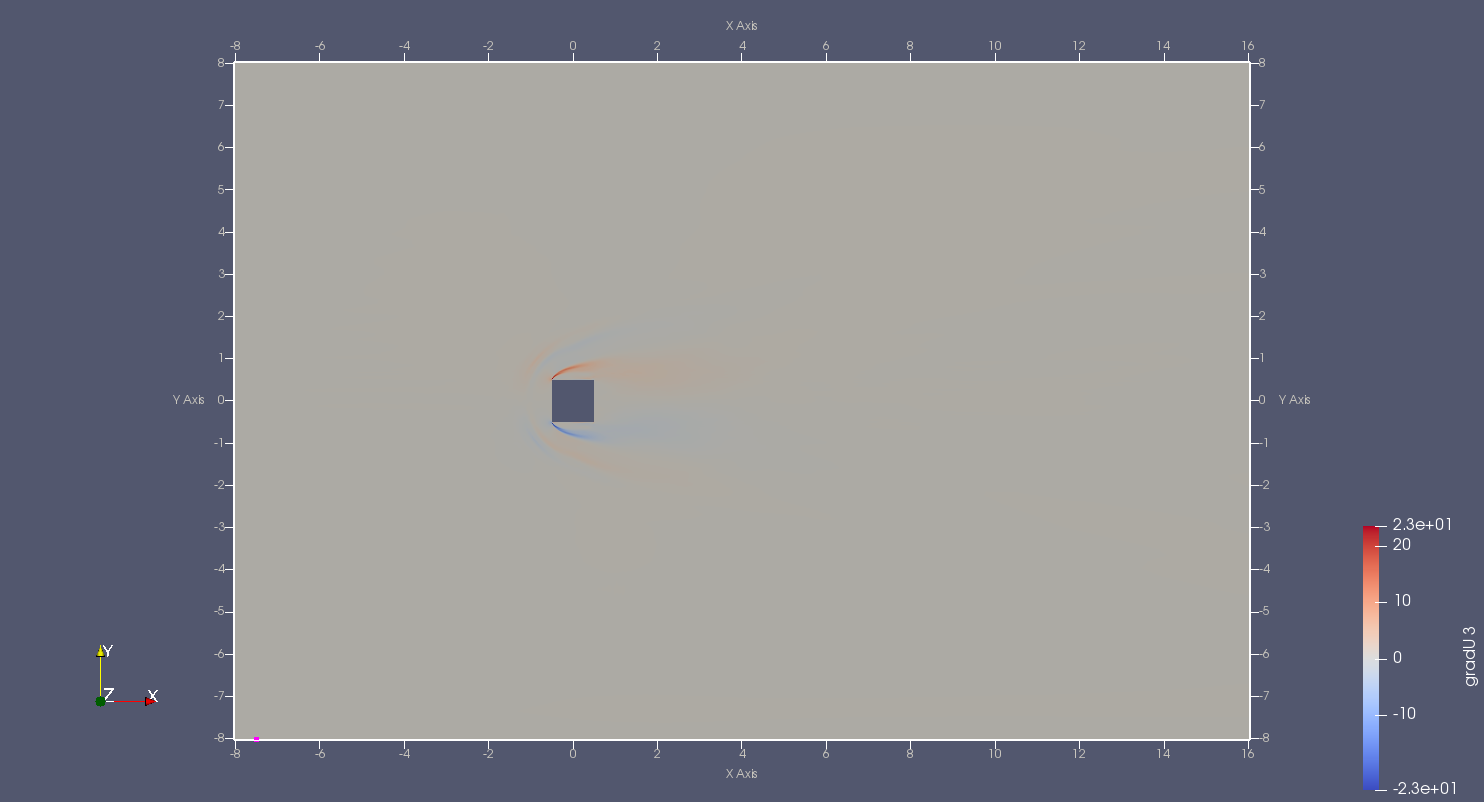
\includegraphics[width=0.45\textwidth]{figs/sqcyl/gradU/gradU3.png}}}%
    \qquad
    \subfloat[\centering R]{{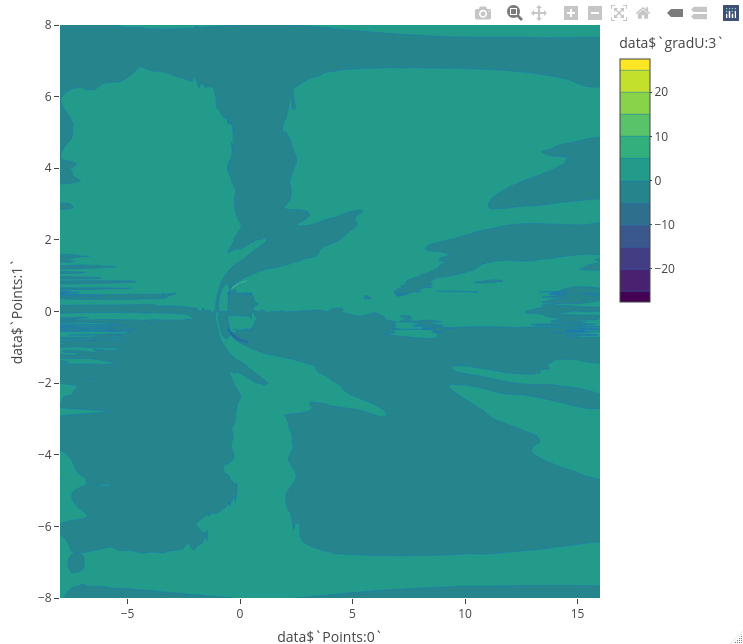
\includegraphics[width=0.3\textwidth]{figs/sqcyl/gradU_R/gradU3.png}}}%
    \caption{gradU3}%
    \subfloat[\centering OF]{{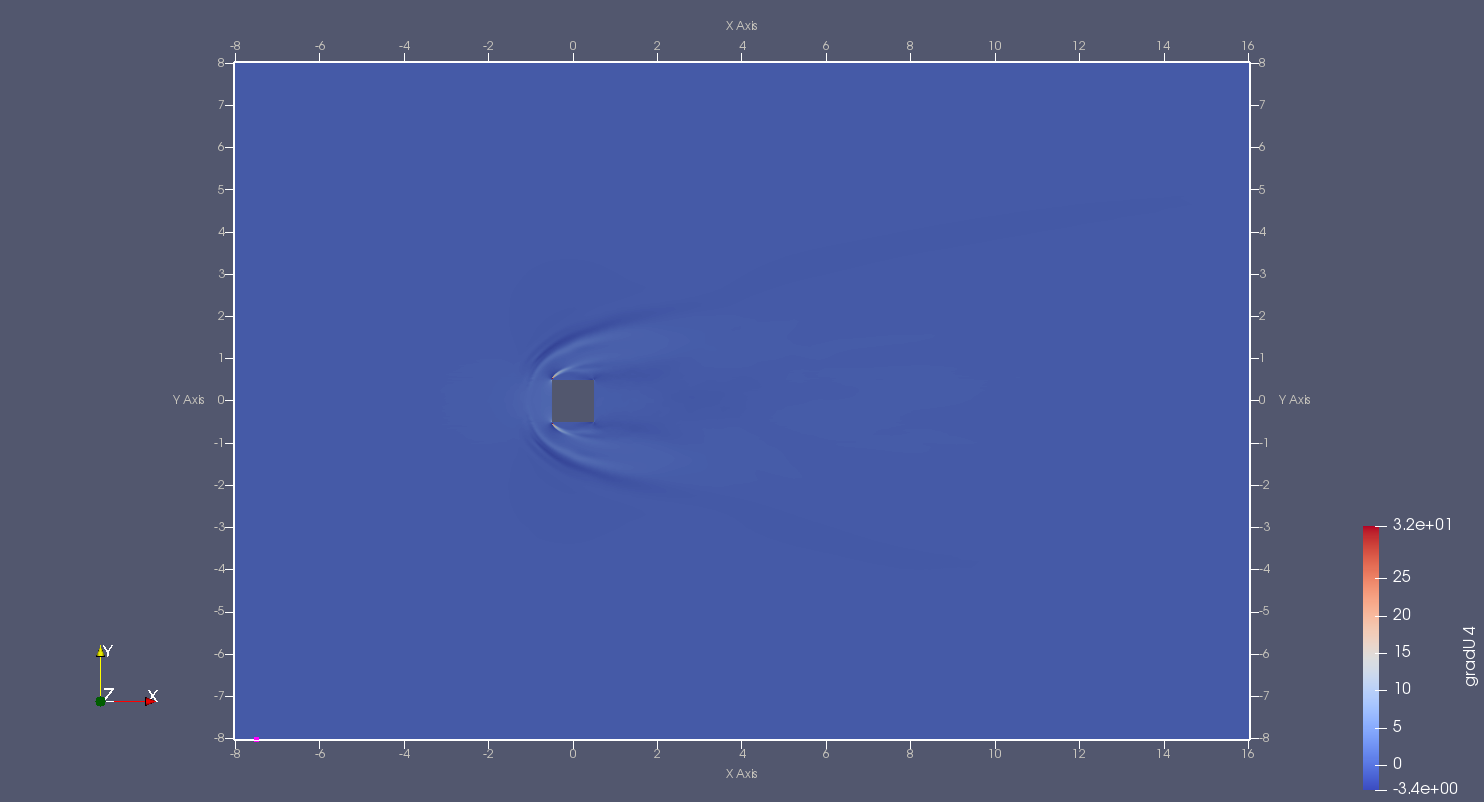
\includegraphics[width=0.45\textwidth]{figs/sqcyl/gradU/gradU4.png}}}%
    \qquad
    \subfloat[\centering R]{{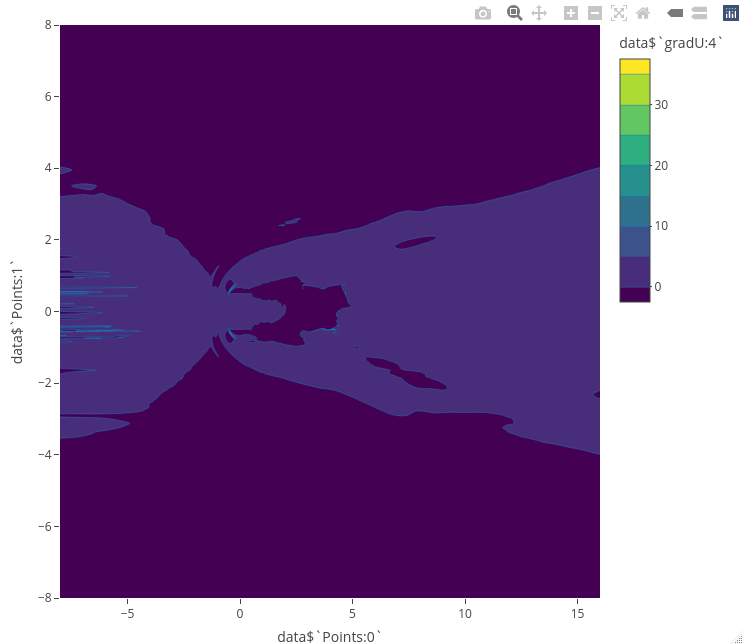
\includegraphics[width=0.3\textwidth]{figs/sqcyl/gradU_R/gradU4.png}}}%
    \caption{gradU4}%
    \label{fig:sqcyl:gradu}%
\end{figure}

\begin{figure}[H]%
    \centering
    \subfloat[\centering OF]{{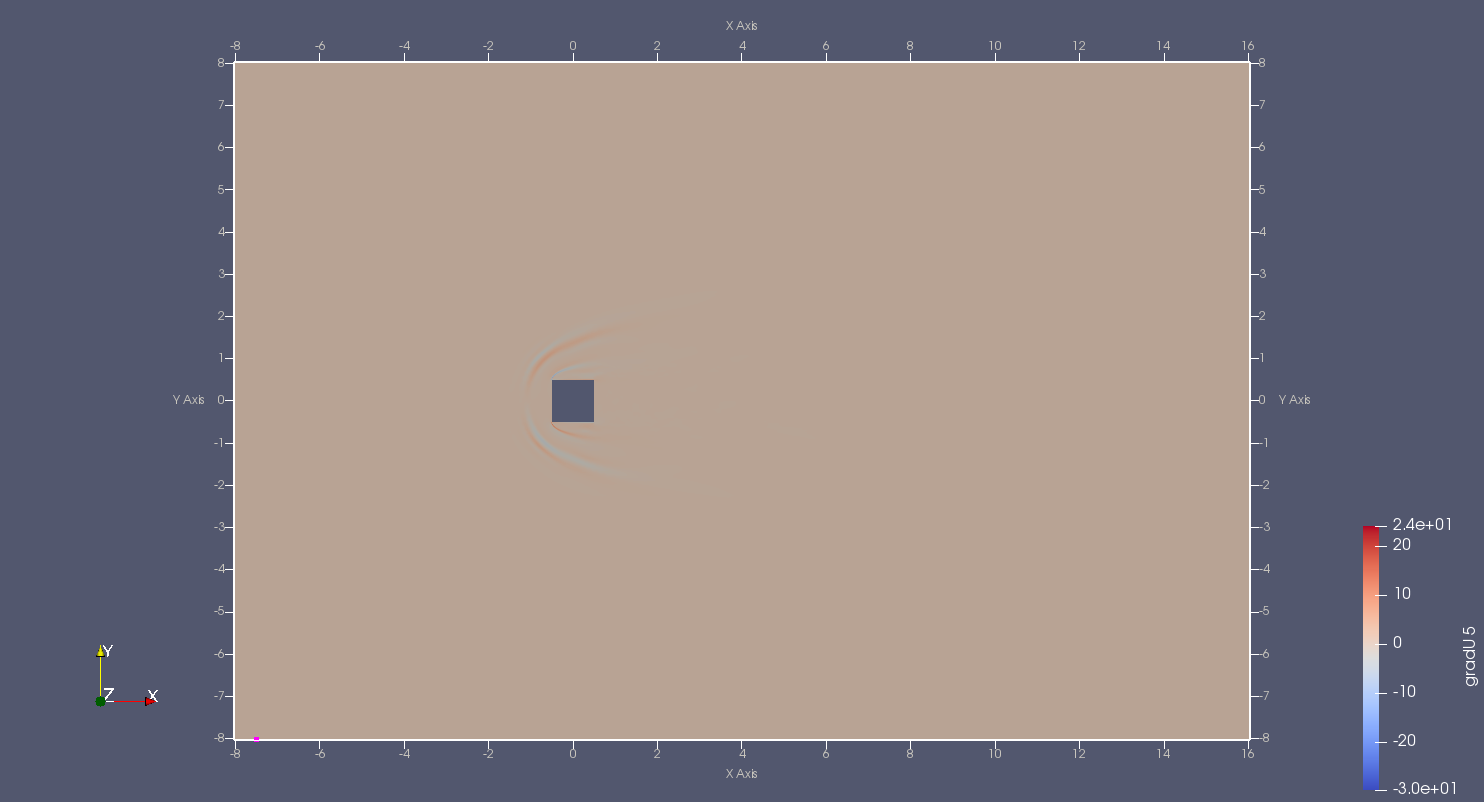
\includegraphics[width=0.45\textwidth]{figs/sqcyl/gradU/gradU5.png}}}%
    \qquad
    \subfloat[\centering R]{{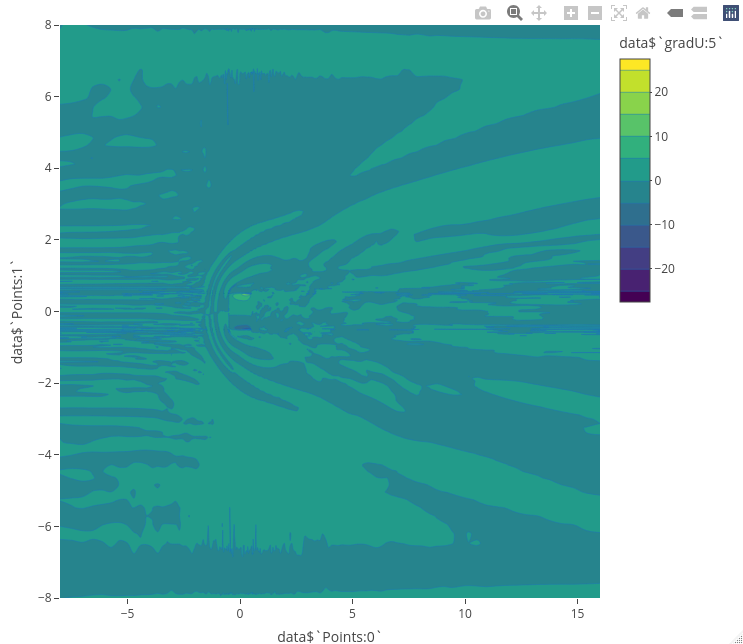
\includegraphics[width=0.3\textwidth]{figs/sqcyl/gradU_R/gradU5.png}}}%
    \caption{gradU5}%
    \subfloat[\centering OF]{{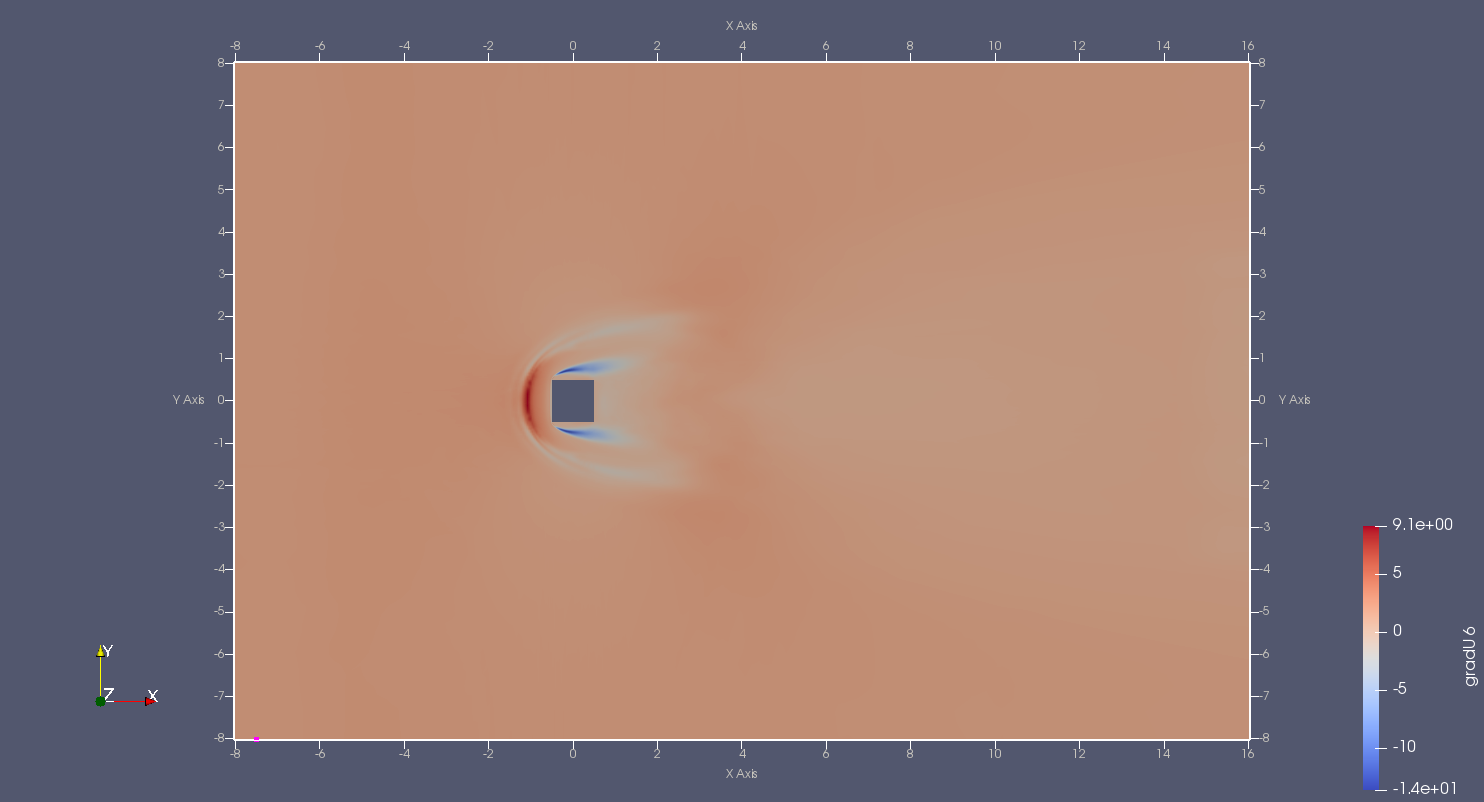
\includegraphics[width=0.45\textwidth]{figs/sqcyl/gradU/gradU6.png}}}%
    \qquad
    \subfloat[\centering R]{{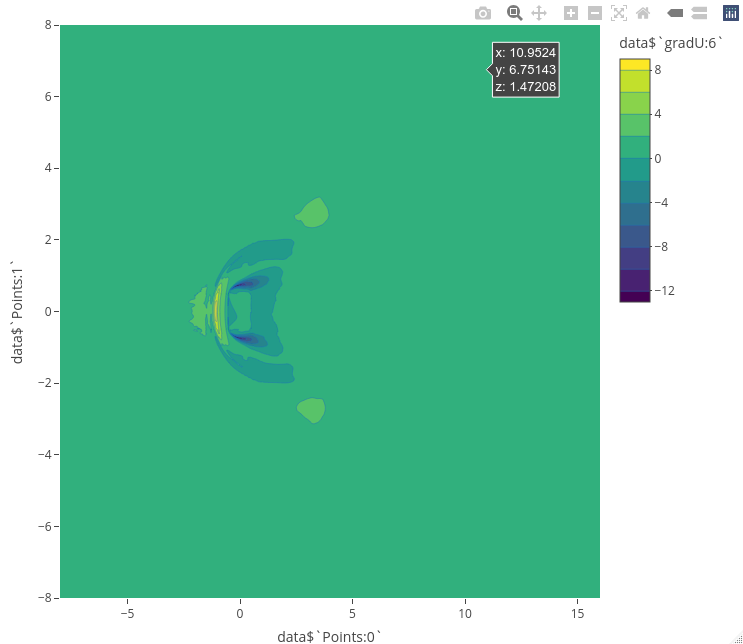
\includegraphics[width=0.3\textwidth]{figs/sqcyl/gradU_R/gradU6.png}}}%
    \caption{gradU6}%
    \subfloat[\centering OF]{{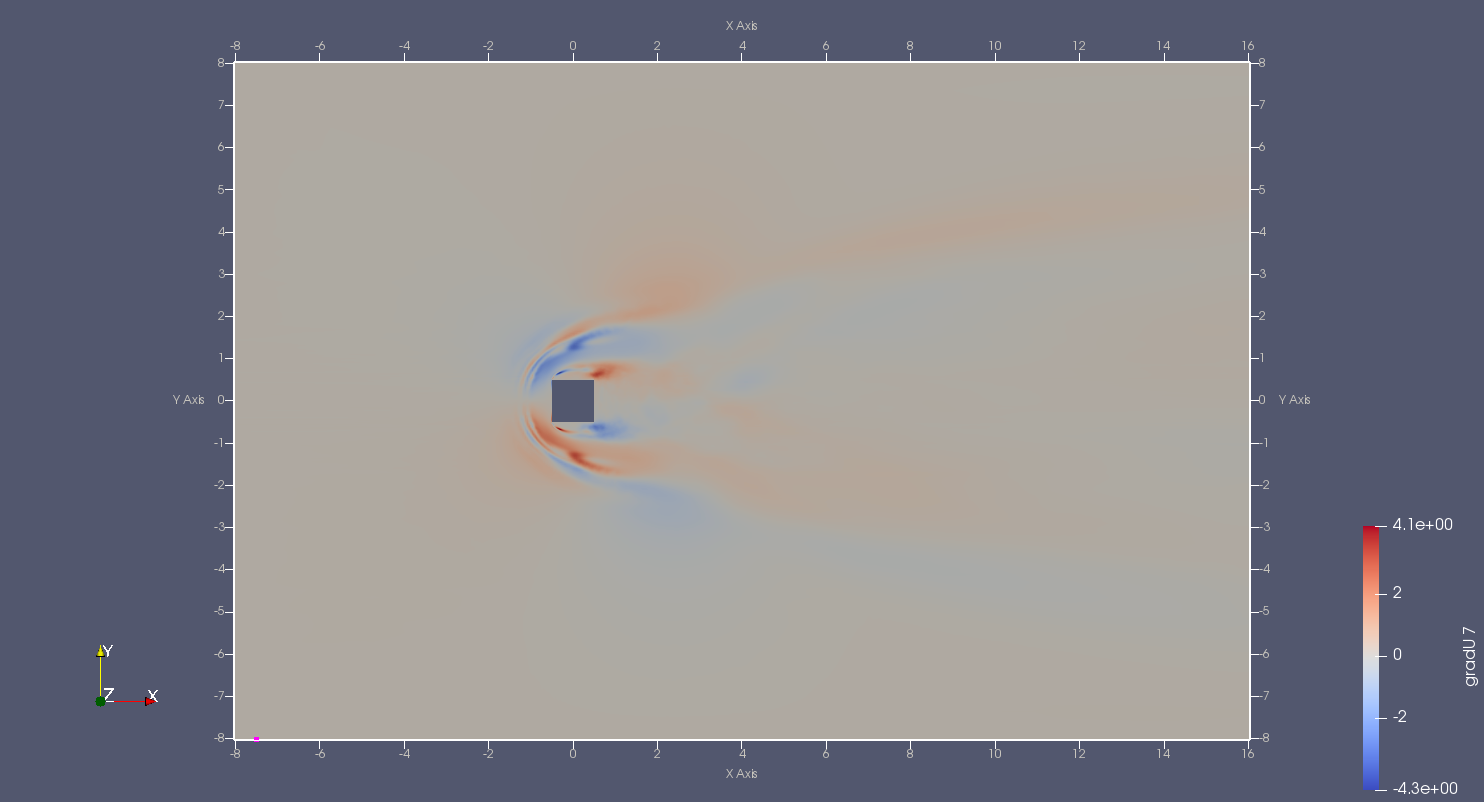
\includegraphics[width=0.45\textwidth]{figs/sqcyl/gradU/gradU7.png}}}%
    \qquad
    \subfloat[\centering R]{{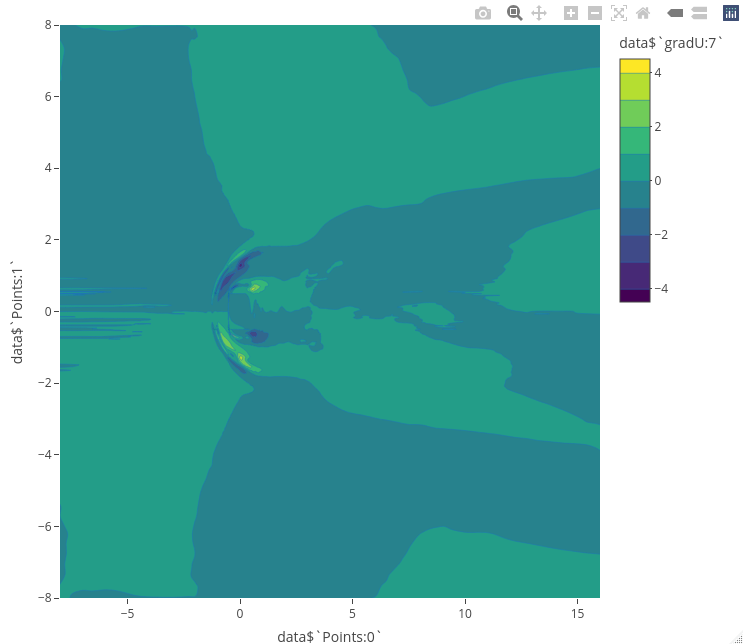
\includegraphics[width=0.3\textwidth]{figs/sqcyl/gradU_R/gradU7.png}}}%
    \caption{gradU7}%
    \subfloat[\centering OF]{{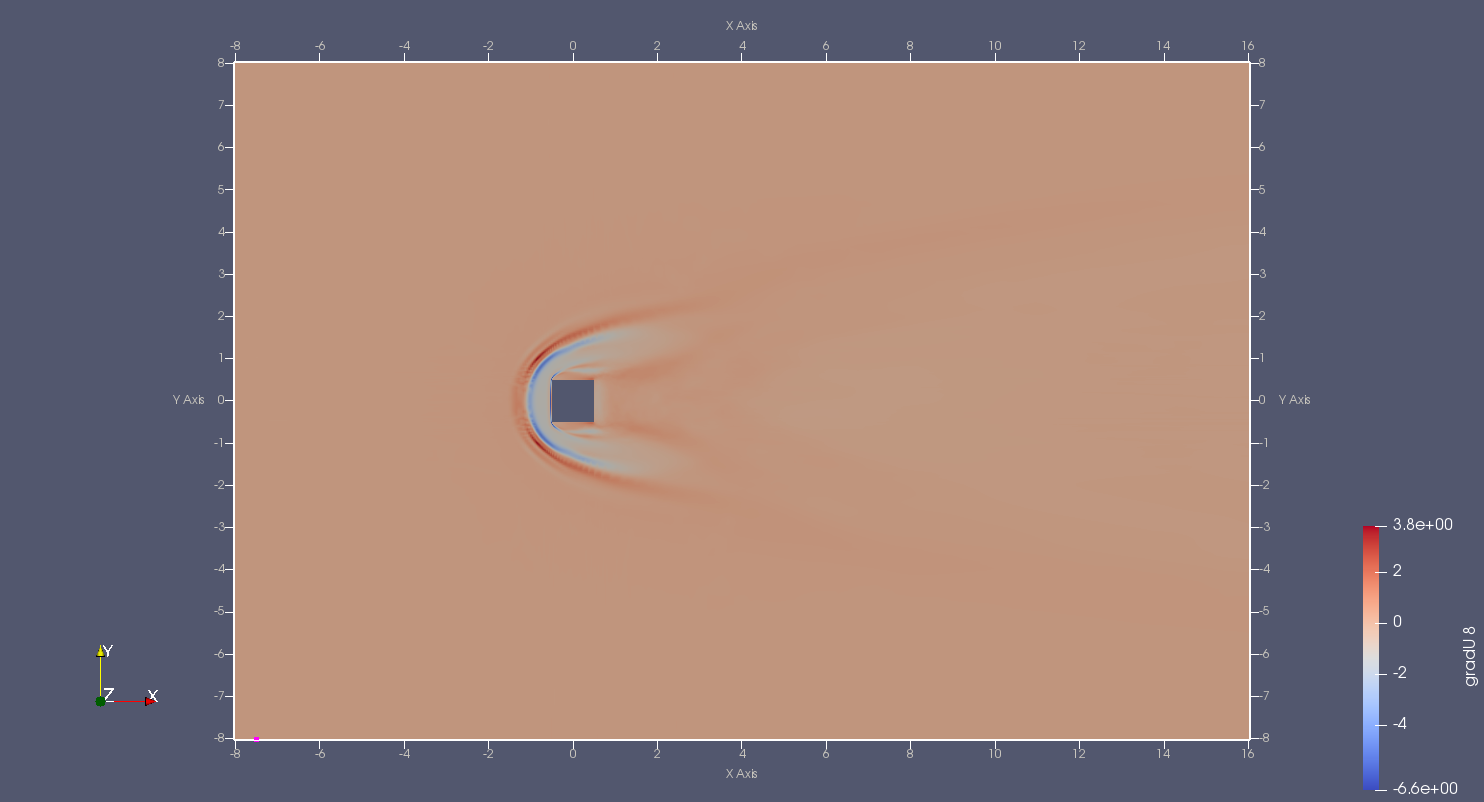
\includegraphics[width=0.45\textwidth]{figs/sqcyl/gradU/gradU8.png}}}%
    \qquad
    \subfloat[\centering R]{{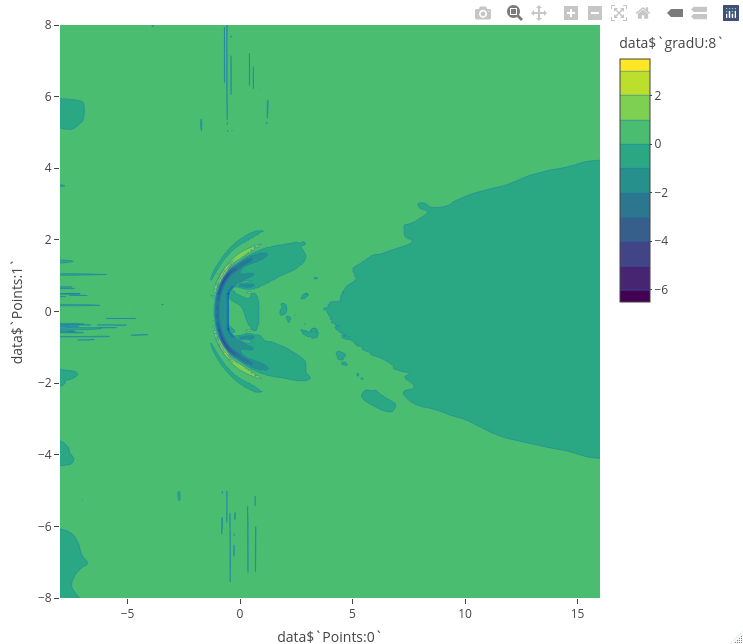
\includegraphics[width=0.3\textwidth]{figs/sqcyl/gradU_R/gradU8.png}}}%
    \caption{gradU8}%
    \label{fig:sqcyl:gradu}%
\end{figure}

\begin{figure}[H]%
    \centering
    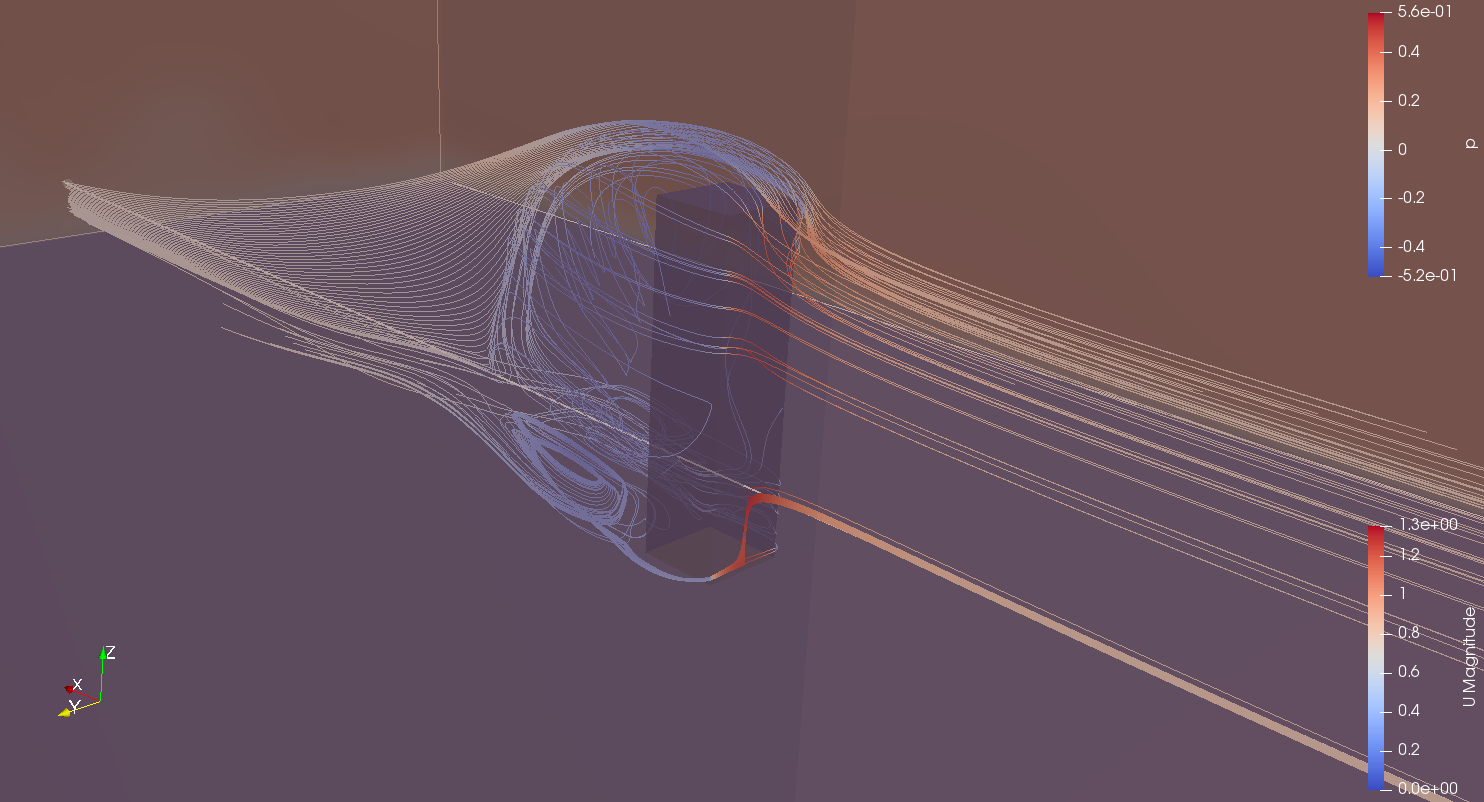
\includegraphics[width=0.9\textwidth]{figs/streamlines.png}
    \caption{Streamlines around a  a wall-mounted square cylinder. The velocity field is shown and the streamlines are coloured as the pressure field.}
    \label{fig:streamlines}%
\end{figure}

\begin{figure}[H]%
    \centering
    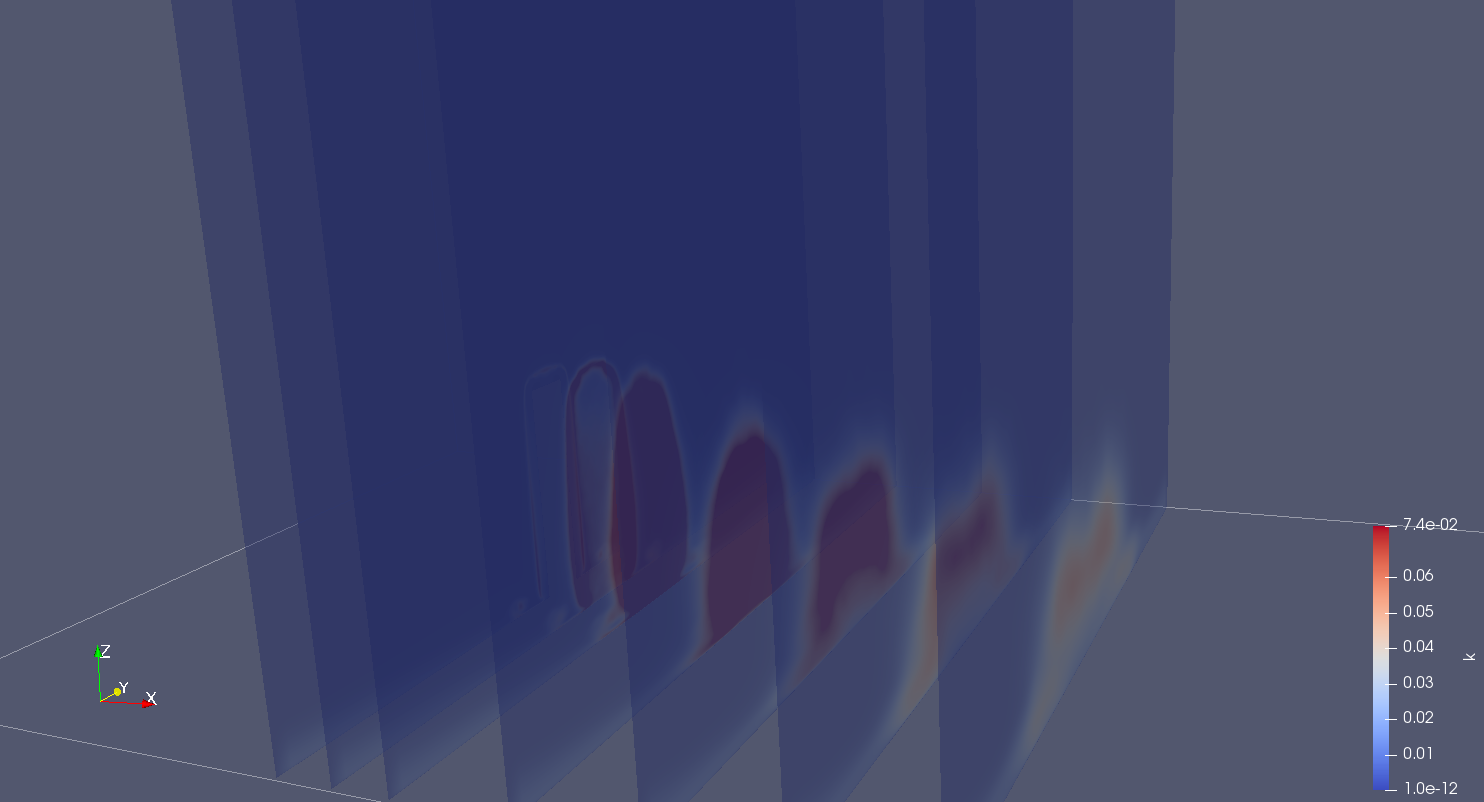
\includegraphics[width=0.9\textwidth]{figs/sqcyl/gradU/k_clips.png}
    \caption{Clips of the turbulence kinetic energy field $k$ for the wall-mounted square cylinder. Extractions planes at x = 0, 1, 2, 4, 6, 8, 10 m.}
    \label{fig:k_clips}%
\end{figure}

%\begin{figure}[H]%
%    \centering
%    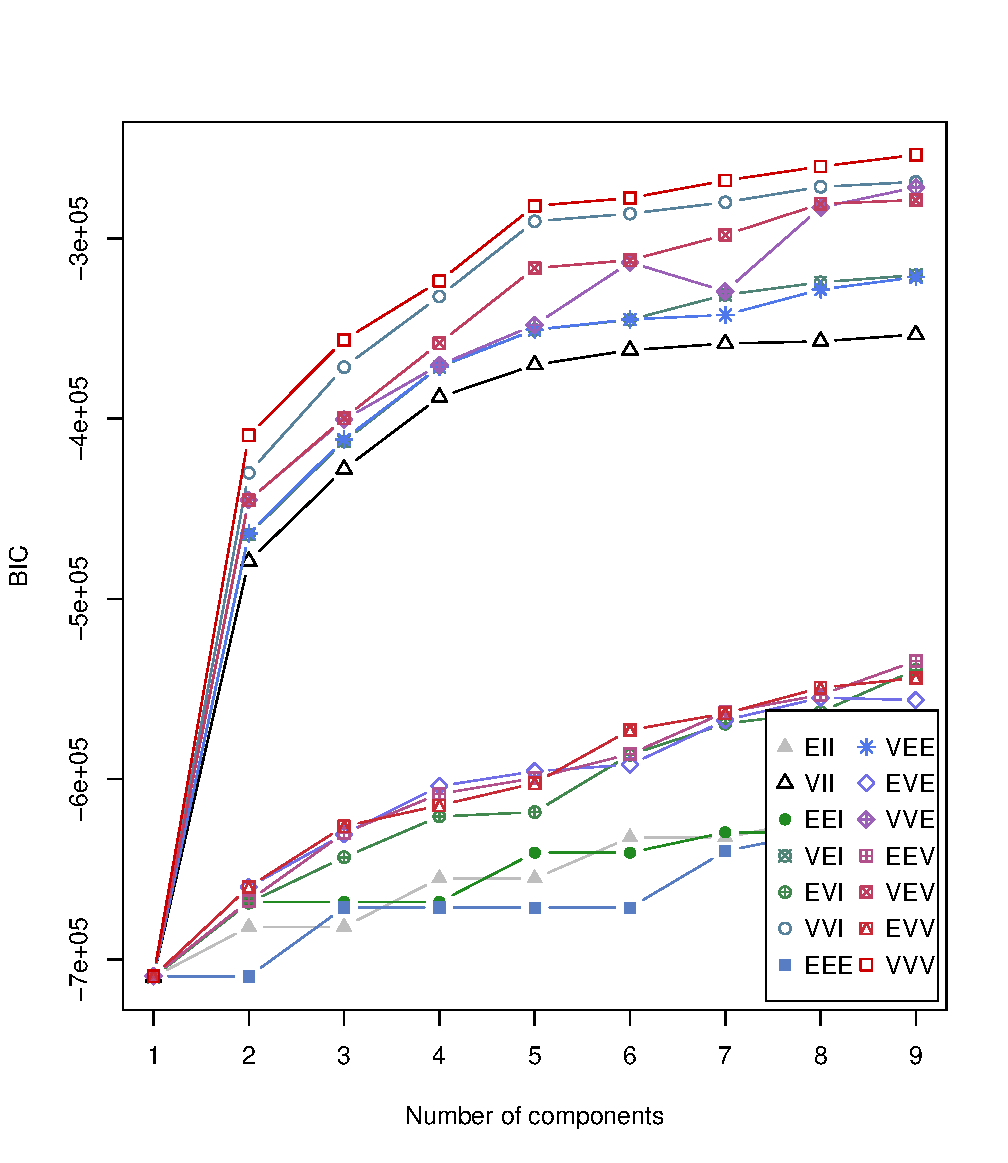
\includegraphics[width=0.9\textwidth]{figs/sqcyl/gradU_R/cluster/BIC.pdf}
%    \caption{BIC.}
%    \label{fig:bic}%
%\end{figure}
%\begin{figure}[H]%
%    \centering
%    \includegraphics[width=0.9\textwidth]{figs/sqcyl/gradU_R/cluster/classification.pdf}
%    \caption{Classification}
%    \label{fig:classification}%
%\end{figure}
%\begin{figure}[H]%
%    \centering
%    \includegraphics[width=0.9\textwidth]{figs/sqcyl/gradU_R/cluster/clusters_gradU6_7_8.pdf}
%    \caption{clusters}
%    \label{fig:clusters}%
%\end{figure}
%\begin{figure}[H]%
%    \centering
%    \includegraphics[width=0.9\textwidth]{figs/sqcyl/gradU_R/cluster/num_clusters.pdf}
%    \caption{Number of clusters}
%    \label{fig:numclusters}%
%\end{figure}

%\chapter{Data-driven turbulence modeling enhanced by prototype selection}
%\section{Introduction}
%
In this report we document our efforts to develop and test an authentication methodology for
machine-learned (ML) models of physical phenomena. By authentication, we imply the ability to
determine two separate qualities of a ML model. The first refers to the ability to identify the types of
physics the ML model represents, and thus qualify the model i.e., demarcate the scenarios where the ML
model can and cannot be used. The second quality is the ability to ascertain the degree to which the ML
model, as trained, adheres to the laws of physics. The methodology aims at being general but will be tested on a data-driven GEP-enhanced turbulence closure of the Reynolds-Averaged Navier Stokes (RANS) equation, the de-facto workhorse of turbulent flow simulations in engineering settings.

Engineering models/simulators most often do not explicitly resolve fine-scale physical phenomena due to
computational expense; instead, they use empirical models called "closures" or "constitutive
models". Over the last few years, these closures have been fashioned as machine-learned models trained on data assembled from a handful number of high-fidelity simulations of configurations of intermediate
complexity (for which high-fidelity simulations are tractable). These ML closures have delivered
enhanced accuracy and have captured physical phenomena that have eluded conventional closures. However, RANS modeling deficiencies, particularly for some type of flows, are very well-known. 
This motivated several researchers to investigate possible alternatives to improve RANS closures. In~\cite{Sandberg2022} a review of flow physics simulations where RANS modeling was improved by adopting Gene Programming Expression (GEP) paradigm was reported. At the end of the paper, the authors comment about the possibility of developing a "universal turbulence closure model"  or more realistically the idea of realizing some kind of "filter" or "selector", which would automatically choose the most appropriate model for specific flow regions.

In this report, such idea will be further pursued and developed. In this regard, having a method that can quantify the quality of closure models i.e., check their adherence to physics theory, and to qualify them i.e., demarcate the situations where they can be used appears to be an important step in this direction and is the objective of our authentication methodology.

We assume that the database could be decomposed into partitions i.e., a subset that encode a particular type of physics. In addition, we assume that each partition can be summarized with a handful of examples (the "prototypes") that can be analyzed so that we may characterize the physics in each partition.

The research questions are:
\begin{enumerate}
    \item A dataset can be partitioned via clustering but how does one assemble a feature-space while doing so? One can embed physics knowledge by proposing a large number of physical quantities that could serve as elements of the feature-space, but only a few are probably required. How does one determine the useful subset of the over-complete dictionary of potential features?
    \item How does one select prototypes? We would like to keep them as few as possible, then, what degree of summarization can we achieve and what are the metrics that quantify the quality of a prototype set? Note that prototypes need to cover the entire partition and there is no requirement that their selection reflect the density of examples in the partition.
\end{enumerate}
%
We test our authentication methodology using a GEP-enhanced closure models for the RANS equations, trained on a several canonical flows, such as square wall-mounted cylinder, impinging jet, and ???. Having learned the partitions, we check whether the model could be used to simulate a non-canonical flow such as a three-dimensional bump and an axisymmetric body flow. If not, we would like to know the exact points in the flow where the model would be extrapolating, so that we may efficiently augment the database with the relevant datasets.

%Our authentication methodology holds the promise of bringing the power and accuracy of GEP closures to simulations of entire engineered systems, e.g., nuclear weapons, wind turbines, Earth systems components like the atmosphere and ocean models etc.

The report is laid out as follows. In Section~\ref{sec:feature_cluster_prototype} we develop the ability to decompose a database and place prototypes. In Section~\ref{sec:} these methods are verified. In Section~\ref{sec:} we demonstrate the practical uses of the method by uncovering the types of physics of the GEP closure model and also identify the locations in flow fields where the model would extrapolate. In Section~\ref{sec:} we explore how best to train our models. In Section~\ref{sec:} conclusions are drawn.

\section{Feature selection, clustering and prototype placement}
%%%%%%%%%%%%%%%%%%%%%%%%%%%%%%%%%%%%%%%%%%%%%%%%%%%%%%%%%%%%%%%
\label{sec:feature_cluster_prototype}

Recently, there has been significant research activity in development of fluid turbulence models using
machine learning approaches. The models are typically trained using high-fidelity simulation data, from
either Direct Numerical Simulation (DNS) or sufficiently resolved large-eddy simulation (LES). Being
data-driven, the models can only be trusted to reproduce the turbulent states and dynamics present in the
training data and therefore it becomes imperative to identify those states in the training data if the model is to generalize i.e., be used to simulate flows other than those in the training data, in a controlled fashion. Further, the training data should contain approximately equal proportions of examples of diverse turbulence physics, otherwise the model trained on it risks to be biased against the dynamics poorly represented in the training data. In this section, we develop methods that could be used to gauge these qualities of the training data.

Machine-learned closure models generally predict some turbulence quantity of interest, given some set of
input variables or, in the machine learning parlance, features. For the Reynolds-Averaged Navier-Stokes
(RANS) equations, the model may predict either the Reynolds stress, or additional variables crafted from them and typical macro-parameters~\cite{Wu2018,Xiao2016,zhu2022generalization,yin2020feature}. In the context of regression models using supervised learning, the aim of feature selection is to identify a set of inputs to a model that lead to optimal outputs. %In turbulence modeling studies to date, features for machine-learned models are often "hand-selected", using domain knowledge to guide the selection. It would be preferable to select features in a principled way, guided by theory, expertise and structures present in turbulence datasets. 

Another context for feature selection is clustering of unlabeled data using unsupervised learning approaches. Unsupervised learning is the branch of machine learning that seeks to find structure in a dataset without recourse to labeling of data records (also called examples) and, thus, without the injection of exogenous information by an analyst. In this context, we seek a set of features that
effectively divides turbulence data into distinct clusters. This clustering is performed with the aid of a
metric (or distance function) defined in terms of flow-features. We wish the clusters to conform, as much as
possible, to our human understanding of turbulence, which requires a judicious selection of flow-features,
and definition of the metric. This type of construct can be useful in turbulence modeling for the
identification of canonical turbulent states. Moreover, in the analysis of turbulence models, this construct could be used to extract data points that conform to well-studied turbulent states, so that we can verify that the behavior of a data-driven turbulence model reproduces known relationships. Thus, unsupervised learning methods provide tools for automated identification of a data point (or example) as a member of a particular cluster of points with similar characteristics of the turbulent state. These tools can be useful for determining the completeness of a training data set; that is, whether the training data are sufficiently rich to produce models that are predictive for a given application. Further, if a data-driven turbulence model is evaluated at a test example that does not “belong” to a previously identified cluster, it is an indication that we may be extrapolating to a new region of physics not covered by the database.

Note that since clustering is performed based on a metric, the segregation of examples into subsets may not be clear-cut, and it is quite possible to find outliers that could plausibly be assigned to other clusters. This can considerably complicate the calibration or validation of turbulence models, as the training/validation data would be inconsistent with the turbulence physics being studied. Thus we seek a subset of examples that avoid outliers, i.e., are representative of the cluster and can be tested, (for example, via theory), if the clusters map to canonical turbulent flows. We call these representative examples prototypes, or exemplars, and describe a method to identify them from a clustered dataset. Alternatively, some methodology to deal with outliers should be included.

In the present study, we target the problem of clustering of turbulent flow datasets, followed by the
selection of examples that could serve as prototypes for clusters (called prototype placement). In Sec.~\ref{subsec:clustering_feature_selection} we review the numerical algorithms used to assemble a feature-space and perform clustering.

As our first task, in Sec..~\ref{subsec:candidate_features}, we formulate a set of features that could be used for clustering purposes, as well as the theoretical rationale for doing so. Thereafter, in Sec.~\ref{subsec:candidate_features}, we apply clustering and feature selection algorithms to turbulent flow data to explore the feasibility and effectiveness of these algorithms. The candidate features are comprised of statistics that are typically available from DNS, LES or RANS data sets; most of the quantities are derived from invariants of the Reynolds-averaged strain rate, rotation rate, and turbulent stress tensors. %We begin with a study of turbulent channel flow, as it is well characterized and has already been classified into distinct regions by theoretical analysis and empirical observations. 
We apply a feature selection algorithm that wraps around a Gaussian mixture model (GMM) clustering algorithm to identify a feature set that effectively clusters the data, and that can be reconciled with our existing domain knowledge of the regions of turbulent channel flow. We then consider several other (two-dimensional and three-dimensional) turbulent flows, re-applying the clustering algorithm to these flows in sequential fashion to find new clusters that the data from the canonical testcases did not identify.

In our second task, in Sec.~\ref{subsec:prototype_placement}, we formulate prototype placement as a set-cover problem and test the efficacy of a solution algorithm for its applicability to turbulent datasets. We define figures of merit that measure the quality of a set of prototypes, allowing us to trade-off simplicity of representation i.e., a small number of prototypes, against the fidelity of representation.

Finally, in Sec.~\ref{subsec:discussion}, we illustrate some practical ramifications of our clustering study, viz., how flow simulation datasets could be assessed for inclusion in a training dataset for data-driven turbulence models. We also illustrate how prototypes can be used to study and characterize the turbulence in individual clusters, and thus "label" them by the type of physics they contain. Together, they are used to assess the quality of a database that could be assembled by simply pooling the flow datasets.

Turbulence datasets are large and unwieldy, often containing distinct regions with different turbulent
processes. This work aims at developing a (semi-)automated detection, segmentation and classification of turbulent flow states. We also show how prototypes, selected from clusters, can be used to identify the turbulent processes that exist in a turbulence dataset and therefore could be learned from it by a data-driven model. Together, the two advances assist in the assembly of well-balanced training datasets, which are necessary for learning accurate and generalizable data-driven turbulence closures.

\subsection{Clustering and Feature Selection Algorithms}
%%%%%%%%%%%%%%%%%%%%%%%%%%%%%%%%%%%%%%%%%%%%%%%%%%%%%%%%
\label{subsec:clustering_feature_selection}

The aim of the present part is to identify, from a set of candidate flow state features, a subset of features that successfully clusters turbulent flow states. While many metrics have been devised to compare the performance of clustering algorithms, defining success in a clustering application can be challenging. Here, we loosely define success as automated partitioning of the data into flow-field regions that reconcile with our human understanding of turbulent flow physics. We will rely heavily on the three-dimensional wall-mounted square cylinder flow test case to select parameters for the clustering and feature selection algorithms. % why:? since, for this flow, where the single-point statistics vary only in a single coordinate direction, we have a good concept of how the flow should be divided into regions based on empirically supported theory.

\textcolor{teal}{To perform this unsupervised learning task, we use the Feature Subset Selection (FSS) algorithm described in~\cite{dy2004feature} from the EMCluster R package\footnote{\url{https://github.com/snoweye/EMCluster}}. It is, however, interesting to observe that a rich collection of FSS algorithms is readily available in the data mining toolkit Weka\footnote{\url{https://www.cs.waikato.ac.nz/ml/weka}}~\cite{hall2009weka}}. The FSS algorithm is an example of a wrapper approach for unsupervised learning, where a search for optimal feature subsets is wrapped around a clustering algorithm. There are three tasks involved in the wrapper approach: the feature search, the clustering algorithm, and the feature subset evaluation.

For the search, we use a sequential forward search that starts with a small number of features (or no
features) and adds one feature at a time. The feature that is added maximizes some chosen (scalar)
evaluation criterion. This leads to a maximum complexity of the search that is $\mathcal{O}(d^2)$ for $d$ features, whereas an exhaustive search would need to evaluate $\mathcal{O}(2^d)$ possible feature subsets. The sequential search stops when adding more features no longer improves the evaluation criterion.

The clustering algorithm used here is the soft Gaussian mixture model algorithm ~\cite{mclachlan2004finite}. The GMM algorithm approximates the probability distribution function of the data using a finite mixture of multi-variate Gaussian distributions. The parameters of the Gaussian mixture are calculated by a maximum likelihood fit, using the Expectation-Maximization algorithm. \textcolor{teal}{We used the function \texttt{fitgmdist}\footnote{\url{https://au.mathworks.com/help/stats/fitgmdist.html}} from the Statistics and Machine Learning Toolbox\footnote{\url{https://au.mathworks.com/help/stats}} for this calculation as well as the corresponding R version\footnote{\url{https://cran.r-project.org/web/views/Cluster.html}}, such as \texttt{EMCluster} or \texttt{mclust}. The kmeans++ algorithm~\cite{vassilvitskii2006k} is used to seed the initial Gaussian component means. The output of the kmeans++ algorithm is not completely deterministic and the problem of finding local optima is mitigated by replicating the fitting calculation forty times, and selecting the best fit from the replicates.}

A data point can belong to more than one cluster, with a probability assigned to each point/cluster pair. The number of clusters, $k$, is an input parameter for the GMM algorithm. For each candidate feature subset considered, a sweep over number of clusters from 2 to $k_{max}$ is performed in order to identify an optimal number of clusters. In this work we set $k_{max}$=9. The metric used to evaluate the suitability of the number of clusters is Bayes' Information Criterion (BIC), also known as the Schwarz Information Criterion (SIC)~\cite{schwarz1978estimating}; we seek the fit that minimizes the BIC. For our turbulence data sets, we observed that the BIC tended to favor large numbers of clusters (ten or more). Its value often decreased rapidly with $k$ initially, then more gradually as $k$ became larger. We adopted a selection criterion that the BIC for $k$+1 clusters, denoted BIC($k$+1), must be less than BIC($k$)-2$\sigma_k$, where $\sigma_k$ is the standard deviation of BIC values over the ensemble of forty GMM trials using $k$ clusters. In this way, we demand that the benefit of adding an additional cluster be clear relative to the variation in results over the trials for one less cluster.

We follow Dy and Brodley~\cite{mclachlan2004finite} and use the scatter-separability metric as the feature subset evaluation criterion. This metric is larger (more optimal) when the distances between samples within a cluster are small (low scatter) and when the cluster means are far apart (separated). The metric is also invariant to linear transformations of the features. Cross-projection is used to remove the bias of the scatter-separability metric towards larger feature sets, when comparing two feature sets of different size.

\subsection{Candidate Features for Turbulent Flow}
%%%%%%%%%%%%%%%%%%%%%%%%%%%%%%%%%%%%%%%%%%%%%%%%%%
\label{subsec:candidate_features}

We must begin with some candidate features that are readily available, satisfy Galilean and rotational
invariance, and preferably play some role in our current understanding of turbulence. In RANS, we
typically have available the mean flow velocity, pressure, temperature, and density fields, the spatial
gradients of these quantities, as well as the Reynolds stress as provided by the turbulence model. Ignoring temperature and density variations for the moment, we thus have statistical quantities in the form of two symmetric tensors: the mean strain rate tensor $\overline{S_{ij}}$ and Reynolds stress tensor $\boldsymbol{\tau}_{ij}$; and three vectors: the mean velocity vector, the vorticity vector (which can be represented using the rotation rate tensor), and the pressure gradient vector. The velocity vector and pressure gradient vector depend on the particular reference frame, i.e. they are not Galilean invariant, and so are not used to derive features. Invariant features can be constructed from the other quantities, as summarized in the following.

\subsubsection{Barycentric Coordinates}
%%%%%%%%%%%%%%%%%%%%%%%%%%%%%%%%%%%%%%%

The degree and type of anisotropy present in the turbulent stress is described by the barycentric map~\cite{banerjee2007presentation}. The normalized Reynolds stress anisotropy tensor is:
%
\begin{equation}
b_{ij}=\frac{\overline{u_{i}^{'}u_{j}^{'}}}{2k}-\frac{1}{3}\delta_{ij}
\label{eq:bij}
\end{equation}
%
The eigenvalues of the anisotropy tensor, $\kappa_i$, are first computed and ordered according to $\kappa_{1}\ge\ensuremath{\kappa_{2}\ge\ensuremath{\kappa_{3}}}$. The eigenvalues are then transformed
to two coordinates within an equilateral triangle via a linear mapping:
%
\begin{equation}
C_{1}=\kappa_{1}-\kappa_{2},\qquad C_{2}=2\left(\kappa_{2}-\kappa_{3}\right),\qquad C_{3}=3\kappa_{3}-1
\label{eq:Ci}
\end{equation}
%
and the Cartesian coordinates:
%
\begin{equation}
\begin{array}{c}
x_{b}=C_{1}x_{1}+C_{2}x_{2}+C_{3}x_{3}\\
y_{b}=C_{1}y_{1}+C_{2}y_{2}+C_{3}y_{3}
\end{array}
\label{eq:xbyb}
\end{equation}
%
Here, ($x_1$, $y_1$) are the two-dimensional coordinates of the "one-component" vertex of the triangle, ($x_2$, $y_2$) are the coordinates of the "two-component" vertex, and ($x_3$, $y_3$) are the coordinates of the "three-component" vertex. The limiting state coordinates $C_1$, $C_2$, $C_3$ are the weights of each of these three limiting anisotropy states associated with the triangle vertices. Typically, the barycentric map is plotted on an equilateral triangle with vertices at, for example, (0,0),
(1,0), and (0,3/2). The vertices correspond to physical anisotropy states of turbulence. The right vertex
corresponds to one-component turbulence, where turbulent fluctuations act only in one direction. This state
is approximately achieved in the buffer layer of turbulent channel flow. The left vertex corresponds to the
two-component axisymmetric limit, where turbulent fluctuations are active in two directions, but not in the
third. The top vertex corresponds to the homogeneous limit, where turbulent fluctuations are
omnidirectional. Other physical situations can be described by lines in the barycentric map, such as
axisymmetric contraction, axisymmetric expansion, and plane strain~\cite{banerjee2007presentation}.

\subsubsection{Angles Between Tensors and Vectors}
%%%%%%%%%%%%%%%%%%%%%%%%%%%%%%%%%%%%%%%%%%%%%%%%%%

The strain rate and Reynolds stress tensors are symmetric and, therefore, can be diagonalized to reveal a set of principal axes, defined by the set of orthonormal eigenvectors of the tensor. Thus, each tensor defines a coordinate system, and one can describe their relative orientation by describing the angular coordinates of one tensor in the other tensor's coordinate system. Three angles are required for this purpose. The same can be done to describe the orientation of a vector relative to a tensor, for which two angles are required. These angles can be useful features for classifying a turbulent flow state because they are coordinate-system invariant (at least for the quantities involving velocity gradients), and they are naturally scaled, $\mathcal{O}(1)$ quantities.

This development follows the eigensystem ordering conventions of Tao et al.~\cite{tao2002statistical}. The relative orientation of the coordinate systems implied by two tensors is described by a collection of three angles: $\theta$, $\phi$ and $\zeta$. Likewise, the orientation between a vector and the coordinate system implied by one of the tensors can be described by two angular coordinates: $\theta$ and $\phi$. Given the tensors $\overline{S_{ij}}$ and $\boldsymbol{\tau}_{ij}$, and mean vorticity vector $\overline{\omega_{ij}}$, we can calculate seven angles that can be used to describe the alignment of the tensor-tensor and tensor-vector eigensystems.

Some of these angles can be assigned a physical interpretation. For example, the production term in the
enstrophy evolution equation can be written in terms of the alignment of the principal strain directions with the vorticity. The intermediate strain eigenvector is often preferentially aligned with the vorticity, although the degree of alignment can vary depending on instantaneous turbulent structure~\cite{buchner2016local}. Presumably, the alignment of the mean strain intermediate eigenvector and mean vorticity also vary depending on the location within an inhomogeneous turbulent flow. Other angles contain information relevant for turbulence modeling. For example, the commonly invoked Boussinesq approximation assumes alignment of the turbulent stress with the local strain. Angles between the principal stress and strain directions give a measure of the degree to which this assumption is violated. We hypothesize that these angles may also help differentiate between different turbulent flow states.

\subsubsection{Scalar Invariants}
%%%%%%%%%%%%%%%%%%%%%%%%%%%%%%%%%

A general polynomial expression relating the Reynolds stress anisotropy tensor to the mean rate of strain
and rate of rotation tensors is given in Pope~\cite{pope1975more}. This ten-term expression is\footnote{ Here we employ matrix notation, representing e.g. the two-dimensional tensor $S_{ij}$ using the matrix symbol \textbf{S}.}:
%
\begin{equation}
\boldsymbol{b}=\sum_{i=1}^{10}g_{i}\left(\lambda_{1},\lambda_{2,}...,\lambda_{5}\right)\boldsymbol{T}_{i}
\label{eq:b}
\end{equation}
%
The coefficients of this expansion, $g_{i}$, are functions of the following scalar invariants of the strain rate tensor, \textbf{S}, and rotation rate tensor, \textbf{W}.
%
\begin{equation}
\lambda_{1}=\left\{ \boldsymbol{S}^{2}\right\} ,\quad\lambda_{2}=\left\{ \boldsymbol{W}^{2}\right\} ,\quad\lambda_{3}=\left\{ \boldsymbol{S}^{3}\right\} ,\quad\lambda_{4}=\left\{ \boldsymbol{W}^{2}\boldsymbol{S}\right\} ,\quad\lambda_{5}=\left\{ \boldsymbol{W^{2}S}^{2}\right\} \label{eq:lambdas}
\end{equation}
%
Truncated forms of Eq.~\ref{eq:b} can be used, which contain a subset of terms. For example, Schmitt and
Hirsch [48] used a four-term expansion, retaining only terms $\boldsymbol{T}_{i}$ that are linear or quadratic in \textbf{S} and \textbf{W}. This enabled them to solve for the coefficients in Eq.~\ref{eq:b} as algebraic expressions involving both the set of invariants $\lambda_k$, as well as additional invariants that involve the anisotropy tensor:
%
\begin{equation}
\eta_{1}=\left\{ \boldsymbol{b}^{2}\right\} ,\quad\eta_{2}=\left\{ \boldsymbol{bS}\right\} ,\quad\eta_{3}=\left\{ \boldsymbol{b}\boldsymbol{\boldsymbol{S}W}\right\} ,\quad\eta_{4}=\left\{ \boldsymbol{b}\boldsymbol{S^{2}}\right\} ,\quad\eta_{5}=\left\{ \boldsymbol{bW^{2}}\right\} 
\label{eq:etas}
\end{equation}
%
The set of five invariants, $\lambda_k$, $k$=1,...5 in addition to the five invariants, $\eta_k$, $k$=1,...5, together provide a set of ten scalar quantities that contain information on the local stress-strain relationship in a turbulent flow. The $\lambda_k$ invariants only describe the mean velocity gradient tensor and, as such, do not directly contain any information about statistics of the turbulence itself. The $\eta_k$ invariants are formed from combinations of the strain, rotation, and anisotropy tensors, and thus contain information about both the mean velocity gradients as well as the turbulent stress. We do not attach any particular physical significance to any of these invariants, except inasmuch as they describe the local stress-strain relationship in a manner that respects coordinate-system invariance.

In their dimensional form, these scalar invariants can vary over orders of magnitude from invariant to
invariant within the same flow, or for the same invariant across different flows with varying length and time scales. They are much more useful as descriptors of a turbulent flow state when they are cast in
non-dimensional form. We use the local mean turbulence kinetic energy and mean turbulent dissipation to
non-dimensionalize these features.

\subsubsection{Additional Candidate Feature}
%%%%%%%%%%%%%%%%%%%%%%%%%%%%%%%%%%%%%%%%%%%%

Other ad-hoc features may be useful for classification of turbulent states. The ratio of turbulent production to turbulent dissipation rate, $\frac{P}{\varepsilon}$ is often used to characterize turbulent flows. It is approximately equal to unity in the logarithmic layer of an equilibrium turbulent boundary layer, for example, and takes on other values in different regions of turbulent flows.

\subsubsection{Summary of Candidate Features}
%%%%%%%%%%%%%%%%%%%%%%%%%%%%%%%%%%%%%%%%%%%%%

There are a total of 21 candidate features: the three limiting state barycentric map coordinates, seven tensor-tensor and tensor-vector angles, ten scalar invariants, and the ratio of turbulent production to dissipation rate. By considering only two-dimensional turbulent flows, with a homogeneous third dimension, only one of the angles is non-trivial $\theta_{s-\tau}$ and there are then only 15 candidate features.

\subsection{Clustering Results}
%%%%%%%%%%%%%%%%%%%%%%%%%%%%%%%

The present subsection analyzes simulation data from two- and three-dimensional turbulent flows test cases.

\subsubsection{Wall-mounted square cylinder}
%%%%%%%%%%%%%%%%%%%%%%%%%%%%%%%%%%%%%%%%%%%%

The present subsection analyzes simulation data from a three-dimensional turbulent flows test case, namely, a wall-mounted square cylinder in a cross-flow at Re = ?. Figure~\ref{fig:} shows mean stream-wise velocity fields; the plot also illustrate the sampling of the field, with one symbol plotted for each sampled data point.
%
\begin{figure}[H]%
    \centering
    %\includegraphics[trim={0 0 0 10cm},clip,width=0.9\textwidth]{}
    \caption{Mean stream-wise velocity fields, normalized by a reference velocity, at sampled data points for the wall-mounted square cylinder flow.}
    \label{fig:cylinder_velocity}
\end{figure}
%
\begin{figure}[H]%
    \centering
    %\includegraphics[trim={0 0 0 10cm},clip,width=0.9\textwidth]{}
    \caption{Clustering results for the wall-mounted square cylinder flow. Left: Cartesian barycentric coordinate features set (($x_B$, $y_B$). Right: Limiting state barycentric coordinate feature set ($C_1$, $C_2$, $C_3$).}
    \label{fig:cylinder_cluster}
\end{figure}
%
%\subsubsection{Plane Channel Flow}
%
%We first investigate the performance of clustering and feature selection on a single flow: plane turbulent
%channel flow. Channel flow is one of the most well-studied and well-characterized turbulent flows, and
%therefore serves as a good case with which to judge the machine learning techniques. In other words, the clustering results should be consistent with our existing understanding of this flow. If they are not, then it is likely not worth pursuing the application of these clustering techniques to more complex flow situations.
%
%We apply the clustering algorithm to DNS data for plane channel flow at five different Reynolds numbers:
%Re = 180,550,1000,2000 and 5200 (the data sets are described in [33]). 
All of the proposed candidate features are available in this data set, including the dissipation rate for calculation of the ratio of production to dissipation and for non-dimensionalization of the velocity gradients. We make the choice to populate the feature set with an initial set of features consisting of the barycentric coordinates, either in Cartesian form ($x_B$, $y_B$) or limiting state form ($C_1$, $C_2$, $C_3$). We first apply the GMM algorithm to cluster the data based only on the barycentric coordinates; the results are shown in Fig.~\ref{fig:}. %The results are presented as mean velocity profiles, with individual data points colored by the most likely cluster for each point. The known regions of turbulent channel flow are easily identified from the mean velocity profiles: the viscous sublayer (y+ (cid:47) 5), the buffer layer (5 (cid:47) y+ (cid:47) 30), the logarithmic layer (30 (cid:47) y+, y/H (cid:47) 0.15), and the outer layer (y/H (cid:39) 0.15). Accordingly, we choose initially to set the number of clusters equal to four. The barycentric
%coordinate feature sets allows for reasonable clustering of the data into four regions that approximately
%resemble the known regions of turbulent channel flow. However, there is a lack of sharp distinction
%between the viscous sublayer region and the buffer layer, and the Cartesian coordinates result in a viscous sublayer that ends slightly early, while the limiting state coordinates result in a viscous sublayer that is extends too far away from the wall.
%
%We then ran the FSS algorithm to augment the feature set with further useful features, and to automatically find the optimal number of clusters. We found that we first needed to filter the data to remove anomalous outlier points. Certain tensor angle features were especially problematic. For example, the mean strain rate tensor becomes very small (theoretically zero) at the channel centerline, causing angles between the mean strain rate and Reynolds stress tensors to become ill-defined. We found that removing data points that had features which lay greater than eight standard deviations away from the mean value was sufficient. This resulted in only one percent of the data being eliminated. The optimal feature set identified by the algorithm includes four new features and five clusters; the complete optimal feature set is: fch = {...s}. The resulting clusters are shown in Figure 2-3. The clustering is
%remarkably consistent with our prior knowledge of turbulent channel flow regions. Note that no explicit
%
%%Figure 2-3. Clustering results for turbulent channel flow with feature set including the limiting state barycentriccoordinates and the invariants .... For reference, the theoretical profile for the viscous sublayer is shown as a solid black line.
%
%information on distance from the wall, or the wall shear stress typically used for inner scaling, was
%provided to the algorithm. The boundaries of the regions are in approximately the correct locations, and the boundaries are “sharp,” with little overlap between the clusters.
%
%Upon initial examination, the selection of five clusters seems to be inconsistent with the conventional
%categorization of four regions of channel flow. However, the buffer region is in actuality simply a transition
%region between the viscous sublayer and the logarithmic layer, and we do not have much in the way of
%theory to suggest that the buffer region turbulence has uniform characteristics throughout. The clustering
%algorithm has split the buffer region into two regions, with the boundary at . The algorithm has also
%placed the boundary between the viscous sublayer and the buffer regon at ..., which seems to
%contradict the usual demarcation of ..5. Figure 2-3 shows, however, that the theoretical curve u+ = y+
%for the mean velocity profile in the viscous sublayer is accurate to within three percent at y+ = 5, but
%strictly speaking begins to depart from the DNS closer to the wall. At y+ = 2.5, the error relative to the
%theoretical profile is close to one percent; thus, the cluster boundary near y+ = 2.5 is not unreasonable. We are re-assured that there is a distinct cluster associated with the inertial, or logarithmic layer, of the flow. Interestingly, the lowest Reynolds number case, at Re = 180, does not contain any points in this cluster. This is consistent with previous observations that channel flow does not exhibit a clear logarithmic layer at this low Reynolds number, while we also note that entirely precise identification of a logarithmic layer has remained somewhat elusive for all DNS results to date.
%
%Overall, the clustering produced by the FSS algorithm is consistent with our existing knowledge of channel
%flow turbulence, lending some confidence that this technique can group data points by a physical state that
%is, in some way, meaningful.
%
%\subsubsection{Wavy Wall}
%
%The next flow we consider is the flow in a plane channel with a wavy bottom wall. Again, as with all the
%flow cases considered in this chapter, the geometry is two-dimensional with a homogeneous lateral
%dimension. We wish to completely utilize the clusters already obtained with the channel flow data, so we
%
%%Figure 2-4. Left: Wavy wall data that is well-classified by the channel flow clusters, colored by cluster. Right: Wavy wall clusters, showing only one periodic segment of the domain.
%
%first assign clusters to the wavy wall data points that are well-classified by the channel flow clusters. We
%use the Mahalanobis distance dM (see Ref. [29], Chp. 12) to determine how close each wavy wall data
%point is to each of the channel flow clusters. For the channel flow data, the vast majority of the data points
%satisfied dM < 25, so we applied this threshold to the wavy wall data. The procedure followed was: 1)
%calculate the Mahalanobis distance from each wavy wall data point to each channel flow cluster, dk
%M; 2)
%determine the nearest channel flow cluster based on the minimum distance dk
%dk
%M; 3) if the
%minimum distance satisfies dk
%Mmin < 25, then the data point is assigned to the kth channel cluster; 4) apply
%the FSS algorithm to the remaining unclassified wavy wall data points to identify new wavy wall clusters;
%5) group the remaining wavy wall data points using the new clusters.
%
%Figure 2-4 shows the wavy wall data points that are well-classified by the channel flow clusters. Virtually
%the entire top half of the domain is well-classified by the channel flow clusters, as well as many points near,
%but not immediately adjacent to, the wavy wall surface. Many of the points associated with the region of
%flow separation downstream of the hump apexes are classified by the green-colored channel cluster that is
%associated with near-wall buffer layer points. This is due primarily to both regions being characterized by
%one-component anisotropy (observed also in Emory and Iaccarino [23]).
%The FSS algorithm was run on the remaining data, again beginning with an initial feature set {C1,C2,C3},
%resulting in an optimal clustering with five clusters and an optimal feature set ... The
%clusters for one periodic segment of the wavy wall domain are shown in Figure 2-4. There are two
%near-wall clusters (colored orange and dark blue) which alternately appear along the wall surface direction.
%Interestingly, these do not correspond to distinct regions based on the sign of the stream-wise pressure
%gradient. Two other clusters (colored purple and teal) group points lying just outside this near-wall region,
%while a fifth cluster (colored bright green) classifies points yet further from the wall but still not
%well-categorized by the channel clusters.
%
%Further visualizations reveal connections between the spatial distributions of the features and the clusters.
%For the wavy wall flow, the barycentric map coordinates play an important role. The primacy of the
%barycentric coordinates in determining the clusters for the wavy wall data is demonstrated in Figure 2-5.
%Here, the points are colored by position within the barycentric triangle, following Emory and Iaccarino
%[23]. The clusters from Figure 2-4 correspond closely to the position within the barycentric map. This is
%not surprising since only one additional feature, ..., is employed in the wavy wall clustering. The two
%near-wall clusters that alternately appear along the wavy surface are largely determined by the stream-wise
%and span-wise normal stress components ..., respectively. These two components are much
%larger than .... In the cluster that appears just upstream of the apex, on the lee side of the wave, and in the
%trough of the wave, ..., and the anisotropy state is close to the two-component limiting state (lower
%left corner of the barycentric map). The second cluster appers at the apex, on the lee side of the wave
%downstream of the inflection point, and from the re-attachment point up to the inflection point on the
%
%Figure 2-6. Contours of scalar invariant .. for the wavy wall clustered points.
%
%windward side of the wave. This cluster is associated with an anisotropy state between the one-component
%and two-component limiting states, where two components of the stress are active, but one is larger than
%the other. For the first two regions associated with this cluster,... .... For the latter location
%(downstream of re-attachment), the anisotropy state is similar but now ...
%Contours of .. are shown in Figure 2-6. It appears that ... is useful in differentiating the bright green
%cluster from Figure 2-4, which describes points just downstream of the apex of the wavy surface, where the boundary layer has separated. The invariant ...is a scalar measure of the degree of anisotropy. Its relatively
%large value in this separation shear layer cluster reflects the dominance of the streamwise normal stress
%component .... Likewise, the teal-colored cluster that lies just above the two near-wall clusters described
%previously, is associated with a lower value of ... indicating a relatively low degree of anisotropy, and a position within the barycentric map closer to the three-component, isotropic, limiting state.
%
%\subsubsection{Bump in Channel}
%
%The third flow considered is a two-dimensional bump in a channel. The available data set for this flow did
%not include data near solid surfaces; the minimum distance from the closest point to a wall was about
%twenty percent of the channel half-width. Figure 2-7 shows the channel flow clusters and wavy wall
%clusters for the bump flow, with the cluster colors consistent with previous figures. The channel flow
%clusters were able to classify 46.3 \% of the bump-in-channel data points, while the wavy wall clusters
%classified a further 49.8 \%, leaving only 3.9 \% of the data points left to be clustered. We might expect this
%
%Figure 2-8. Bump in channel data clusters.
%
%situation, given the similarity in geometric configuration between the wavy wall and bump flows. It is
%re-assuring that the previous clusters were good fits for much of the bump flow-field.
%
%The remaining points were run through the FSS algorithm, with an additional six clusters found as optimal,
%and the best feature set was fb = {...}. It is notable that the bump feature set is the first
%set to include the stress-strain tensor angle. Figure 2-8 shows the six additional clusters identified by the
%FSS algorithm. Member points lie in a region above the bump but relatively distant from the surface. There
%is no obvious physical significance one can attach to these clusters.
%
%\subsubsection{Square Cylinder}
%%%%%%%%%%%%%%%%%%%%%%%%%%%%%%%%
%
%The fourth flow considered is a square cylinder in cross-flow at a Reynolds number of 21,000 based on
%cylinder width2. Despite the significantly different flow topology relative to the previous three cases, a
%large number of points are well-classified by the existing clusters identified from those cases. In fact, the Mahalanobis distance threshold used for the square cylinder case was lowered from 25 to 15 to allow for an adequate number of data points to identify new clusters. With this threshold, 15 \% of the square cylinder points were classified by channel flow clusters, while 63 \% were classified by the wavy wall points. These points are visualized in Figure 2-9. Only three points were classified by the bump clusters. The remaining points were grouped into three clusters by the FSS algorithm, with optimal feature set
%f = {...}. The square cylinder clusters are shown in Figure 2-10. One cluster is comprised of points mainly located around the forward corners of the cylinder, a high strain-rate region where the flow accelerates around the corner; note that the flow in this region has likely not fully transitioned to turbulence. Its position in the barycentric map is close to the one-component limiting state. The two other clusters are comprised of points that mainly lie within the mean position of the shear layers above and below the cylinder. Points in these two clusters lie along the edge of the barycentric map connecting the one-component and three-component limiting states. Note that Pope has reported that DNS results for the central region of a turbulent mixing layer show similar anisotropy states [46]. These two clusters are differentiated by the feature describing the angle between the strain rate and Reynolds stress principal directions. This is somewhat of an artifact of how the principal direction is defined (the eigenvector associated with the most extensive, or positive, eigenvalue). This angle can change suddenly when the ordering of stress eigenvalues changes, which is the case here. This may motivate a search for a different feature describing alignment of stress and strain that is less sensitive to perturbations in those tensors.
%
%%Figure 2-9. Left: Square cylinder data that is well-classified by the channel flow clusters, colored by cluster. Right: Square cylinder in channel data that is well-classified by the wavy wall clusters, colored by cluster.
%
%%Figure 2-10. Square cylinder data clusters.

\subsection{Prototype Placement}
%%%%%%%%%%%%%%%%%%%%%%%%%%%%%%%%
\label{subsec:prototype_placement}

An example in a dataset, ... , is a single data record, consisting of an n-dimensional vector of features. Prototype placement (also known as selection of exemplars) is the selection of a subset of examples from a dataset that can adequately summarize it. It yields a tractably small dataset that can be used to interpret and understand a larger dataset. Prototype placement can be performed in an unlabeled dataset or in a dataset where the examples have been “colored”, i.e., where they have been labeled/categorized via clustering, as in our case (see Sec. 2.4). Below, we describe some prototype placement approaches and apply them to our turbulence datasets, to extract a subset. The distribution of the prototypes provides an approximate measure of the variation of the features in space.

There are three different prototype placement scenarios, each with its own set of algorithmic solutions, viz. when features are unlabeled but can be projected to a low-dimensional space, when they are unlabeled and
intrinsically high-dimensional and lastly, when they are high-dimensional but can be labeled (or “colored”).
Methods exist to place prototypes in unlabeled data, for both intrinsically
low-dimensional [22, 24, 52, 9, 13, 2, 6], and high-dimensional feature spaces [25, 21]. Our problem,
however, involves placing prototypes among examples that have been labeled by the cluster IDs.

Ref. [7] describes an algorithm by which prototypes can be placed in a colored dataset and is the method
used in our study. The method is meant for problems where (1) ... can be represented by a point in a
high-dimensional continuous feature-space and (2) the .. can be “colored” or labeled by their cluster ID
(signifying a particular type of turbulence that they represent). One starts with the assumption that all ..
could potentially be prototypes. One grows spheres, of radius $\delta$ , around all .. , with the aim of collecting a subset to serve as prototypes for class l. The prototypes are the smallest subset of .. that provide maximum coverage (cover.. of class l) and minimum impurity (coverage of .. of class other than l). Prototypes are assembled in a greedy manner. The feature .. that provides the best coverage and impurity is first added to
the set of prototypes, and removed from .. , along with the .... (of class l) that it covers. The process then
repeats to find the subsequent prototypes. A running estimate of the quality of a set of prototypes is
maintained, computed using the coverage, the impurity and a penalty .. being a constant, which
is proportional to the number of prototypes Nproto. The algorithm stops when the greedy search can no
longer find another prototype (of any class) that would maximize the quality of the set cover. The two
user-defined inputs,.., control the Nproto (number of prototypes) that are placed and the quality of
the cover/summarization that the prototypes achieve. Small .. usually lead to good coverage and small
impurity, but very large penalties, and thus may not lead to a high-quality set of prototypes. A set of
prototypes can incur three types of errors which ultimately define the quality of the coverage:

1. Uncovered features: A set of Nproto prototypes, with spheres of radius .. can leave a fraction u of

examples uncovered. Optimal prototype selection will minimize u.

2. Impure spheres: A sphere of radius .. , centered on example .., of class l, could cover examples of a
different class, leading to its “impurity” i (expressed as a ratio of examples from classes other than l
that the sphere covers). As impurity is undesirable, the sum b = u + i is a measure of the quality of
the selected prototypes.

3. Misclassification rate: A set of prototypes, along with .. , can serve as a nearest-neighbor classifier

of the data, and forms a second measure of the quality of a set of prototypes. The performance of this
classifier can be quantified as its misclassification or error rate m.

\subsubsection{Prototype Placement Procedure}

The process of placing prototypes essentially reduces to determining a value for (..) that delivers a
desired quality and level of summarization (as quantified by (b,m,Nproto) ) of a dataset. The user specifies a desired quality level (...) and one searches for the “optimal” (..) that can deliver it. Upper and
lower bounds are specified in the .. space and we draw 200 samples of (..) from it in a space-filling
manner. The search for (..) is conducted via seven-fold cross-validation (CV). Computations are
performed in the R statistical framework using the package protoclass [8] for prototype placement and
randtoolbox [14] for random sampling.

The first step in prototype placement involves balancing the dataset, since the sizes of the clusters vary
widely. Equal numbers of examples of each class are drawn from the dataset to constitute a new dataset for
the search. The features are centered (each component of .. has its mean subtracted from it) and scaled
(each component of .. is divided by the standard deviation, so that the values vary, approximately, between
-3 and 3). This dataset is then randomly divided into seven folds. We iterate through the 200 (..)
samples. For a given (..)-pair, we designate one of the folds as the “testing” fold whereas the rest are the
“learning” folds. Prototypes are placed, using protoclass, into the “learning” folds and (b,Nproto) is
computed from the placement. The prototypes, with their .. , are next used as a nearest-neighbor classifier
to classify the data in the “testing” fold to compute m. We iterate through the seven folds to compute seven
different (b,Nproto,m) values; these are averaged to serve as the performance figures for the (..)-pair.
200 such performance figures-of-merit are computed, and (b,m) plotted as a function of Nproto. The
(..)-pair that yields (b,m) closest to (...) is designated the “optimal” (..) result.
The final prototype placement is performed by configuring protoclass with (...) and applying to

the full dataset; are computed as a measure of the quality of final set of prototypes.

%\subsubsection{Channel Flow Results}
%As a first step, we apply prototype selection to the plane channel flow results in Sec. 2.4 forRe = 180,550,1000,2000 and 5200. Here we set .. = fch and perform prototype placement one Re at a time. Figure 2-11 (left) shows the computation of (b,m,Nproto) via seven-fold CV, as described in Sec. 2.5.2, performed for the Re = 1000 dataset. We plot the “bad coverage” error b and the misclassification error m as a function of Nproto, the number of prototypes chosen, as we iterate through the (..) samples. The horizontal line shows the desired values (...) leading to a (..) that results in Nproto = 16. Similar analyses were run for all the other channel-flow cases, to calculate dataset-specific (..) configurations.
%In Figure 2-11 (right), we plot the mean velocity profiles from the channel flow cases, colored by the cluster ID. The open symbols denote the prototypes, placed for all the velocity profiles. As is clear, the number of prototypes changes from flow to flow, and their locations on the velocity profile are not the same. In Table 2-1 we tabulate the cluster sizes and the number of prototypes chosen in each cluster, as  measure of the summarization achieved by the prototypes.  quality of the summarization by the prototypes. We see that geometrically large regions/clusters with many grid points need not necessarily have many prototypes. This is because spheres are grown (when computing prototypes) after $\xi$ has been centered and scaled i.e., the spheres, mapped back to physical space are highly skewed and irregular. In addition, the quality of the summarization by the prototypes is uite variable, e.g., some sections of the boundary layer have many prototypes while others have only a few (see Table 2-1). In addition, apart from the low Re case, all the flows have approximately the same number of prototypes placed in them. The summarization is also seen to become more efficient with Re. This could be due, in part, to the improved separation of the log layer from the inner and outer layers as the Reynolds number increases. For each case with a log layer present, a single prototype is placed, consistent with the self-similar nature of the turbulence in this region. are also stated, as a measure of the Figure 2-11. Left: (b,m) plotted against Nproto for plane channel flow Re = 1000 case as we search through 200 (.) samples for those close to the desired value (plotted in green). Right: Plots of the mean velocity profile, colored by their cluster, for Re = 180,550,1000,2000 and 5200. Prototypes are plotted with open symbols and have the same color as the cluster they summarize. For Re = 5200 the prototype in the viscous sublayer (red) points) is positioned at y+ < 1 and is not visible in the plot. Note: The velocity profiles have been shifted vertically to make them legible.

%\subsubsection{Complex Flow Results}
%We now apply the placement of prototypes to somewhat more complex flows, viz., flow over a wavy wall. The feature set ... is used for placement of prototypes. Figure 2-12 (left) plots the cluster sizes and the number of prototypes placed in each cluster. We see that there are 10 clusters whose sizes vary over a factor of 10. In the same figure, we also plot the ratio of the number of prototypes and the cluster size, as a measure of the summarization obtained by prototypes; it is clear that for all but the smallest cluster, prototypes form 5\% or less of the cluster. The dataset has 461 prototypes, with the fraction of uncovered examples u = 20\% and the “impurity” or misclassification fraction i = 9.7\%. In Figure 2-12 (right) we plot the flow-over-a-wavy-wall dataset colored by the cluster ID. The prototypes are plotted with symbols of the same color. Not surprisingly, most of the cluster and prototypes are found near the wall where high gradients of the turbulent statistics exist. The periodic structure of the wall causes periodicity of the blue and red clusters. These distinct (in physical space) clusters have the same color because in the .. -space they occupy a contiguous region (they are similar, from a turbulent processes point of view). The splitting of a contiguous region in feature space, as seen in this figure, is one of the reasons for using prototypes (rather than cluster centers) to summarize a turbulent dataset. Prototypes, being examples drawn from the dataset, can be mapped between$\xi$-space and physical space trivially, which simplifies their fluid-dynamical interpretation. We see that the prototypes are not uniformly distributed inphysical space, indicating severe contortions of the clusters as they mapped between physical and .. -space where clustering and prototype-pacement is performed.
%
%Table 2-1. Cluster sizes (number of examples) and number of prototypes (in parentheses) for the 5 plane channel flow problems considered in this study. All flows have been segregated into 5 clusters, whose sizes are tabulated; the figures in the parentheses are the number of prototypes placed in the cluster. The last row of the table provides the fraction of examples left uncovered by the prototypes and the average impurity of the spheres grown at the prototypes.
%
%Figure 2-12. Left: Comparison of the size of the 10 clusters in the wavy-wall dataset and the prototypes placed in them. The prototypes, as a fraction of the cluster size, are also plotted (“summarization ratio”). The solid horizontal line corresponds to 0.1 whereas the dashed line corresponds to 1. Except for the smallest cluster (cluster ID 10), we obtain a reduction of 10x or more with the prototypes. Right: The flow-over-a-wavy-wall dataset with points clustered by their cluster ID. Prototypes are plotted with symbols.
%
%We have also applied the prototype placement algorithm to the bump dataset. The feature set used is .... As seen in Figure 2-13 (left), there are 11 clusters, whose sizes vary by two orders of magnitude (cluster 16 versus cluster 6). In addition, many of the physics (clusters) seen in the previous flows (channel flow and wavy wall) are not seen here; cluster IDs 3, 5, 8, 9 and 10 are missing. The ratio of the number of prototypes placed in a cluster to the cluster size are plotted with gray bars; the prototypes vary between 10\% to 0.1\% of the cluster. The quality of the cover the prototypes provide is given by ....
%
%Figure 2-13 (right) plots the clustering on either side of the bump and the placement of the prototypes. Turbulent flows in regions with favorable and unfavorable pressure gradients are clearly seen, as well at the region above the tip of the bump, where the flow quickly changes character. We see that the prototypes are not uniformly distributed in physical space, indicating severe contortions of the clusters as they mapped between physical and $\xi$-space where clustering and prototype-placement is performed.
%
\subsection{Discussion}
%%%%%%%%%%%%%%%%%%%%%%%
\label{subsec:discussion}
%
%As alluded to in Sec. 2.1, data-driven turbulence models can only learn the turbulent states and dynamics in their TD, making it imperative to be able to label or characterize a TD by the kind of turbulence physics it contains. It is also necessary to balance a TD i.e., ensure that the various turbulent processes are represented by approximately equal numbers of examples (or DNS/LES grid cells). Here we show how clustering and prototypes may help us achieve these aims.
%
A useful TD should have a diversity of turbulence physics in it, i.e., pooling DNS/LES simulations with much the same physics will not lead to a generalizable turbulence model that is accurate in a diverse variety of flows. We use our clustering method to identify the types of turbulent processes in a dataset (e.g., the channel flows) and then use previously learned physics to identify new ones in a previously unseen dataset (e.g., the processes near the lower wall of the wavy wall dataset). This incremental learning process revealed that only about 4\% of the examples/grid cells in the “Bump in Channel” dataset were new, making the bulk of the examples redundant. Thus the “Bump in Channel” dataset is a poor candidate for inclusion
in a TD, as it contributes little to diversity or information content. Note that without the ability to
automatically group examples by their physics, it would be infeasible to detect the redundant nature of this dataset. In addition, the ability to cluster can also allow us to check whether a TD obtained by pooling of DNS/LES results in a balanced TD. In our case, a naive pooling of our four datasets results in an extremely skewed distribution of examples (see Fig. 2-14), with the bulk of them being drawn from the near-wall boundary layer region. This is not entirely unexpected - DNS/LES grids are densely resolved in those regions. Thus our clustering method can be used to uncover the (lack of) diversity and imbalance in a TD.

\subsection{Conclusions}
In this chapter we have explored the premise that turbulent states can be successfully classified, or
categorized, using unsupervised machine learning techniques. The clustering and prototype-placement
methods demonstrated in this chapter serve a practical purpose - that of assessing the quality of a training dataset used to construct data-driven turbulence closures. These datasets are generally assembled from multiple DNS/LES simulations’ data and should contain the types of turbulent states/dynamics the closure is supposed to reproduce. Further, for a widely generalizable turbulence closure, the training dataset should contain a diversity of turbulent physics, and considering DNS/LES datasets with redundant physics serves little purpose. We demonstrate how these desirable properties of a training dataset might be investigated using the newly developed methods. Clustering analysis identifies partitions where the turbulent states/statistics are approximately homogeneous, as well as how abundantly they would be represented if the DNS/LES datasets were to be simply pooled together. In our case, we find that simply pooling the DNS/LES datasets considered here would lead to a training dataset that is immensely skewed, with examples drawn from boundary layers dominating other forms of turbulent flows. In addition, we found
that one of the DNS datasets considered here, channel with a bump, is largely redundant. Finally, we have
demonstrated our ability to summarize training datasets using prototypes. In Chapter 4, we will
demonstrate, using prototypes drawn from clusters, the space of turbulent states that is occupied by
examples drawn from the training data, and more importantly, the parts that are not.

Apart from assessing the quality of a training dataset, the methods developed here have other uses. Our
own motivation is to use the prototypes identified here to facilitate the creation of explainable neural
network turbulence models (as shown in Chapter 4). The prototypes give a relatively small number of data
points, which can be considered representative of a certain set of turbulent flow physics. We can probe the
behavior of the neural network in the vicinity of the prototypes, and test whether its predictions are
consistent with desired model behavior for the identified physical situation. The clustering method
developed here could also be used to identify when a data-driven closure, trained on a dataset, is used in an
extrapolatory fashion (as demonstrated in Chapter 4). Again we are considering the case where a
machine-learned turbulence model has been trained using a training data set, and then required to make a
prediction at a new point. If the new point clearly belongs to one of the clusters identified in the training
data, then the model will likely make a valid prediction. If the new point is not well-classified by one of the
clusters in the training data, this would indicate the model may not give a valid prediction, and new training
data are required. Further studies are certainly required to explore the full utility of the approach, using a
greater variety of turbulence data and including three-dimensional flow-fields. We conclude by noting that
the present approach is not necessarily limited to single-point statistical features but could, in principle, be
applied to any invariant statistical quantities one may choose to define a turbulent state.

\section{Verification of feature-spaces and clustering}

In Chapter 2, we developed a feature-space for clustering purposes, using a greedy method. Some of the
clusters in the channel flow datasets also had cluster boundaries that were adjusted based on turbulence
theory. In addition, the BIC method was used to compute the number of clusters in a dataset. It is quite
possible that the feature-space assembled and the clusters identified are significantly impacted by our
choice of algorithms as well as the adjustment of the cluster boundaries. In this chapter we investigate the influence that our choices regarding the clustering method had on the final outcome i.e., the feature-space and clusters.

We perform this verification process in the following manner. First, using the cluster number as the label, we develop a classifier to predict the class label. While constructing this classifier, we perform correlation studies to detect features that are highly correlated and excise the ones that are superfluous. We also compute feature importance via feature permutations and remove the unimportant features. These two steps provide us with a feature-space which can serve as an alternate to the one identified in Chapter 2. We compare the two feature-spaces to identify the degree of overlap, as well as their individual predictive skill (in predicting the class label or cluster number) by constructing classifiers and contrasting their mis-classification errors.

Having identified an alternative feature-space, we proceed to construct clusters in our datasets using
spectral clustering (instead of Gaussian Mixture Models). Their overlap with the clusters discovered in
Chapter 2 then serves as a measure of the influence that our clustering method (the assembly of the
feature-space and the actual clustering, including the decision regarding the number of clusters) plays in
deciding on the final configuration of our clusters.

This study can also be considered an exercise in the reproducibility of our research, conditional on the
same datasets.

\subsection{Literature Review}

\subsubsection{Spectral Clustering}

Clustering is an unsupervised technique for grouping data points that have similar characteristics. Spectral
clustering is based on finding the eigenvalues (also known as a spectrum) of a Laplacian matrix derived
from the similarity matrix of a given dataset. The similarity matrix is constructed by computing pairwise
distances between the data points in the dataset. Therefore, if a dataset has N points, the similarity matrix is
size N × N. The first k smallest eigenvalues of the Laplacian matrix are used to find the corresponding
eigenvectors. By considering only k eigenvectors, spectral clustering effectively performs dimensionality
reduction. The final step is to cluster the data points represented by the rows of the k eigenvectors. Any
clustering algorithm may be applied for this final step. It is common to use a k-means clustering algorithm
to cluster the rows of the eigenvectors. Luxburg developed a comprehensive tutorial on spectral clustering
in [53].

Spectral clustering helps to cluster complex data because there is no inherent assumption about the data
distribution. The challenges of using spectral clustering are that one needs to have an initial idea of the number of clusters k. Also, the time complexity of O(N2) and space complexity of O(N2) quickly make the computations and storage required for the similarity matrix prohibitively large. The research community has developed workarounds to both the challenges, and overall, spectral clustering is a beneficial technique to apply to scientific datasets.

\subsubsection{Feature Selection}

Feature selection is an essential step in developing predictive models for a dataset. It involves reducing the number of feature variables, which improves the computational requirements of modeling, and in some
cases, the model’s performance in terms of accuracy of predictions.

Feature selection methods can be broadly divided into supervised and unsupervised methods. Unlike
supervised methods, unsupervised selection methods do not consider the prediction outcome. An example
of an unsupervised method is feature correlation analysis to remove redundant feature variables.

Examples of supervised feature selection methods are wrapper and filter methods. These methods are
evaluated based on model performance on a test dataset. Wrapper methods are computationally expensive
and involve evaluating multiple models for different subsets of feature variables, and we choose that
combination of features that maximize the model performance. Recursive feature elimination (RFE) is an
example of a wrapper method.

On the other hand, filter feature selection methods use statistical techniques to compute a score of how
closely related a feature variable is to the output. These scores are used to filter feature variables that are used in the model. An example of a filter method is feature importance analysis.

Further, there are intrinsic feature selection techniques that happen automatically as a result of learning the model as part of some machine learning algorithms, such as penalized regression models (Lasso, decision trees, random forests)

Finally, dimensionality reduction techniques may be employed to reduce the number of features to a
predictive model, so feature selection is closely related to dimensionality reduction. Examples of
dimensionality reduction techniques are principal component analysis (PCA) and linear discriminant
analysis (LDA). The fundamental difference between feature reduction and dimensionality reduction is that
the latter creates a projection of the original data resulting in a completely new set of input features. Thus,
dimensionality reduction may be employed as an alternative to feature selection.

%Figure 3-1 shows an overview of the available feature selection techniques. Kuhn and Johnson present in [32] feature selection techniques in detail. We will dive into the details of feature selection techniques, feature correlation, and feature importance that we use in our work.

Feature correlation: Correlation is a statistical technique that determines if two features have a linear
relationship between them. If there are two or more highly correlated variables (multicollinearity), then we would consider just one of the correlated variables while building the predictive model. The correlation between two variables could be positive (when they change in the same direction), negative (when they change in opposite directions), or neutral (when the two variables are not related). We use Pearson’s correlation coefficient, computed as the covariance of two variables being studied divided by the standard deviation of each variable. This is given by the formula below:

%Figure 3-1. Overview of algorithms for feature selection using supervised and unsupervised techniques. Dimensionality reduction is a similar technique, but unlike in feature selection, new features are generated, which are combinations of the original features.

where:
r is the Pearson’s correlation coefficient, xi and yi are the values of the variable represented by x and y, and
x and y are the means of the x and y variables.

Feature importance: Feature importance helps us answer the question of which features have the
most impact on predictions. There are different ways to measure feature importance. In this work, we use
permutation importance, which is calculated after a model has been fitted. So neither the model nor the
predictions are changed to compute permutation importance. Essentially, in permutation importance, we
randomly shuffle a single feature of the validation data, leaving the target and all other features in place while studying how the accuracy of predictions would be affected in the newly shuffled data. As a result of the random shuffling of a single column, the accuracy of predictions would suffer. However, suppose the feature column being shuffled is one on which the model relies heavily for predictions. In that case, model accuracy is affected more than when the feature is an unimportant one.

\subsection{Turbulence Pattern Identification}

This study aims to evaluate how predictive turbulent features are of the class labels and if it is possible to recreate clustering results with other feature sets and methods (sensitivity of results).
We also aim to answer questions about whether the dependence of the cluster labels on the feature vectors
is linear or non-linear and if this dependence changes with flows.

We apply supervised and unsupervised techniques to analyze the data points from the four flows: channel
flow, wavy wall, channel flow with bump, and square cylinder. Before applying the supervised or
unsupervised methods, we systematically analyze the flow features and exclude the correlated ones or those
not necessary. The results of pruning the feature set are in Sections 3.2.1 and 3.2.2. After pruning the flow
features separately for each flow, we apply LDA, random forests (RF), and a combination of LDA and RF.
The results of using the supervised techniques are presented in Section 3.2.3. The unsupervised approaches
include clustering approaches. We experimented with GMM, principal component analysis followed by
GMM, and spectral clustering. We describe the results of applying spectral clustering in Section 3.2.4.

The data points in the flows were partitioned as follows. Starting with the most generic of all the flows (the
one-dimensional channel flow), we identify similar turbulence patterns in this and the other flows, filter out
the analyzed points, and use the remaining data points for finding new characteristics. For example, we
identify five clusters of turbulence patterns in the channel flow. We filter out all data points in the remaining
flows that resemble the channel flow clusters and process the remaining points. The wavy wall is another
test that contains many generic flow characteristics. We identify each of these new patterns. When we treat
channel flow with bump or the square cylinder flows, we consider only those data points that are not similar
to the channel flow or the wavy wall flows—this way, each flow is analyzed for its own unique set of
patterns or clusters. Figure 3-2 shows the flows and the unique set of turbulence patterns found in them.

A listing of the flows and the unique turbulence pattern it contains in terms of cluster ID.

%Figure 3-3. Correlation of features in the channel flow. The dendrogram shows the features that are correlated. Cutting the dendrogram at a certain height, we get feature clusters that are closely correlated. We have chosen to cut the dendrogram at a height of 1.0 to keep only the very closely correlated clusters. The non-correlated set is: ...

\subsubsection{Correlation Study}

Figures 3-3 through 3-6 show the results of the correlation analysis of features for each flow. Note that for the channel flow dataset, where the flow varies in only one spatial dimension, some of the features are
identically zero (or undefined) and thus not considered part of the feature set. We consider only the
absolute correlation values. Hence, we do not distinguish between the cases when two features are
positively (both increase or decreases together) or negatively (one increases while the other decreases)
correlated. The correlation plot along with the corresponding dendrogram indicates the groups of features
that are closely correlated. Since each flow is used to analyze a unique set of clusters, the correlations
unraveled are entirely different, even though the initial features are identical, especially for the
two-dimensional flows. We use Pearson’s correlation coefficient computation option from Pandas
DataFrame correlation routine for computing the correlations. For hierarchical clustering and displaying
the dendrograms, we used the hierarchy function in SciPy’s clustering package.

In choosing a representative feature from a feature cluster, we use the Sandia feature set as a guide. So, if a

\subsubsection{Permutation Importance}

Figures 3-7 through3-10 show the permutation importance of the non-correlated features found for each
flow. Permutation importance analysis brings out the most important feature(s) that impact the prediction
variable: cluster numbers. The final set of features is obtained after keeping the features that increase
accuracy of prediction by up to 0.01. We use the PermutationImportance function of eli5.sklearn to
determine the permutation importances.

We will now list the full feature set, the feature set, the feature set with correlated features removed,
and the feature set consisting of the important and the non-correlated features for each flow.

\subsubsection{Supervised approach: Classification}

We apply classification algorithms and analyze the results to evaluate the quality of the different feature
sets obtained. The classification algorithms applied are LDA, RF, and a combination of LDA and RF. We
use standard implementations for LDA and RF. LDA implementation from Scikit Learn Discriminant
Analysis (LDA) module is used, and RF implementation available in Scikit Learn’s Ensemble module is used for
these experiments. The errors in classification are quantified in one of two ways. The first is the ratio of the
correctly classified points to the total number of points. In the second scheme, which we call “Maccuracy",
we take the ratio of the correctly classified points to the total number of points after relabeling the
mis-classified points based on an analysis of their $\varepsilon$-neighborhood, where $\varepsilon$ is a small radius in the feature-space centered at a mis-classified point. The analysis involves counting points aggregated by clusters within the $\varepsilon$-neighborhood of a mis-classified point in the test and the predicted domain. The counted values are stored in two vectors. These vectors have the same dimension as the number of clusters. We then compute the correlation of these two vectors. We set $\varepsilon$ to 0.025 for the channel flow and the wavy wall flows and 0.001 for channel flow with bump and square cylinder flow. If the correlation is 0.99 or above, we relabel the mis-classified point to its correct label.

Figures 3-11 through3-12 show the results of the classification. We used 80\% of the data to train the
models and the remaining 20\% to test them. We repeat each test 20 times, and report the accuracy or
Maccuracy as an average over all the tests.

We find that in all cases, a pure LDA-based discriminator gives excellent results, almost as good as the RF discriminator, which points to the linear relationships the cluster points hold with respect to the selected features. Further, for most cases, the features sets are comparable to each other.

\subsubsection{Unsupervised approach: Spectral clustering}

The first step to applying spectral clustering is the computation of the pairwise distance between the points in the dataset. Next, the Laplacian matrix is computed based on the Gaussian similarity of the points obtained from the pairwise distance values. The Laplacian matrix is then processed to find its eigenvalues and eigenvectors. The eigenvectors are arranged according to increasing eigenvalues. k such vectors are considered where k is the number of desired clusters. Thus, we embed the data points from the original n-dimensional space to the k dimensional eigenspace. The data points in the eigenspace are then clustered using a simple clustering algorithm such as k-means. We start by describing the distance measure.

Distance Computation The flow features consist of barycentric coordinates of points and physical
features such as stress, strain, angles of stress, and so on. For distance computation, we compute Euclidean
distance, d, for the physical features as shown below:


for two points p and q. The first three coordinates of these points are the barycentric coordinates of the
points. The barycentric distance, b, for the two points p and q given by coordinates (p1, p2, p3) and
(q1,q2,q3) may be computed as


and the pairwise distance D between points p and q is given by:

Gaussian similarity is computed from the pairwise distance values using formula:


Given the magnitude of the actual distances, $\sigma$ is set to 1000 to keep the similarity within the relevant
region of the exponential curve.

Clustering Following the computation of the similarity function, we apply the steps of spectral
clustering and determine the clusters. The algorithm by Shi and Malik [50], shown in Algorithm 1, was
used in our implementation.

Figure 3-13 shows the results of using spectral clustering on each flow. Clustering accuracy is defined as
the fraction of cluster that overlaps with the equivalent cluster constructed using the approach described in Chapter 2 i.e., the cluster obtained using Gaussian Mixture Modeling in a feature-space defined by the features.

%Algorithm 1 Normalized spectral clustering
%Input: Similarity matrix ..., number k of clusters to construct.
%1. Construct a similarity graph S as described in Section 3.2.4
%2. Let W be the weighted adjacency matrix of S.
%3. Compute the unnormalized Laplacian L.
%4. Compute the first k generalized eigenvectors u1, . . .uk of the generalized eigenproblem Lu = λ Du.
%5. Let U ... be the matrix containing the vectors u1, . . .uk as columns.
%6. For i = 1, . . . ,n, let yi .. Rk be the vector corresponding to the i-th row of U.
%7. Cluster the points (yi)i=1,...,n in Rk with the k-means algorithm into clusters C1, . . . ,Ck.


\subsection{Conclusions}

In this study, we presented the results of our applying standard feature selection techniques and algorithms for classification and clustering on the turbulent data sets. We evaluated Sandia’s features and found them to predict the class labels well when classification algorithms were applied. The ground truth for class labels was designated by Sandia using GMM clustering with turbulence intuition in-built in the clustering process. We studied the accuracy of using spectral clustering with no turbulence intuition. We found that spectral clustering gave us acceptable results in terms of accuracy for wavy wall and square cylinder test flows. The fact that no turbulence intuition was considered during spectral clustering gives us a powerful tool to discover unseen turbulence patterns in new flows. The dependence of the class labels on the feature vectors was close to linear for the unique clusters in the flows.

One point stands out from our studies. Feature sets which are identified by correlation analysis and feature importance can provide similar clustering and classification results as the Sandia feature sets, which are physically justifiable, without displaying a large degree of overlap. This could be flow-specific and is a topic of future research.

%Figure 3-13. Clustering accuracy for all flows, using the four sets of features described at the end of Section 3.2.2. Spectral clustering is used with absolutely no turbulence intuition. The column marked ’Sandia Features” contains results obtained by applying spectral clustering in the Sandia feature-space.

\section{Information content of training datasets}
%%%%%%%%%%%%%%%%%%%%%%%%%%%%%%%%%%%%%%%%%%%%%%%%%%

In Chapter 2, we showed how training datasets could be decomposed into partitions which, individually,
encode a particular type of physics. We also showed how the partitions could be summarized using
prototypes. In this chapter we show their practical use.

Being able to summarize a partition with a few prototypes can be used to perform deep-dives at the
prototypes and thus characterize a partition in terms of turbulence theory. Such a study can be used to
identify the feature-space populated by our training data as well as the types of physics we lack. This is performed in Sec. 4.1. In addition, knowledge of the types of physics in a training dataset, in terms of clusters in feature-space, can also be used to scan through a test dataset and detect if all the physical processes in it can be recognized. If not, a neural net closure trained on our dataset will be used in an extrapolatory fashion if used to simulate the test case. This demonstration is described in Sec. 4.2.

\subsection{Discovering the Physics in a Training Dataset}
%%%%%%%%%%%%%%%%%%%%%%%%%%%%%%%%%%%%%%%%%%%%%%%%%%%%%%%%%%

While clustering analysis allowed us to identify the homogenous partitions in the TD, it does not allow us to characterize the type of physics in them, and thus discover the shortcomings of the TD assembled from a set of DNS/LES simulations. We show how prototypes assist in the process of TD characterization.

Difference in the anisotropy is a sufficient, though not necessary, condition for distinguishing two
turbulence states. If a TD, mapped to the barycentric triangle, leaves parts of it uncovered, it identifies some of the turbulence physics that it does not contain. Since the barycentric coordinates are only a subspace of the clustering feature-space, it is quite possible that if all the examples of all clusters are plotted inside it, they will completely occlude some of the data. However, if a sparse, representative subset of the members of a cluster are plotted, the possibility of occlusion becomes small, allowing for easier illustration and explanation. However, this representative subset should uniformly cover all the clusters so that the (possibly sparsely populated) extremities of a cluster are well represented, as we seek to find the coverage of the barycentric triangle. Prototypes, which are selected via coverage arguments, are well-suited for the purpose and are used here.

In Fig. 4-1, left column, we plot prototypes from plane channel flow (Re = 2000), the wavy wall flow and
the square cylinder simulation, within the barycentric triangle. In the right column, we plot them inside the
flow domain. Prototypes are colored by their cluster ID; therefore, many prototypes have the same color.
The first row plots prototypes from channel flow, showing its coverage of the barycentric triangle (Fig. 4-1,
top-left corner) and their position (Fig. 4-1, top-right corner) in the velocity profile. Their physical
interpretations e.g., viscous layer etc. are evident. In the central row, we plot prototypes from the wavy
wall dataset. We see two groups of prototypes. A set of prototypes, in the center of the barycentric triangle
(Fig. 4-1, middle row, left), occupies much the same locations as the prototypes from plane channel flow.
These are drawn from the top of flow, where the flow is indeed similar to a plane channel flow (Fig. 4-1,
middle row, right). The second set of prototypes (colors: violet, orange and brown ; cluster IDs: 7, 8 and 9)
occupy the lower-left corner of the barycentric triangle and represent clusters with various combinations of
one-and-two-component turbulence and two-and-three-component turbulence, with the two-component

Figure 4-1. Top row: Prototypes from the Re = 2000 channel flow dataset plotted inside the barycentric triangle
(left) and on the velocity profile (right). Middle row: Prototypes from the wavy wall dataset plotted inside the
barycentric triangle (left) and inside the flow (right). Bottom row: Prototypes from the square cylinder dataset
plotted inside the barycentric triangle (left) and inside the flow (right). Note: This figure uses a new color
scheme to constrast clusters adjacent in the barycentric triangle. Note that for the wavy wall and square
cylinder cases, we have focused on clusters that are unique to that flow.

turbulence being the distinguishing characteristic. These are present near the lower wall. These clusters are
characterized by approximately equal turbulent stresses... as well as clusters where one
somewhat dominates over the other. Details are in Sec. 2.4. Thus the wavy wall dataset serves the role of supplying examples of two-component turbulence to our TD.

In the bottom row, we plot prototypes from the square cylinder flow in the barycentric triangle (Fig. 4-1,
bottom-left corner) and inside the flow (Fig. 4-1, bottom-right corner). It contributes a combination of
two-component turbulence examples, in the lower left corner of the barycentric triangle, as well as
examples (colors: khaki and dark green ; cluster IDs: 17 and 18) that occupy the boundary along
1-component and 3-component turbulence. These prototypes are drawn from the flow near the windward
(or leading) corner where it accelerates around the square cylinder (1-component turbulence) and from the
clusters corresponding to the shear layers on the top and bottom of the cylinder (barycentric triangle
boundary joining 1- and 3-component turbulence). Details are in Sec. 2.4. Thus the square cylinder dataset
supplies examples that "fill" the right half of the barycentric triangle.

Compositing the prototypes in the barycentric triangles in the left column, we find there are no prototypes
that occupy the 3-component corner of the barycentric triangle. Thus, apart from being very skewed, a
naive TD assembled by simply pooling our four datasets would have some very common and elementary
turbulent physics missing from it. This qualifies any data-driven turbulence closure trained with it.
However, this shortcoming also identifies the type of simulation datasets that would improve our TD most
and render the data-driven closure more generalizable.

\subsection{Detecting Extrapolatory Behavior}

Having determined the types of physics extant in our training dataset, we investigate whether our partitions can be used to ensure whether a neural net closure, trained on our dataset, can be used to simulate a test case. Our test case is an impinging jet which rolls up into a turbulent vortex. None of the flows in our datasets contain a turbulent vortex and it should not be possible to simulate this flow accurately with our neural network. We demonstrate that this outcome can indeed be arrived at using the partitions discovered in Chapter 2. In addition, we will attempt to isolate the exact locations in the impinging jet flow where the neural net will extrapolate.

%\subsubsection{Direct Numerical Simulation of an Impinging Jet}
%The impinging jet data set that was generated in this LDRD project, which exercised the direct numerical simulation technique, provides a unique use case in which complex fluid mechanics such as impingement/stagnation, strong curvature, and regions of negative turbulent kinetic energy are all present [28]. Figure 4-2 provides a basic overview of the domain. In this application, a turbulent pipe precursor simulation (Re = 505), whose stress profile is noted in Figure 4-3, enters the domain in the negative z-direction. The incoming isothermal jet (298.15K) of Reynolds number of approximately 10,000 based on centerline velocity and circular diameter of 0.01 m enters a quiescent domain of like ambient conditions (298.15K). The bottom impingement plate is located at H D = 3, where H is the height of the domain and D is the jet diameter. The top plane of the domain is a wall while the outer cylindrical domain is an open boundary. This configuration classically defines a close-proximity, confined isothermal confined impinging jet. In the representative flow result outlined in Figure 4-2, one can see the complex impingement region, the complex flow structure represented in the impingement plate y+ shadings, and the large-scale recirculation region characterized by a coherent vortex at roughly r 
%
%Figure 4-2. Impinging jet domain overview including vertical velocity and impingement plate y+ shadings.
%
%Figure 4-3. Precursor turbulent pipe flow normalized stress profiles. “yp” is y+ in the boundary layer context
%
%The non-isothermal simulation study was run on Trinity using Nalu [16]. This simulation tool, which is utilizes the Trilinos and Sierra Toolkit open-source infrastructures, supports both low- and high-order unstructured hexahedral elements types (in addition to generalized linear unstructured elements such as tetrahedral, pyramids, and wedges). The low-Mach fully implicit second-order time integration approximate pressure projection scheme [15] was in use. For more information regarding the core numerics and low-dissipation methodologies, the reader is referred to [18, 17]. Detailed validation studies using this code base can be found in [31, 30].
%
%Each simulation used 2000 Haswell nodes on an unstructured mesh size of approximately 1.3 billion linear hexahedral elements. Wall mesh spacing ensured a y+ value of approximately 0.5 (mesh spacing of 2.5e-6 and 2.0e-5 m at the impingement wall and top wall, respectively). Approximately forty 24-hour restarts were processed to obtain the converged data outlined in this section. To support increased converged quantities of interest, 32 vertical lines were placed in the domain at multiple radial locations (see Figure 4-4). Each line of data was rotated into a principle cartesian plane and averaged.
%
%Of interest to this project is identifying challenging flow regimes that will test classification techniques. For example, in Figure 4-5, the normalized centerline velocity and turbulent production term at three radial locations are provided. For this density ratio of unity, the onset of core collapse for axisymmetric turbulent open jets generally begins approximately two diameters downstream. For the confined impinging jet of height 3D, the velocity magnitude reduction is accelerated by the close proximity impingement plate. Also apparent in this figure is the drastic negative production rates near the impingement plate even at radial distances as large as 4D.
%
%The importance of a use case that includes negative turbulent production is especially germane sincetypical RANS and LES closures do not support negative production generation. As such, they are quantifiably incorrect from the onset. Specifically, the lack of negative production is based on the assumption that the turbulent stress eigenvectors are aligned with the rate of strain. This drives a production term that is a function of the square of the eigenvalues and, thus, does not permit a negative modeled term [31]. Therefore, we expect this use case to be especially challenging to both classification approaches and in modeling.

\subsection{Classification of Turbulent Processes}
The clusters identified in Chapter 2 are now applied to a subset of the data generated by the impinging jet DNS. Features are computed from the DNS data at various z-profile locations with a fixed radial coordinate 
%
%Figure 4-6. Classification of impinging jet data points at two radial locations. Points are colored by cluster, with cluster training flow labeled on the horizontal axis. Lz is the gap between the two horizontal plates that confine the flow. zw is the vertical coordinate of the bottom wall. 
%
within the flow-field. The relevant feature vectors are then classified by the GMM’s generated by a
sequence of training flows, using the Mahlanobis distance metric, as explained in Chapter 2. The points are classified first by the channel flow clusters, then the wavy wall clusters, and finally by the square cylinder clusters. We avoid usage of the bump clusters since these clusters were not easily interpretable.

Figure 4-6 shows the results for classification of the impinging jet data at two radial locations: r/D = 0, along the jet centerline, and r/D = 1. The z axis is shown in log scale, to more easily differentiate data points near the wall. The points are separated horizontally according to the training flow that generated clusters that successfully classified the points. For r/D = 0, the active channel flow clusters include the laminar sublayer cluster very close to the wall, as well as the outer layer cluster, which was identified with points within the jet far from the wall. Two wavy wall clusters associated with points outside the very-near-wall region in the wavy wall flow are present for impinging jet points close to the wall. One of the square cylinder clusters was identified with only a very small region of the centerline impinging jet flow. The bulk of the unclassified points are located in the region of the jet that is not immediately adjacent to the wall, but where the presence of the wall has a strong influence on the flow (within half of a jet diameter of the wall). This is the region associated with negative turbulent production and strong flow curvature, elements not present in the sequence of cluster training flows. The classification of points at r/D = 1 differs in several ways from the classification at r/D = 0 : a small channel flow laminar sublayer region is visible at the top of the domain; more of the profile is classified by wavy wall clusters; and the unclassified region is now futher from the wall. This is consistent with Figure 4-5, which shows that the distribution of turbulent production at r/D = 1 more closely resembles that of an attached turbulent boundary layer. We also know that flow curvature is less severe at r/D = 1, so we might expect the training flow to cover more of the flow physics encountered at this radial location.

Figure 4-7(a) shows the classification results for r/D = 6. Here the mean velocity profile resembles a wall jet with a region of reverse flow in the recirculation region above the near-wall layer (Figure 4-7(b)). Even more channel flow and wavy wall clusters are active at this radial location. This might be expected since the flow is more strongly two-dimensional and more homogeneous in the flow direction, and so more strongly resembles the training flows. The unclassified points at r/D = 6 are mostly in the recirculation shear layer and in the reverse flow region towards the top of the domain. Figure 4-8 plots these points in the Figure 4-7. Impinging jet classification results at another radial location (a) and mean radial velocity profiles (b). 

barycentric triangle. A comparison with Figure 4-1 shows that these unclassified points occupy an area of
the triangle towards the three-component limit that is under-represented in the training flows. Thus, these points would be good candidates to add to the model training set.

Figure 4-8. Barycentric map of the unclassified impinging jet points, colored by distance from the bottom wall.

\subsection{Conclusions}

The results in this chapter show how an ability to partition training datasets of turbulent flows, along with an ability to summarize the partitions with prototypes, can be used to qualify a training dataset. The partitions allow us to state the types of physics the closure can accurately model (if trained properly) and can also be used to detect test cases where the neural net closure should not be used. Together, they allow us to gauge the (physical) information content of a neural net closure. What is left is a method to check whether the neural net is properly trained i.e., it is comparable to (analytical) solutions from turbulence theory. This is performed in Chapter 5.

\section{Generation of explanations at prototypes}

\subsection{Introduction}

In this chapter, we will show how explanations of a NN can be used to interpret it. An “explanation” is an interpretable approximation of the NN. Explanations can be local or global; in this chapter, we will use the local version of a NN’s explanation, following the precepts of Local Interpretable Model-agnostic Explanations (LIME, [47]). Here, the simplified behavior of the NN in the vicinity of a point in its input-space is used to develop a simplification as an additive model, very similar in concept to a Taylor series expansion. In our case, the explanations will be constructed at prototypes selected from the channel-flow dataset. These explanations will predict .., terms in the anisotropy tensor. They will be compared with the equivalent expression from a $k-\epsilon$ model. This analytical expression is approximate and is not expected to match the explanation everywhere in the channel flow.

\subsubsection{Literature review}
Explanations are interpretable approximations of “black-box” ML models, most
commonly, NN. There are many methods for constructing explanations (see review in Ref. [27]) but are
mostly meant for classifiers. Turbulence closures are regression models, and there are two broad
approaches for constructing explanations for them. The first, called model extraction [5], focuses on
constructing a gross global approximation for the NN. An alternative approach, Locally Interpretable
Model-agnostic Explanations (LIME, [47, 12]), constructs local approximations of the NN in the vicinity
of an example. These LIME explanations are generally constructed via Generalized Additive Modeling
(GAM), most commonly using simple, univariate building blocks such as polynomials, splines and
regression trees [36], though interactions between predictors are possible [37]. Note that LIME does not
specify where to build the approximations, which is left to user-choice.

An alternative method to simplify an NN is by sparsification, removing neurons and edges that are
activated rarely in the vicinity of an example (e.g., around a prototype). Sparsification of an NN can be
performed by randomly permuting labels/prediction in the TD [43]. This approach has only been tested on
shallow NNs (2-4 hidden layers). The sparsified NN provides both the important features i.e., sensitivity
analysis, and their interaction graph. More formally, the sensitivity analysis of an NN could be performed
using deep Taylor expansions, exploiting back-propagation to compute the contribution of each neuron
(called relevance) to the output neurons. This process, called Layer-wise Relevance Propagation [41],
proceeds backwards from the output nodes, using certain rules to attribute relevance at a neuron to multiple
contributing neurons in the previous NN layer. It has been used with classifiers structured as MLPs
(Multi-Layer Perceptron; [41]), and convolutional neural nets [40].

Below, we first check the usefulness of including turbulent stress generated in a DNS (Direct Numerical
Simulation) of channel flow into a RANS simulation, with a view of improving its accuracy (Sec. 5.2.
Then, in Sec. 5.3 we peel open the NN at a set of prototypes selected from the turbulent boundary layer of a channel flow.

\subsubsection{Accuracy and Stability of RANS with Injected Stresses}

To evaluate the accuracy, stability, and nonlinear convergence of forward RANS-based solvers when using
external Reynolds stresses, the classic channel flow of Re = 180 was exercised. Here, the stress profiles
provided in Moser et al. [42] were used within a forward Reynolds-Averaged Navier Stokes solver. As is
customary, .., where .. is the friction velocity, .. is the channel half-height, and . is the
kinematic viscosity of the fluid; .. and . are the dynamic viscosity and density, respectively. The
computational domain is .. in the stream-wise (x), vertical (y), and spanwise (z)
directions, respectively.

For completeness, we present the generalized low-Mach equation set. The integral form of the
Favre-filtered variable-density continuity to be solved is


In the above equation,  is the fluid density and  is the density-weighted, i .e., Favre-averaged, fluid
velocity.

The momentum equation used for RANS turbulent transport, also in integral form, is

Here µt is the turbulent or eddy viscosity and k is the tubulent

kinetic energy. In the case of a ML-based approach, this stress may be provided by a NN or during an
authentication step, directly from DNS.

The Cauchy stress is provided by

where the traceless rate-of-strain tensor is defined as


In a low-Mach flow, the above pressure, P, is the perturbation about the thermodynamic pressure,
Pth [44].
For the RANS-DNS channel approach, we close the stress terms by direct usage of the Moser et al. [42]
data within the forward simulation. For this approach, we can choose to add an approximate Jacobian entry
following a deferred-correction technique or neglect this contribution to the left-hand-side. When
approximating the Reynolds stress Jacobian information, we augment the left-hand-side of the implicit
momentum solve with the approximation that the derivative of the DNS stress is proportional to the
turbulent viscosity scaled by the rate of strain. In this regard, the form matches the laminar contribution.
When approximating the Jacobian in this manner, the choice of turbulence model approach for the
calculation of turbulent viscosity is a factor in stability and nonlinear convergence. In general, the
approximate Jacobian should not affect the final result due to the Newton solve. However, stability can be
adversely affected such that nonlinear convergence of the stationary system is not achieved, or greatly
reduced.

Figure 5-1 specifically outlines the stresses that were injected into the forward set of the three-dimensional
simulations. In this exercise, the standard $k-\epsilon$ model was used with and without the DNS-obtained
Reynolds stress. The wall mesh spacing for the RANS-based simulation provided a minimum y+ value of
approximately unity. Note, that the low-Reynolds number correction was purposely not used in this study.
In reality, the inclusion of any turbulence model only affects the simulation when implicit Jacobians are
used for the approximated Reynolds stress.

Figure 5-1. Extracted Re = 180 stress channel stress profiles from Moser et al. [42].

In Figure 5-2, the results of injecting the DNS stresses into a forward two-equation RANS model are
provided. Specifically, the baseline two-equation ... is showcased, although we note similar trends of
matching the DNS profiles for alternative two-equation RANS models and a laminar mechanics simulation.
The simulation results clearly showcase the increased accuracy of the forward RANS simulation when
using the DNS stresses. Also shown in the figure are two approaches for managing the Jacobian entries:
neglected and approximated. Here, the end converged result is, as expected, independent of the implicit
linearization. The exercise shows that in the most optimal case of perfectly resolving the stresses, the
prediction matches the DNS result. This finding is entirely intuitive given the limiting form of the solved
momentum equations, specifically, that the laminar diffusional terms balance the turbulent stress.

To explore the effect of nonlinear convergence and stability, Figure 5-3 outlines the nonlinear residual
history for the plan channel results comparing the baseline$k-\epsilon$ model with the injected stress approach.
Although all simulations were stable and able to be run at high adaptive Courant numbers (1-100),
nonlinear convergence was severely degraded. For example, the standard RANS forward model, which
provided the erroneous velocity profile seen in Figure 5-2 reached nonlinear residuals near machine
precision. However, the injected stress approach, while noting more accurate velocity profiles, found
reduced nonlinear convergence. Moreover, the procedure of either neglecting implicit Jacobian entries
(labeled as Ri j) or using the approximate Jacobian entries based on 2µtSi j (where µt was either based on
the RANS model Prandtl Kolmogorov relationship, ...
field, Si j); labeled as ...- was ineffective at reaching a typical nonlinear residual norm.


\subsection{Generating Explanations with GLMM}

We will develop explanations at six prototypes, where one prototype is chosen from the outer layer, log
layer, upper buffer layer and the viscous sublayer of a tubulent channel flow. Two prototypes are selected
from the lower buffer layer. These are plotted in Figure 5-4 (left).

The NN closure was trained on the channel flow datasets described in Chapter 2. The tensor-basis
architecture is adopted, with three internal layers that are five, seven, and nine nodes wide, respectively.
The NN is then run at 51 points around each prototype, evenly divided above and below it in the channel
flow. The inputs ... into the NN are saved along with the anisotropy tensor
b = ... Due to the 2D nature of the flow, b23 = b32 = 0, and we will focus on
explaining b12 = b21.
Using Eq. 2.4 and 2.5, we approximate



Channel flows are well approximated by the ... model that specifies


Here ... its dissipation rate of turbulent kinetic energy and S12 is the shear strain-rate in the (x,y) plane.



In Figure 5-4 (right) we plot the ratio r for the six prototypes, as computed using Eq. 5.4. The plots are
actually box-and-whisker plots that summarize the variation of the ratio in the 51 samples around each
prototype. The constant from Eq. 5.5 is plotted as the horizontal line. We see that the ratio r for the outer
and log layers agree (somewhat) with the analytical model but the prototypes from the buffer layer do not.
In addition, somewhat surprisingly, the prototype from the viscous sublayer also agrees with the analytical
model. The surprise arises from the fact that the viscous sublayer is structurally different from the other
layers.

We use the NN predictions at the prototypes to fit a generalized linear mixed model (GLMM). For the flow,
... were found to be tightly correlated (Pearson correlation > 0.97).
Consequently, the model fitted was


j ). This model postulates a quadratic dependence on ... and allows a random zero-mean
Gaussian “misfit” term ..that can be different for each class/neighborhood j, where j defines the prototype
neighborhood from which the samples were taken. Since there are 51 samples from the neighborhood of
each prototype, there are 306 samples to which the dataset is fitted. As part of the fitting process, we also
perform a stepwise elimination to determine if linear, quadratic and random terms should exist in the
model.
The modeling reveals that... i.e., the ratio r is a linear function of.... Further, the random
term .. is dropped for all the prototypes except the viscous sublayer, indicating that the linear model leaves
some of the variation in the viscous sublayer unexplained. This model has two implications:

1. The NN predictions for r is a (mostly) linear function of $\lambda_1$ throughout the boundary layer, including the neighborhood of the prototypes. It is not a constant, as in the approximate model, though for the outer and log layers, the two models are close.

2. The linear model does not explain the NN predictions in the neighborhood of the viscous sublayer

prototype. This is not entirely unexpected as that layer is structurally different from the others.
However, the mean behavior is not very different from the analytical model.

Conclusions

We have shown how explanations can be used to “peel open” a NN, as trained, and verify it by comparing
to an analytical solution drawn from turbulence theory. It exposes the shortcomings of NN with respect to
its architecture and its training process. The process of comparison can be muddied if the analytical
solution itself is approximate, as it is in our case, though a partial justification for the tensor-basis
architecture of our NN has a solid foundation in turbulence theory [34]. We see that apart from the buffer
layer, the NN explanation and the analytical solution agree quite well. In addition, the structure of the
explanation is the same at all the prototypes, leading us to believe that the differences across prototypes is
not due to over-fitting of the NN but reflects a genuine variation seen in the dataset. In such a case, the
approximate analytical solution serves as a special case of the more general NN model.



%\section{Computational performance of training methods}
%
%\subsection{Introduction}
%
%As part of this work, we analyzed the performance of the neural net architecture used in [35]. At the
%University of Florida, we studied the neural network implementation in this paper in detail. We developed two alternatives that provide a different combination of architecture and software framework to optimize performance. The motivation was two-fold. Firstly, the Theano/Lasagne platform on which the original code was developed is not maintained anymore. Further, many deep learning frameworks have become popular since 2016, when the original model was published. These new models include PyTorch and
%TensorFlow.
%
%%Figure 6-1 shows the overall architecture of the neural network developed by [35]. There are three hidden layers, where the first two hidden layers have 20 nodes each, while the last one has ten nodes. The results in the final hidden layer are multiplied with the Tensor input layer to yield the final set of 9 values. A leaky-RELU operator introduces the non-linearity in each layer.
%
%\subsection{Results}
%
%We developed a basic C implementation of the neural network and a PyTorch-based implementation
%involving a CPU and a GPU for our experiments. We also enhanced the original Theano implementation to
%enable batch processing. The codes were evaluated using a synthetic dataset to create training and test sets, primarily because the original test case contained just 59 records, which was too small to do any
%performance analysis.
%
%Synthetic Dataset Generation The synthetic dataset was generated from the original by perturbing
%the inputs (scalar invariants) between 0.01 and 0.1\% of their value while keeping the tensor basis intact. The output was generated using the original Theano trained model.
%
%The input for the synthetic dataset consists of perturbed scalar invariants. The output is a vector (of size 10) which contains the weights that multiply the tensor bases in Eq. 2.4. The multiplication with the tensor basis layer was abstracted away to avoid storing and passing the tensor basis coefficients, which have dimensions 10x9 for each input. Alternatively, computing these coefficients based on the perturbed input magnifies the perturbation several folds, which leads to undesirable results in the end.
%
%In our architecture for processing the synthetic datasets, the final hidden layer is the last layer to keep the synthesis simple. For fairness in performance comparison, we also truncate the last layer of the original Theano implementation when it is run on synthetic datasets. We synthesized 10 datasets of sizes 32, 64, 128, 256, 512, 1024, 2048, 4096, 8192, and, 16384.
%
%%Figure 6-1. Overview of the neural network architecture of [35]. All layers are fully connected, and the non-linearity is captured using a leaky RELU.
%
%PyTorch-based Implementation For our PyTorch implementation, we used 2D convolution to
%replace the hidden layers. Figure 6-2 shows the architecture of our network. At the first layer, we arrange the inputs (the scalar invariants) so that each row contains a set of 5 inputs. The two hidden layers each have a width of 20 nodes to mimic the 20-node hidden layer of the Theano architecture. The non-linearity in each layer is a leaky RELU. The final layer has a width of 10 nodes.
%
%C-based implementation Our C implementation is a simple implementation that mimics the Theano
%implementation. To use the AVX instructions effectively, we use Intel MKL cblas functions.
%
%Platform Details We evaluated the architectures on an Intel SkyLake architecture with 3.7GHz clock
%fitted with a GeForce RTX 2080 Ti GPU. The CPU has eight cores, with each core supporting two
%hyperthreads. Cache size is 11264 KB, implemented as follows. L1 data cache of 32 KB is private to each
%core; 64 B/line; 8-way; latency is the fastest with four clock cycles. The L2 cache of 1 MB is private to each core; 64 B/line; 16-way; its latency is 12 cycles.
%
%Given the wide berth L1 and L2 cache on this architecture, we take advantage of that in our C
%implementation. We could develop a high-speed neural network architecture that trains about 2x faster than the Theano architecture. When required memory exceeds that provided by the cache, the Theano
%implementation gets us better performance. Out of the 100 combinations we tried for different input sizes and batch sizes, our C-implementation exhibits the 2x speedup in about 64 cases, as shown in Figure 6-6. For the rest of the cases, the Theano implementation is faster, as shown in Figure 6-7. The main bottleneck in our C-implementation for these tests in Figure 6-7 is the RELU operator during forward pass and RELU gradient operator during the backward pass. We introduced AVX operations for these, which improved performance by about 5\%, but the bulk of the time is being taken by memory copy. Thus, an architecture-aware implementation can outperform codes developed in the standard deep learning
%architecture.
%
%%Figure 6-2. Convolutional neural network architecture as used in our PyTorch implementation. The first layer constitutes of the scalar invariant vectors in a two dimensional matrix with a (width, length, depth) parameters of (1, N, 5), where N is the number of records to be processed in a batch. In the Figure N=3. The second and third layers are of size (20, N, 1), and the final layer is of size (10, N, 1).
%
%%Figure 6-3. Performance of our PyTorch architecture run on CPU and GPU as compared with the Theano implementation. These numbers were obtained using the 59-record dataset provided by Sandia. The automatic dataloader incurs a big overhead for the CPU version. It will pay its dividend when we have a large dataset.
%
%Conclusion In this study of the performance of different implementations for Reynolds average
%turbulence modeling, we found that the performance of the Theano based neural architecture is generally
%the best, especially when we introduce minibatches to the training process. An equivalent version of the neural network, when implemented using the PyTorch framework on a GPU, had comparable performance.
%A handcrafted C implementation is faster than the Theano implementation if the data needed to execute an epoch fits in cache.
%
%Figure 6-6. All cases where our C implementation has 2x speedup. For 10 batch sizes and 10 input sizes in the set {32, 64, 128, 256, 512, 1024, 2048, 4096, 8192, 16384}, i.e. for a total of 100 tests, the C-implementation fares better than Theano for 64 of these, as shown. These are all 10 input sizes for batch sizes 32, 64, 128, and 256 (40 tests) and all batch sizes for input sizes 32, 64, 128 and 256 (40 tests), for a total of 64 tests in our setup.
%
\section{Conclusions}

%We have developed a very prototypical authentication methodology of machine-learned models of physical
%phenomena. We have tested it on a neural net closure to be used in RANS equations, the de-facto
%workhorse of engineering turbulent flows. The authentication methodology identifies the types of physics
%present in the training dataset and thus helps qualify the neural net trained on it. The authentication
%methodology also allows us to determine if the neural net adheres to turbulence theory.
%
%Chapter 2 describes the building blocks of this authentication methodology. Training datasets are
%partitioned into homogeneous sub-domains using Gaussian Mixture clustering. The innovation lies in
%assembling a feature-space to cluster in, out of an over-complete dictionary of potential features postulated by turbulence theory. It also contains how each partition can be summarized by a few prototypes that can then be properly analyzed to characterize the partitions. The partitions and feature-space found in this chapter are verified, via independent methods, in Chapter 3.
%
%In Chapter 4 we demonstrate how our authentication methodology can be used to enumerate and
%characterize the physics in a training dataset. Using a test dataset of an impinging jet, we identify the exact locations where our neural net closure would be forced to extrapolate i.e., those physics do not exist in our training data.
%
%In Chapter 5, we show how our authentication method can be used to “peel open” a neural net at prototypes and compared with analytical models drawn from turbulence theory.
%
%Chapter 6 shows that for the modest training datasets that we used, general-purpose Graphical Processing
%Units would be overkill; if improvement was desired, minibatching would yield more immediate results. It
%is likely that we would prefer to train NN closures that are customized to a class of flows, due to the
%enormous computational cost of DNS simulations to be pooled into a widely generalizable training dataset,
%making our NN closures relative shallow and the training datasets modest. Consequently the need for
%widely scalable training strategies remains an open question. Note that customized NN closures would
%require us to carefully demarcate where the closure would be used, and the authentication methodology
%described in this report may allow us to do so.
%
%Overall, we find the ability to characterize training datasets and to augment them efficiently to address a use-case is a practical path forward, for the medium term, for bringing the power and accuracy of
%machine-learned closures to engineering simulations.
%\chapter{Clustering analysis}
% https://cran.r-project.org/web/packages/ClusterR/vignettes/the_clusterR_package.html
% https://cran.r-project.org/web/packages/sBIC/vignettes/GaussianMixtures.pdf
% https://towardsdatascience.com/mixture-modelling-from-scratch-in-r-5ab7bfc83eef
% https://www.biorxiv.org/content/10.1101/2019.12.20.884551v2.full
% https://www.r-bloggers.com/2017/02/an-intro-to-gaussian-mixture-modeling/
% https://tinyheero.github.io/2015/10/13/mixture-model.html
%
Cluster analysis or clustering is the task of grouping a set of objects in such a way that objects in the same group (called a cluster) are more similar (in some sense or another) to each other than to those in other groups (clusters). It is the main task of exploratory data mining, and a common technique for statistical data analysis, used in many fields, including machine learning, pattern recognition, image analysis, information retrieval, bioinformatics, data compression, and computer graphics.

The most prominent examples of clustering algorithms are Connectivity-based clustering (hierarchical clustering), Centroid-based clustering (k-means, k-medoids, ...), Distribution-based clustering (Gaussian mixture models) and Density-based clustering (DBSCAN, OPTICS, ...).

The \textbf{ClusterR} package consists of centroid-based (k-means, mini-batch-kmeans, k-medoids) and distribution-based (GMM) clustering algorithms. Furthermore, the package offers functions to:
\begin{itemize}
    \item    validate the output using the true labels,
    \item     plot the results using either a silhouette or a 2-dimensional plot,
    \item     predict new observations,
    \item     estimate the optimal number of clusters for each algorithm separately.
\end{itemize}

The Defined distance (DBSCAN) algorithm finds clusters of points that are in close proximity based on a specified search distance. The Self-adjusting (HDBSCAN) algorithm finds clusters of points similar to DBSCAN but uses varying distances, allowing for clusters with varying densities based on cluster probability (or stability). The Multi-scale (OPTICS) algorithm orders the input points based on the smallest distance to the next point. A reachability plot is then constructed, and clusters are obtained based on the fewest points to be considered a cluster, a search distance, and characteristics of the reachability plot (such as the slope and height of peaks).
%
\url{https://geographicdata.science/book/notebooks/10_clustering_and_regionalization.html}\\
\url{https://www.monolithai.com/blog/machine-learning-for-turbulence-modeling}\\

%\newpage
%\import{0/}{main}

%\newpage
%\import{1/}{main}

%%%%%%%%%%%%%%%%%%%%%%%%%%%%%%%%%%%%%%%%%%%%%%%%%%%%%%%%%%%%%%%%%%%%%%%%%%%%%%%%%
%\newpage
%\chapter{Data-driven turbulence modeling enhanced by prototype selection}
%\section{Introduction}
%
In this report we document our efforts to develop and test an authentication methodology for
machine-learned (ML) models of physical phenomena. By authentication, we imply the ability to
determine two separate qualities of a ML model. The first refers to the ability to identify the types of
physics the ML model represents, and thus qualify the model i.e., demarcate the scenarios where the ML
model can and cannot be used. The second quality is the ability to ascertain the degree to which the ML
model, as trained, adheres to the laws of physics. The methodology aims at being general but will be tested on a data-driven GEP-enhanced turbulence closure of the Reynolds-Averaged Navier Stokes (RANS) equation, the de-facto workhorse of turbulent flow simulations in engineering settings.

Engineering models/simulators most often do not explicitly resolve fine-scale physical phenomena due to
computational expense; instead, they use empirical models called "closures" or "constitutive
models". Over the last few years, these closures have been fashioned as machine-learned models trained on data assembled from a handful number of high-fidelity simulations of configurations of intermediate
complexity (for which high-fidelity simulations are tractable). These ML closures have delivered
enhanced accuracy and have captured physical phenomena that have eluded conventional closures. However, RANS modeling deficiencies, particularly for some type of flows, are very well-known. 
This motivated several researchers to investigate possible alternatives to improve RANS closures. In~\cite{Sandberg2022} a review of flow physics simulations where RANS modeling was improved by adopting Gene Programming Expression (GEP) paradigm was reported. At the end of the paper, the authors comment about the possibility of developing a "universal turbulence closure model"  or more realistically the idea of realizing some kind of "filter" or "selector", which would automatically choose the most appropriate model for specific flow regions.

In this report, such idea will be further pursued and developed. In this regard, having a method that can quantify the quality of closure models i.e., check their adherence to physics theory, and to qualify them i.e., demarcate the situations where they can be used appears to be an important step in this direction and is the objective of our authentication methodology.

We assume that the database could be decomposed into partitions i.e., a subset that encode a particular type of physics. In addition, we assume that each partition can be summarized with a handful of examples (the "prototypes") that can be analyzed so that we may characterize the physics in each partition.

The research questions are:
\begin{enumerate}
    \item A dataset can be partitioned via clustering but how does one assemble a feature-space while doing so? One can embed physics knowledge by proposing a large number of physical quantities that could serve as elements of the feature-space, but only a few are probably required. How does one determine the useful subset of the over-complete dictionary of potential features?
    \item How does one select prototypes? We would like to keep them as few as possible, then, what degree of summarization can we achieve and what are the metrics that quantify the quality of a prototype set? Note that prototypes need to cover the entire partition and there is no requirement that their selection reflect the density of examples in the partition.
\end{enumerate}
%
We test our authentication methodology using a GEP-enhanced closure models for the RANS equations, trained on a several canonical flows, such as square wall-mounted cylinder, impinging jet, and ???. Having learned the partitions, we check whether the model could be used to simulate a non-canonical flow such as a three-dimensional bump and an axisymmetric body flow. If not, we would like to know the exact points in the flow where the model would be extrapolating, so that we may efficiently augment the database with the relevant datasets.

%Our authentication methodology holds the promise of bringing the power and accuracy of GEP closures to simulations of entire engineered systems, e.g., nuclear weapons, wind turbines, Earth systems components like the atmosphere and ocean models etc.

The report is laid out as follows. In Section~\ref{sec:feature_cluster_prototype} we develop the ability to decompose a database and place prototypes. In Section~\ref{sec:} these methods are verified. In Section~\ref{sec:} we demonstrate the practical uses of the method by uncovering the types of physics of the GEP closure model and also identify the locations in flow fields where the model would extrapolate. In Section~\ref{sec:} we explore how best to train our models. In Section~\ref{sec:} conclusions are drawn.

\section{Feature selection, clustering and prototype placement}
%%%%%%%%%%%%%%%%%%%%%%%%%%%%%%%%%%%%%%%%%%%%%%%%%%%%%%%%%%%%%%%
\label{sec:feature_cluster_prototype}

Recently, there has been significant research activity in development of fluid turbulence models using
machine learning approaches. The models are typically trained using high-fidelity simulation data, from
either Direct Numerical Simulation (DNS) or sufficiently resolved large-eddy simulation (LES). Being
data-driven, the models can only be trusted to reproduce the turbulent states and dynamics present in the
training data and therefore it becomes imperative to identify those states in the training data if the model is to generalize i.e., be used to simulate flows other than those in the training data, in a controlled fashion. Further, the training data should contain approximately equal proportions of examples of diverse turbulence physics, otherwise the model trained on it risks to be biased against the dynamics poorly represented in the training data. In this section, we develop methods that could be used to gauge these qualities of the training data.

Machine-learned closure models generally predict some turbulence quantity of interest, given some set of
input variables or, in the machine learning parlance, features. For the Reynolds-Averaged Navier-Stokes
(RANS) equations, the model may predict either the Reynolds stress, or additional variables crafted from them and typical macro-parameters~\cite{Wu2018,Xiao2016,zhu2022generalization,yin2020feature}. In the context of regression models using supervised learning, the aim of feature selection is to identify a set of inputs to a model that lead to optimal outputs. %In turbulence modeling studies to date, features for machine-learned models are often "hand-selected", using domain knowledge to guide the selection. It would be preferable to select features in a principled way, guided by theory, expertise and structures present in turbulence datasets. 

Another context for feature selection is clustering of unlabeled data using unsupervised learning approaches. Unsupervised learning is the branch of machine learning that seeks to find structure in a dataset without recourse to labeling of data records (also called examples) and, thus, without the injection of exogenous information by an analyst. In this context, we seek a set of features that
effectively divides turbulence data into distinct clusters. This clustering is performed with the aid of a
metric (or distance function) defined in terms of flow-features. We wish the clusters to conform, as much as
possible, to our human understanding of turbulence, which requires a judicious selection of flow-features,
and definition of the metric. This type of construct can be useful in turbulence modeling for the
identification of canonical turbulent states. Moreover, in the analysis of turbulence models, this construct could be used to extract data points that conform to well-studied turbulent states, so that we can verify that the behavior of a data-driven turbulence model reproduces known relationships. Thus, unsupervised learning methods provide tools for automated identification of a data point (or example) as a member of a particular cluster of points with similar characteristics of the turbulent state. These tools can be useful for determining the completeness of a training data set; that is, whether the training data are sufficiently rich to produce models that are predictive for a given application. Further, if a data-driven turbulence model is evaluated at a test example that does not “belong” to a previously identified cluster, it is an indication that we may be extrapolating to a new region of physics not covered by the database.

Note that since clustering is performed based on a metric, the segregation of examples into subsets may not be clear-cut, and it is quite possible to find outliers that could plausibly be assigned to other clusters. This can considerably complicate the calibration or validation of turbulence models, as the training/validation data would be inconsistent with the turbulence physics being studied. Thus we seek a subset of examples that avoid outliers, i.e., are representative of the cluster and can be tested, (for example, via theory), if the clusters map to canonical turbulent flows. We call these representative examples prototypes, or exemplars, and describe a method to identify them from a clustered dataset. Alternatively, some methodology to deal with outliers should be included.

In the present study, we target the problem of clustering of turbulent flow datasets, followed by the
selection of examples that could serve as prototypes for clusters (called prototype placement). In Sec.~\ref{subsec:clustering_feature_selection} we review the numerical algorithms used to assemble a feature-space and perform clustering.

As our first task, in Sec..~\ref{subsec:candidate_features}, we formulate a set of features that could be used for clustering purposes, as well as the theoretical rationale for doing so. Thereafter, in Sec.~\ref{subsec:candidate_features}, we apply clustering and feature selection algorithms to turbulent flow data to explore the feasibility and effectiveness of these algorithms. The candidate features are comprised of statistics that are typically available from DNS, LES or RANS data sets; most of the quantities are derived from invariants of the Reynolds-averaged strain rate, rotation rate, and turbulent stress tensors. %We begin with a study of turbulent channel flow, as it is well characterized and has already been classified into distinct regions by theoretical analysis and empirical observations. 
We apply a feature selection algorithm that wraps around a Gaussian mixture model (GMM) clustering algorithm to identify a feature set that effectively clusters the data, and that can be reconciled with our existing domain knowledge of the regions of turbulent channel flow. We then consider several other (two-dimensional and three-dimensional) turbulent flows, re-applying the clustering algorithm to these flows in sequential fashion to find new clusters that the data from the canonical testcases did not identify.

In our second task, in Sec.~\ref{subsec:prototype_placement}, we formulate prototype placement as a set-cover problem and test the efficacy of a solution algorithm for its applicability to turbulent datasets. We define figures of merit that measure the quality of a set of prototypes, allowing us to trade-off simplicity of representation i.e., a small number of prototypes, against the fidelity of representation.

Finally, in Sec.~\ref{subsec:discussion}, we illustrate some practical ramifications of our clustering study, viz., how flow simulation datasets could be assessed for inclusion in a training dataset for data-driven turbulence models. We also illustrate how prototypes can be used to study and characterize the turbulence in individual clusters, and thus "label" them by the type of physics they contain. Together, they are used to assess the quality of a database that could be assembled by simply pooling the flow datasets.

Turbulence datasets are large and unwieldy, often containing distinct regions with different turbulent
processes. This work aims at developing a (semi-)automated detection, segmentation and classification of turbulent flow states. We also show how prototypes, selected from clusters, can be used to identify the turbulent processes that exist in a turbulence dataset and therefore could be learned from it by a data-driven model. Together, the two advances assist in the assembly of well-balanced training datasets, which are necessary for learning accurate and generalizable data-driven turbulence closures.

\subsection{Clustering and Feature Selection Algorithms}
%%%%%%%%%%%%%%%%%%%%%%%%%%%%%%%%%%%%%%%%%%%%%%%%%%%%%%%%
\label{subsec:clustering_feature_selection}

The aim of the present part is to identify, from a set of candidate flow state features, a subset of features that successfully clusters turbulent flow states. While many metrics have been devised to compare the performance of clustering algorithms, defining success in a clustering application can be challenging. Here, we loosely define success as automated partitioning of the data into flow-field regions that reconcile with our human understanding of turbulent flow physics. We will rely heavily on the three-dimensional wall-mounted square cylinder flow test case to select parameters for the clustering and feature selection algorithms. % why:? since, for this flow, where the single-point statistics vary only in a single coordinate direction, we have a good concept of how the flow should be divided into regions based on empirically supported theory.

\textcolor{teal}{To perform this unsupervised learning task, we use the Feature Subset Selection (FSS) algorithm described in~\cite{dy2004feature} from the EMCluster R package\footnote{\url{https://github.com/snoweye/EMCluster}}. It is, however, interesting to observe that a rich collection of FSS algorithms is readily available in the data mining toolkit Weka\footnote{\url{https://www.cs.waikato.ac.nz/ml/weka}}~\cite{hall2009weka}}. The FSS algorithm is an example of a wrapper approach for unsupervised learning, where a search for optimal feature subsets is wrapped around a clustering algorithm. There are three tasks involved in the wrapper approach: the feature search, the clustering algorithm, and the feature subset evaluation.

For the search, we use a sequential forward search that starts with a small number of features (or no
features) and adds one feature at a time. The feature that is added maximizes some chosen (scalar)
evaluation criterion. This leads to a maximum complexity of the search that is $\mathcal{O}(d^2)$ for $d$ features, whereas an exhaustive search would need to evaluate $\mathcal{O}(2^d)$ possible feature subsets. The sequential search stops when adding more features no longer improves the evaluation criterion.

The clustering algorithm used here is the soft Gaussian mixture model algorithm ~\cite{mclachlan2004finite}. The GMM algorithm approximates the probability distribution function of the data using a finite mixture of multi-variate Gaussian distributions. The parameters of the Gaussian mixture are calculated by a maximum likelihood fit, using the Expectation-Maximization algorithm. \textcolor{teal}{We used the function \texttt{fitgmdist}\footnote{\url{https://au.mathworks.com/help/stats/fitgmdist.html}} from the Statistics and Machine Learning Toolbox\footnote{\url{https://au.mathworks.com/help/stats}} for this calculation as well as the corresponding R version\footnote{\url{https://cran.r-project.org/web/views/Cluster.html}}, such as \texttt{EMCluster} or \texttt{mclust}. The kmeans++ algorithm~\cite{vassilvitskii2006k} is used to seed the initial Gaussian component means. The output of the kmeans++ algorithm is not completely deterministic and the problem of finding local optima is mitigated by replicating the fitting calculation forty times, and selecting the best fit from the replicates.}

A data point can belong to more than one cluster, with a probability assigned to each point/cluster pair. The number of clusters, $k$, is an input parameter for the GMM algorithm. For each candidate feature subset considered, a sweep over number of clusters from 2 to $k_{max}$ is performed in order to identify an optimal number of clusters. In this work we set $k_{max}$=9. The metric used to evaluate the suitability of the number of clusters is Bayes' Information Criterion (BIC), also known as the Schwarz Information Criterion (SIC)~\cite{schwarz1978estimating}; we seek the fit that minimizes the BIC. For our turbulence data sets, we observed that the BIC tended to favor large numbers of clusters (ten or more). Its value often decreased rapidly with $k$ initially, then more gradually as $k$ became larger. We adopted a selection criterion that the BIC for $k$+1 clusters, denoted BIC($k$+1), must be less than BIC($k$)-2$\sigma_k$, where $\sigma_k$ is the standard deviation of BIC values over the ensemble of forty GMM trials using $k$ clusters. In this way, we demand that the benefit of adding an additional cluster be clear relative to the variation in results over the trials for one less cluster.

We follow Dy and Brodley~\cite{mclachlan2004finite} and use the scatter-separability metric as the feature subset evaluation criterion. This metric is larger (more optimal) when the distances between samples within a cluster are small (low scatter) and when the cluster means are far apart (separated). The metric is also invariant to linear transformations of the features. Cross-projection is used to remove the bias of the scatter-separability metric towards larger feature sets, when comparing two feature sets of different size.

\subsection{Candidate Features for Turbulent Flow}
%%%%%%%%%%%%%%%%%%%%%%%%%%%%%%%%%%%%%%%%%%%%%%%%%%
\label{subsec:candidate_features}

We must begin with some candidate features that are readily available, satisfy Galilean and rotational
invariance, and preferably play some role in our current understanding of turbulence. In RANS, we
typically have available the mean flow velocity, pressure, temperature, and density fields, the spatial
gradients of these quantities, as well as the Reynolds stress as provided by the turbulence model. Ignoring temperature and density variations for the moment, we thus have statistical quantities in the form of two symmetric tensors: the mean strain rate tensor $\overline{S_{ij}}$ and Reynolds stress tensor $\boldsymbol{\tau}_{ij}$; and three vectors: the mean velocity vector, the vorticity vector (which can be represented using the rotation rate tensor), and the pressure gradient vector. The velocity vector and pressure gradient vector depend on the particular reference frame, i.e. they are not Galilean invariant, and so are not used to derive features. Invariant features can be constructed from the other quantities, as summarized in the following.

\subsubsection{Barycentric Coordinates}
%%%%%%%%%%%%%%%%%%%%%%%%%%%%%%%%%%%%%%%

The degree and type of anisotropy present in the turbulent stress is described by the barycentric map~\cite{banerjee2007presentation}. The normalized Reynolds stress anisotropy tensor is:
%
\begin{equation}
b_{ij}=\frac{\overline{u_{i}^{'}u_{j}^{'}}}{2k}-\frac{1}{3}\delta_{ij}
\label{eq:bij}
\end{equation}
%
The eigenvalues of the anisotropy tensor, $\kappa_i$, are first computed and ordered according to $\kappa_{1}\ge\ensuremath{\kappa_{2}\ge\ensuremath{\kappa_{3}}}$. The eigenvalues are then transformed
to two coordinates within an equilateral triangle via a linear mapping:
%
\begin{equation}
C_{1}=\kappa_{1}-\kappa_{2},\qquad C_{2}=2\left(\kappa_{2}-\kappa_{3}\right),\qquad C_{3}=3\kappa_{3}-1
\label{eq:Ci}
\end{equation}
%
and the Cartesian coordinates:
%
\begin{equation}
\begin{array}{c}
x_{b}=C_{1}x_{1}+C_{2}x_{2}+C_{3}x_{3}\\
y_{b}=C_{1}y_{1}+C_{2}y_{2}+C_{3}y_{3}
\end{array}
\label{eq:xbyb}
\end{equation}
%
Here, ($x_1$, $y_1$) are the two-dimensional coordinates of the "one-component" vertex of the triangle, ($x_2$, $y_2$) are the coordinates of the "two-component" vertex, and ($x_3$, $y_3$) are the coordinates of the "three-component" vertex. The limiting state coordinates $C_1$, $C_2$, $C_3$ are the weights of each of these three limiting anisotropy states associated with the triangle vertices. Typically, the barycentric map is plotted on an equilateral triangle with vertices at, for example, (0,0),
(1,0), and (0,3/2). The vertices correspond to physical anisotropy states of turbulence. The right vertex
corresponds to one-component turbulence, where turbulent fluctuations act only in one direction. This state
is approximately achieved in the buffer layer of turbulent channel flow. The left vertex corresponds to the
two-component axisymmetric limit, where turbulent fluctuations are active in two directions, but not in the
third. The top vertex corresponds to the homogeneous limit, where turbulent fluctuations are
omnidirectional. Other physical situations can be described by lines in the barycentric map, such as
axisymmetric contraction, axisymmetric expansion, and plane strain~\cite{banerjee2007presentation}.

\subsubsection{Angles Between Tensors and Vectors}
%%%%%%%%%%%%%%%%%%%%%%%%%%%%%%%%%%%%%%%%%%%%%%%%%%

The strain rate and Reynolds stress tensors are symmetric and, therefore, can be diagonalized to reveal a set of principal axes, defined by the set of orthonormal eigenvectors of the tensor. Thus, each tensor defines a coordinate system, and one can describe their relative orientation by describing the angular coordinates of one tensor in the other tensor's coordinate system. Three angles are required for this purpose. The same can be done to describe the orientation of a vector relative to a tensor, for which two angles are required. These angles can be useful features for classifying a turbulent flow state because they are coordinate-system invariant (at least for the quantities involving velocity gradients), and they are naturally scaled, $\mathcal{O}(1)$ quantities.

This development follows the eigensystem ordering conventions of Tao et al.~\cite{tao2002statistical}. The relative orientation of the coordinate systems implied by two tensors is described by a collection of three angles: $\theta$, $\phi$ and $\zeta$. Likewise, the orientation between a vector and the coordinate system implied by one of the tensors can be described by two angular coordinates: $\theta$ and $\phi$. Given the tensors $\overline{S_{ij}}$ and $\boldsymbol{\tau}_{ij}$, and mean vorticity vector $\overline{\omega_{ij}}$, we can calculate seven angles that can be used to describe the alignment of the tensor-tensor and tensor-vector eigensystems.

Some of these angles can be assigned a physical interpretation. For example, the production term in the
enstrophy evolution equation can be written in terms of the alignment of the principal strain directions with the vorticity. The intermediate strain eigenvector is often preferentially aligned with the vorticity, although the degree of alignment can vary depending on instantaneous turbulent structure~\cite{buchner2016local}. Presumably, the alignment of the mean strain intermediate eigenvector and mean vorticity also vary depending on the location within an inhomogeneous turbulent flow. Other angles contain information relevant for turbulence modeling. For example, the commonly invoked Boussinesq approximation assumes alignment of the turbulent stress with the local strain. Angles between the principal stress and strain directions give a measure of the degree to which this assumption is violated. We hypothesize that these angles may also help differentiate between different turbulent flow states.

\subsubsection{Scalar Invariants}
%%%%%%%%%%%%%%%%%%%%%%%%%%%%%%%%%

A general polynomial expression relating the Reynolds stress anisotropy tensor to the mean rate of strain
and rate of rotation tensors is given in Pope~\cite{pope1975more}. This ten-term expression is\footnote{ Here we employ matrix notation, representing e.g. the two-dimensional tensor $S_{ij}$ using the matrix symbol \textbf{S}.}:
%
\begin{equation}
\boldsymbol{b}=\sum_{i=1}^{10}g_{i}\left(\lambda_{1},\lambda_{2,}...,\lambda_{5}\right)\boldsymbol{T}_{i}
\label{eq:b}
\end{equation}
%
The coefficients of this expansion, $g_{i}$, are functions of the following scalar invariants of the strain rate tensor, \textbf{S}, and rotation rate tensor, \textbf{W}.
%
\begin{equation}
\lambda_{1}=\left\{ \boldsymbol{S}^{2}\right\} ,\quad\lambda_{2}=\left\{ \boldsymbol{W}^{2}\right\} ,\quad\lambda_{3}=\left\{ \boldsymbol{S}^{3}\right\} ,\quad\lambda_{4}=\left\{ \boldsymbol{W}^{2}\boldsymbol{S}\right\} ,\quad\lambda_{5}=\left\{ \boldsymbol{W^{2}S}^{2}\right\} \label{eq:lambdas}
\end{equation}
%
Truncated forms of Eq.~\ref{eq:b} can be used, which contain a subset of terms. For example, Schmitt and
Hirsch [48] used a four-term expansion, retaining only terms $\boldsymbol{T}_{i}$ that are linear or quadratic in \textbf{S} and \textbf{W}. This enabled them to solve for the coefficients in Eq.~\ref{eq:b} as algebraic expressions involving both the set of invariants $\lambda_k$, as well as additional invariants that involve the anisotropy tensor:
%
\begin{equation}
\eta_{1}=\left\{ \boldsymbol{b}^{2}\right\} ,\quad\eta_{2}=\left\{ \boldsymbol{bS}\right\} ,\quad\eta_{3}=\left\{ \boldsymbol{b}\boldsymbol{\boldsymbol{S}W}\right\} ,\quad\eta_{4}=\left\{ \boldsymbol{b}\boldsymbol{S^{2}}\right\} ,\quad\eta_{5}=\left\{ \boldsymbol{bW^{2}}\right\} 
\label{eq:etas}
\end{equation}
%
The set of five invariants, $\lambda_k$, $k$=1,...5 in addition to the five invariants, $\eta_k$, $k$=1,...5, together provide a set of ten scalar quantities that contain information on the local stress-strain relationship in a turbulent flow. The $\lambda_k$ invariants only describe the mean velocity gradient tensor and, as such, do not directly contain any information about statistics of the turbulence itself. The $\eta_k$ invariants are formed from combinations of the strain, rotation, and anisotropy tensors, and thus contain information about both the mean velocity gradients as well as the turbulent stress. We do not attach any particular physical significance to any of these invariants, except inasmuch as they describe the local stress-strain relationship in a manner that respects coordinate-system invariance.

In their dimensional form, these scalar invariants can vary over orders of magnitude from invariant to
invariant within the same flow, or for the same invariant across different flows with varying length and time scales. They are much more useful as descriptors of a turbulent flow state when they are cast in
non-dimensional form. We use the local mean turbulence kinetic energy and mean turbulent dissipation to
non-dimensionalize these features.

\subsubsection{Additional Candidate Feature}
%%%%%%%%%%%%%%%%%%%%%%%%%%%%%%%%%%%%%%%%%%%%

Other ad-hoc features may be useful for classification of turbulent states. The ratio of turbulent production to turbulent dissipation rate, $\frac{P}{\varepsilon}$ is often used to characterize turbulent flows. It is approximately equal to unity in the logarithmic layer of an equilibrium turbulent boundary layer, for example, and takes on other values in different regions of turbulent flows.

\subsubsection{Summary of Candidate Features}
%%%%%%%%%%%%%%%%%%%%%%%%%%%%%%%%%%%%%%%%%%%%%

There are a total of 21 candidate features: the three limiting state barycentric map coordinates, seven tensor-tensor and tensor-vector angles, ten scalar invariants, and the ratio of turbulent production to dissipation rate. By considering only two-dimensional turbulent flows, with a homogeneous third dimension, only one of the angles is non-trivial $\theta_{s-\tau}$ and there are then only 15 candidate features.

\subsection{Clustering Results}
%%%%%%%%%%%%%%%%%%%%%%%%%%%%%%%

The present subsection analyzes simulation data from two- and three-dimensional turbulent flows test cases.

\subsubsection{Wall-mounted square cylinder}
%%%%%%%%%%%%%%%%%%%%%%%%%%%%%%%%%%%%%%%%%%%%

The present subsection analyzes simulation data from a three-dimensional turbulent flows test case, namely, a wall-mounted square cylinder in a cross-flow at Re = ?. Figure~\ref{fig:} shows mean stream-wise velocity fields; the plot also illustrate the sampling of the field, with one symbol plotted for each sampled data point.
%
\begin{figure}[H]%
    \centering
    %\includegraphics[trim={0 0 0 10cm},clip,width=0.9\textwidth]{}
    \caption{Mean stream-wise velocity fields, normalized by a reference velocity, at sampled data points for the wall-mounted square cylinder flow.}
    \label{fig:cylinder_velocity}
\end{figure}
%
\begin{figure}[H]%
    \centering
    %\includegraphics[trim={0 0 0 10cm},clip,width=0.9\textwidth]{}
    \caption{Clustering results for the wall-mounted square cylinder flow. Left: Cartesian barycentric coordinate features set (($x_B$, $y_B$). Right: Limiting state barycentric coordinate feature set ($C_1$, $C_2$, $C_3$).}
    \label{fig:cylinder_cluster}
\end{figure}
%
%\subsubsection{Plane Channel Flow}
%
%We first investigate the performance of clustering and feature selection on a single flow: plane turbulent
%channel flow. Channel flow is one of the most well-studied and well-characterized turbulent flows, and
%therefore serves as a good case with which to judge the machine learning techniques. In other words, the clustering results should be consistent with our existing understanding of this flow. If they are not, then it is likely not worth pursuing the application of these clustering techniques to more complex flow situations.
%
%We apply the clustering algorithm to DNS data for plane channel flow at five different Reynolds numbers:
%Re = 180,550,1000,2000 and 5200 (the data sets are described in [33]). 
All of the proposed candidate features are available in this data set, including the dissipation rate for calculation of the ratio of production to dissipation and for non-dimensionalization of the velocity gradients. We make the choice to populate the feature set with an initial set of features consisting of the barycentric coordinates, either in Cartesian form ($x_B$, $y_B$) or limiting state form ($C_1$, $C_2$, $C_3$). We first apply the GMM algorithm to cluster the data based only on the barycentric coordinates; the results are shown in Fig.~\ref{fig:}. %The results are presented as mean velocity profiles, with individual data points colored by the most likely cluster for each point. The known regions of turbulent channel flow are easily identified from the mean velocity profiles: the viscous sublayer (y+ (cid:47) 5), the buffer layer (5 (cid:47) y+ (cid:47) 30), the logarithmic layer (30 (cid:47) y+, y/H (cid:47) 0.15), and the outer layer (y/H (cid:39) 0.15). Accordingly, we choose initially to set the number of clusters equal to four. The barycentric
%coordinate feature sets allows for reasonable clustering of the data into four regions that approximately
%resemble the known regions of turbulent channel flow. However, there is a lack of sharp distinction
%between the viscous sublayer region and the buffer layer, and the Cartesian coordinates result in a viscous sublayer that ends slightly early, while the limiting state coordinates result in a viscous sublayer that is extends too far away from the wall.
%
%We then ran the FSS algorithm to augment the feature set with further useful features, and to automatically find the optimal number of clusters. We found that we first needed to filter the data to remove anomalous outlier points. Certain tensor angle features were especially problematic. For example, the mean strain rate tensor becomes very small (theoretically zero) at the channel centerline, causing angles between the mean strain rate and Reynolds stress tensors to become ill-defined. We found that removing data points that had features which lay greater than eight standard deviations away from the mean value was sufficient. This resulted in only one percent of the data being eliminated. The optimal feature set identified by the algorithm includes four new features and five clusters; the complete optimal feature set is: fch = {...s}. The resulting clusters are shown in Figure 2-3. The clustering is
%remarkably consistent with our prior knowledge of turbulent channel flow regions. Note that no explicit
%
%%Figure 2-3. Clustering results for turbulent channel flow with feature set including the limiting state barycentriccoordinates and the invariants .... For reference, the theoretical profile for the viscous sublayer is shown as a solid black line.
%
%information on distance from the wall, or the wall shear stress typically used for inner scaling, was
%provided to the algorithm. The boundaries of the regions are in approximately the correct locations, and the boundaries are “sharp,” with little overlap between the clusters.
%
%Upon initial examination, the selection of five clusters seems to be inconsistent with the conventional
%categorization of four regions of channel flow. However, the buffer region is in actuality simply a transition
%region between the viscous sublayer and the logarithmic layer, and we do not have much in the way of
%theory to suggest that the buffer region turbulence has uniform characteristics throughout. The clustering
%algorithm has split the buffer region into two regions, with the boundary at . The algorithm has also
%placed the boundary between the viscous sublayer and the buffer regon at ..., which seems to
%contradict the usual demarcation of ..5. Figure 2-3 shows, however, that the theoretical curve u+ = y+
%for the mean velocity profile in the viscous sublayer is accurate to within three percent at y+ = 5, but
%strictly speaking begins to depart from the DNS closer to the wall. At y+ = 2.5, the error relative to the
%theoretical profile is close to one percent; thus, the cluster boundary near y+ = 2.5 is not unreasonable. We are re-assured that there is a distinct cluster associated with the inertial, or logarithmic layer, of the flow. Interestingly, the lowest Reynolds number case, at Re = 180, does not contain any points in this cluster. This is consistent with previous observations that channel flow does not exhibit a clear logarithmic layer at this low Reynolds number, while we also note that entirely precise identification of a logarithmic layer has remained somewhat elusive for all DNS results to date.
%
%Overall, the clustering produced by the FSS algorithm is consistent with our existing knowledge of channel
%flow turbulence, lending some confidence that this technique can group data points by a physical state that
%is, in some way, meaningful.
%
%\subsubsection{Wavy Wall}
%
%The next flow we consider is the flow in a plane channel with a wavy bottom wall. Again, as with all the
%flow cases considered in this chapter, the geometry is two-dimensional with a homogeneous lateral
%dimension. We wish to completely utilize the clusters already obtained with the channel flow data, so we
%
%%Figure 2-4. Left: Wavy wall data that is well-classified by the channel flow clusters, colored by cluster. Right: Wavy wall clusters, showing only one periodic segment of the domain.
%
%first assign clusters to the wavy wall data points that are well-classified by the channel flow clusters. We
%use the Mahalanobis distance dM (see Ref. [29], Chp. 12) to determine how close each wavy wall data
%point is to each of the channel flow clusters. For the channel flow data, the vast majority of the data points
%satisfied dM < 25, so we applied this threshold to the wavy wall data. The procedure followed was: 1)
%calculate the Mahalanobis distance from each wavy wall data point to each channel flow cluster, dk
%M; 2)
%determine the nearest channel flow cluster based on the minimum distance dk
%dk
%M; 3) if the
%minimum distance satisfies dk
%Mmin < 25, then the data point is assigned to the kth channel cluster; 4) apply
%the FSS algorithm to the remaining unclassified wavy wall data points to identify new wavy wall clusters;
%5) group the remaining wavy wall data points using the new clusters.
%
%Figure 2-4 shows the wavy wall data points that are well-classified by the channel flow clusters. Virtually
%the entire top half of the domain is well-classified by the channel flow clusters, as well as many points near,
%but not immediately adjacent to, the wavy wall surface. Many of the points associated with the region of
%flow separation downstream of the hump apexes are classified by the green-colored channel cluster that is
%associated with near-wall buffer layer points. This is due primarily to both regions being characterized by
%one-component anisotropy (observed also in Emory and Iaccarino [23]).
%The FSS algorithm was run on the remaining data, again beginning with an initial feature set {C1,C2,C3},
%resulting in an optimal clustering with five clusters and an optimal feature set ... The
%clusters for one periodic segment of the wavy wall domain are shown in Figure 2-4. There are two
%near-wall clusters (colored orange and dark blue) which alternately appear along the wall surface direction.
%Interestingly, these do not correspond to distinct regions based on the sign of the stream-wise pressure
%gradient. Two other clusters (colored purple and teal) group points lying just outside this near-wall region,
%while a fifth cluster (colored bright green) classifies points yet further from the wall but still not
%well-categorized by the channel clusters.
%
%Further visualizations reveal connections between the spatial distributions of the features and the clusters.
%For the wavy wall flow, the barycentric map coordinates play an important role. The primacy of the
%barycentric coordinates in determining the clusters for the wavy wall data is demonstrated in Figure 2-5.
%Here, the points are colored by position within the barycentric triangle, following Emory and Iaccarino
%[23]. The clusters from Figure 2-4 correspond closely to the position within the barycentric map. This is
%not surprising since only one additional feature, ..., is employed in the wavy wall clustering. The two
%near-wall clusters that alternately appear along the wavy surface are largely determined by the stream-wise
%and span-wise normal stress components ..., respectively. These two components are much
%larger than .... In the cluster that appears just upstream of the apex, on the lee side of the wave, and in the
%trough of the wave, ..., and the anisotropy state is close to the two-component limiting state (lower
%left corner of the barycentric map). The second cluster appers at the apex, on the lee side of the wave
%downstream of the inflection point, and from the re-attachment point up to the inflection point on the
%
%Figure 2-6. Contours of scalar invariant .. for the wavy wall clustered points.
%
%windward side of the wave. This cluster is associated with an anisotropy state between the one-component
%and two-component limiting states, where two components of the stress are active, but one is larger than
%the other. For the first two regions associated with this cluster,... .... For the latter location
%(downstream of re-attachment), the anisotropy state is similar but now ...
%Contours of .. are shown in Figure 2-6. It appears that ... is useful in differentiating the bright green
%cluster from Figure 2-4, which describes points just downstream of the apex of the wavy surface, where the boundary layer has separated. The invariant ...is a scalar measure of the degree of anisotropy. Its relatively
%large value in this separation shear layer cluster reflects the dominance of the streamwise normal stress
%component .... Likewise, the teal-colored cluster that lies just above the two near-wall clusters described
%previously, is associated with a lower value of ... indicating a relatively low degree of anisotropy, and a position within the barycentric map closer to the three-component, isotropic, limiting state.
%
%\subsubsection{Bump in Channel}
%
%The third flow considered is a two-dimensional bump in a channel. The available data set for this flow did
%not include data near solid surfaces; the minimum distance from the closest point to a wall was about
%twenty percent of the channel half-width. Figure 2-7 shows the channel flow clusters and wavy wall
%clusters for the bump flow, with the cluster colors consistent with previous figures. The channel flow
%clusters were able to classify 46.3 \% of the bump-in-channel data points, while the wavy wall clusters
%classified a further 49.8 \%, leaving only 3.9 \% of the data points left to be clustered. We might expect this
%
%Figure 2-8. Bump in channel data clusters.
%
%situation, given the similarity in geometric configuration between the wavy wall and bump flows. It is
%re-assuring that the previous clusters were good fits for much of the bump flow-field.
%
%The remaining points were run through the FSS algorithm, with an additional six clusters found as optimal,
%and the best feature set was fb = {...}. It is notable that the bump feature set is the first
%set to include the stress-strain tensor angle. Figure 2-8 shows the six additional clusters identified by the
%FSS algorithm. Member points lie in a region above the bump but relatively distant from the surface. There
%is no obvious physical significance one can attach to these clusters.
%
%\subsubsection{Square Cylinder}
%%%%%%%%%%%%%%%%%%%%%%%%%%%%%%%%
%
%The fourth flow considered is a square cylinder in cross-flow at a Reynolds number of 21,000 based on
%cylinder width2. Despite the significantly different flow topology relative to the previous three cases, a
%large number of points are well-classified by the existing clusters identified from those cases. In fact, the Mahalanobis distance threshold used for the square cylinder case was lowered from 25 to 15 to allow for an adequate number of data points to identify new clusters. With this threshold, 15 \% of the square cylinder points were classified by channel flow clusters, while 63 \% were classified by the wavy wall points. These points are visualized in Figure 2-9. Only three points were classified by the bump clusters. The remaining points were grouped into three clusters by the FSS algorithm, with optimal feature set
%f = {...}. The square cylinder clusters are shown in Figure 2-10. One cluster is comprised of points mainly located around the forward corners of the cylinder, a high strain-rate region where the flow accelerates around the corner; note that the flow in this region has likely not fully transitioned to turbulence. Its position in the barycentric map is close to the one-component limiting state. The two other clusters are comprised of points that mainly lie within the mean position of the shear layers above and below the cylinder. Points in these two clusters lie along the edge of the barycentric map connecting the one-component and three-component limiting states. Note that Pope has reported that DNS results for the central region of a turbulent mixing layer show similar anisotropy states [46]. These two clusters are differentiated by the feature describing the angle between the strain rate and Reynolds stress principal directions. This is somewhat of an artifact of how the principal direction is defined (the eigenvector associated with the most extensive, or positive, eigenvalue). This angle can change suddenly when the ordering of stress eigenvalues changes, which is the case here. This may motivate a search for a different feature describing alignment of stress and strain that is less sensitive to perturbations in those tensors.
%
%%Figure 2-9. Left: Square cylinder data that is well-classified by the channel flow clusters, colored by cluster. Right: Square cylinder in channel data that is well-classified by the wavy wall clusters, colored by cluster.
%
%%Figure 2-10. Square cylinder data clusters.

\subsection{Prototype Placement}
%%%%%%%%%%%%%%%%%%%%%%%%%%%%%%%%
\label{subsec:prototype_placement}

An example in a dataset, ... , is a single data record, consisting of an n-dimensional vector of features. Prototype placement (also known as selection of exemplars) is the selection of a subset of examples from a dataset that can adequately summarize it. It yields a tractably small dataset that can be used to interpret and understand a larger dataset. Prototype placement can be performed in an unlabeled dataset or in a dataset where the examples have been “colored”, i.e., where they have been labeled/categorized via clustering, as in our case (see Sec. 2.4). Below, we describe some prototype placement approaches and apply them to our turbulence datasets, to extract a subset. The distribution of the prototypes provides an approximate measure of the variation of the features in space.

There are three different prototype placement scenarios, each with its own set of algorithmic solutions, viz. when features are unlabeled but can be projected to a low-dimensional space, when they are unlabeled and
intrinsically high-dimensional and lastly, when they are high-dimensional but can be labeled (or “colored”).
Methods exist to place prototypes in unlabeled data, for both intrinsically
low-dimensional [22, 24, 52, 9, 13, 2, 6], and high-dimensional feature spaces [25, 21]. Our problem,
however, involves placing prototypes among examples that have been labeled by the cluster IDs.

Ref. [7] describes an algorithm by which prototypes can be placed in a colored dataset and is the method
used in our study. The method is meant for problems where (1) ... can be represented by a point in a
high-dimensional continuous feature-space and (2) the .. can be “colored” or labeled by their cluster ID
(signifying a particular type of turbulence that they represent). One starts with the assumption that all ..
could potentially be prototypes. One grows spheres, of radius $\delta$ , around all .. , with the aim of collecting a subset to serve as prototypes for class l. The prototypes are the smallest subset of .. that provide maximum coverage (cover.. of class l) and minimum impurity (coverage of .. of class other than l). Prototypes are assembled in a greedy manner. The feature .. that provides the best coverage and impurity is first added to
the set of prototypes, and removed from .. , along with the .... (of class l) that it covers. The process then
repeats to find the subsequent prototypes. A running estimate of the quality of a set of prototypes is
maintained, computed using the coverage, the impurity and a penalty .. being a constant, which
is proportional to the number of prototypes Nproto. The algorithm stops when the greedy search can no
longer find another prototype (of any class) that would maximize the quality of the set cover. The two
user-defined inputs,.., control the Nproto (number of prototypes) that are placed and the quality of
the cover/summarization that the prototypes achieve. Small .. usually lead to good coverage and small
impurity, but very large penalties, and thus may not lead to a high-quality set of prototypes. A set of
prototypes can incur three types of errors which ultimately define the quality of the coverage:

1. Uncovered features: A set of Nproto prototypes, with spheres of radius .. can leave a fraction u of

examples uncovered. Optimal prototype selection will minimize u.

2. Impure spheres: A sphere of radius .. , centered on example .., of class l, could cover examples of a
different class, leading to its “impurity” i (expressed as a ratio of examples from classes other than l
that the sphere covers). As impurity is undesirable, the sum b = u + i is a measure of the quality of
the selected prototypes.

3. Misclassification rate: A set of prototypes, along with .. , can serve as a nearest-neighbor classifier

of the data, and forms a second measure of the quality of a set of prototypes. The performance of this
classifier can be quantified as its misclassification or error rate m.

\subsubsection{Prototype Placement Procedure}

The process of placing prototypes essentially reduces to determining a value for (..) that delivers a
desired quality and level of summarization (as quantified by (b,m,Nproto) ) of a dataset. The user specifies a desired quality level (...) and one searches for the “optimal” (..) that can deliver it. Upper and
lower bounds are specified in the .. space and we draw 200 samples of (..) from it in a space-filling
manner. The search for (..) is conducted via seven-fold cross-validation (CV). Computations are
performed in the R statistical framework using the package protoclass [8] for prototype placement and
randtoolbox [14] for random sampling.

The first step in prototype placement involves balancing the dataset, since the sizes of the clusters vary
widely. Equal numbers of examples of each class are drawn from the dataset to constitute a new dataset for
the search. The features are centered (each component of .. has its mean subtracted from it) and scaled
(each component of .. is divided by the standard deviation, so that the values vary, approximately, between
-3 and 3). This dataset is then randomly divided into seven folds. We iterate through the 200 (..)
samples. For a given (..)-pair, we designate one of the folds as the “testing” fold whereas the rest are the
“learning” folds. Prototypes are placed, using protoclass, into the “learning” folds and (b,Nproto) is
computed from the placement. The prototypes, with their .. , are next used as a nearest-neighbor classifier
to classify the data in the “testing” fold to compute m. We iterate through the seven folds to compute seven
different (b,Nproto,m) values; these are averaged to serve as the performance figures for the (..)-pair.
200 such performance figures-of-merit are computed, and (b,m) plotted as a function of Nproto. The
(..)-pair that yields (b,m) closest to (...) is designated the “optimal” (..) result.
The final prototype placement is performed by configuring protoclass with (...) and applying to

the full dataset; are computed as a measure of the quality of final set of prototypes.

%\subsubsection{Channel Flow Results}
%As a first step, we apply prototype selection to the plane channel flow results in Sec. 2.4 forRe = 180,550,1000,2000 and 5200. Here we set .. = fch and perform prototype placement one Re at a time. Figure 2-11 (left) shows the computation of (b,m,Nproto) via seven-fold CV, as described in Sec. 2.5.2, performed for the Re = 1000 dataset. We plot the “bad coverage” error b and the misclassification error m as a function of Nproto, the number of prototypes chosen, as we iterate through the (..) samples. The horizontal line shows the desired values (...) leading to a (..) that results in Nproto = 16. Similar analyses were run for all the other channel-flow cases, to calculate dataset-specific (..) configurations.
%In Figure 2-11 (right), we plot the mean velocity profiles from the channel flow cases, colored by the cluster ID. The open symbols denote the prototypes, placed for all the velocity profiles. As is clear, the number of prototypes changes from flow to flow, and their locations on the velocity profile are not the same. In Table 2-1 we tabulate the cluster sizes and the number of prototypes chosen in each cluster, as  measure of the summarization achieved by the prototypes.  quality of the summarization by the prototypes. We see that geometrically large regions/clusters with many grid points need not necessarily have many prototypes. This is because spheres are grown (when computing prototypes) after $\xi$ has been centered and scaled i.e., the spheres, mapped back to physical space are highly skewed and irregular. In addition, the quality of the summarization by the prototypes is uite variable, e.g., some sections of the boundary layer have many prototypes while others have only a few (see Table 2-1). In addition, apart from the low Re case, all the flows have approximately the same number of prototypes placed in them. The summarization is also seen to become more efficient with Re. This could be due, in part, to the improved separation of the log layer from the inner and outer layers as the Reynolds number increases. For each case with a log layer present, a single prototype is placed, consistent with the self-similar nature of the turbulence in this region. are also stated, as a measure of the Figure 2-11. Left: (b,m) plotted against Nproto for plane channel flow Re = 1000 case as we search through 200 (.) samples for those close to the desired value (plotted in green). Right: Plots of the mean velocity profile, colored by their cluster, for Re = 180,550,1000,2000 and 5200. Prototypes are plotted with open symbols and have the same color as the cluster they summarize. For Re = 5200 the prototype in the viscous sublayer (red) points) is positioned at y+ < 1 and is not visible in the plot. Note: The velocity profiles have been shifted vertically to make them legible.

%\subsubsection{Complex Flow Results}
%We now apply the placement of prototypes to somewhat more complex flows, viz., flow over a wavy wall. The feature set ... is used for placement of prototypes. Figure 2-12 (left) plots the cluster sizes and the number of prototypes placed in each cluster. We see that there are 10 clusters whose sizes vary over a factor of 10. In the same figure, we also plot the ratio of the number of prototypes and the cluster size, as a measure of the summarization obtained by prototypes; it is clear that for all but the smallest cluster, prototypes form 5\% or less of the cluster. The dataset has 461 prototypes, with the fraction of uncovered examples u = 20\% and the “impurity” or misclassification fraction i = 9.7\%. In Figure 2-12 (right) we plot the flow-over-a-wavy-wall dataset colored by the cluster ID. The prototypes are plotted with symbols of the same color. Not surprisingly, most of the cluster and prototypes are found near the wall where high gradients of the turbulent statistics exist. The periodic structure of the wall causes periodicity of the blue and red clusters. These distinct (in physical space) clusters have the same color because in the .. -space they occupy a contiguous region (they are similar, from a turbulent processes point of view). The splitting of a contiguous region in feature space, as seen in this figure, is one of the reasons for using prototypes (rather than cluster centers) to summarize a turbulent dataset. Prototypes, being examples drawn from the dataset, can be mapped between$\xi$-space and physical space trivially, which simplifies their fluid-dynamical interpretation. We see that the prototypes are not uniformly distributed inphysical space, indicating severe contortions of the clusters as they mapped between physical and .. -space where clustering and prototype-pacement is performed.
%
%Table 2-1. Cluster sizes (number of examples) and number of prototypes (in parentheses) for the 5 plane channel flow problems considered in this study. All flows have been segregated into 5 clusters, whose sizes are tabulated; the figures in the parentheses are the number of prototypes placed in the cluster. The last row of the table provides the fraction of examples left uncovered by the prototypes and the average impurity of the spheres grown at the prototypes.
%
%Figure 2-12. Left: Comparison of the size of the 10 clusters in the wavy-wall dataset and the prototypes placed in them. The prototypes, as a fraction of the cluster size, are also plotted (“summarization ratio”). The solid horizontal line corresponds to 0.1 whereas the dashed line corresponds to 1. Except for the smallest cluster (cluster ID 10), we obtain a reduction of 10x or more with the prototypes. Right: The flow-over-a-wavy-wall dataset with points clustered by their cluster ID. Prototypes are plotted with symbols.
%
%We have also applied the prototype placement algorithm to the bump dataset. The feature set used is .... As seen in Figure 2-13 (left), there are 11 clusters, whose sizes vary by two orders of magnitude (cluster 16 versus cluster 6). In addition, many of the physics (clusters) seen in the previous flows (channel flow and wavy wall) are not seen here; cluster IDs 3, 5, 8, 9 and 10 are missing. The ratio of the number of prototypes placed in a cluster to the cluster size are plotted with gray bars; the prototypes vary between 10\% to 0.1\% of the cluster. The quality of the cover the prototypes provide is given by ....
%
%Figure 2-13 (right) plots the clustering on either side of the bump and the placement of the prototypes. Turbulent flows in regions with favorable and unfavorable pressure gradients are clearly seen, as well at the region above the tip of the bump, where the flow quickly changes character. We see that the prototypes are not uniformly distributed in physical space, indicating severe contortions of the clusters as they mapped between physical and $\xi$-space where clustering and prototype-placement is performed.
%
\subsection{Discussion}
%%%%%%%%%%%%%%%%%%%%%%%
\label{subsec:discussion}
%
%As alluded to in Sec. 2.1, data-driven turbulence models can only learn the turbulent states and dynamics in their TD, making it imperative to be able to label or characterize a TD by the kind of turbulence physics it contains. It is also necessary to balance a TD i.e., ensure that the various turbulent processes are represented by approximately equal numbers of examples (or DNS/LES grid cells). Here we show how clustering and prototypes may help us achieve these aims.
%
A useful TD should have a diversity of turbulence physics in it, i.e., pooling DNS/LES simulations with much the same physics will not lead to a generalizable turbulence model that is accurate in a diverse variety of flows. We use our clustering method to identify the types of turbulent processes in a dataset (e.g., the channel flows) and then use previously learned physics to identify new ones in a previously unseen dataset (e.g., the processes near the lower wall of the wavy wall dataset). This incremental learning process revealed that only about 4\% of the examples/grid cells in the “Bump in Channel” dataset were new, making the bulk of the examples redundant. Thus the “Bump in Channel” dataset is a poor candidate for inclusion
in a TD, as it contributes little to diversity or information content. Note that without the ability to
automatically group examples by their physics, it would be infeasible to detect the redundant nature of this dataset. In addition, the ability to cluster can also allow us to check whether a TD obtained by pooling of DNS/LES results in a balanced TD. In our case, a naive pooling of our four datasets results in an extremely skewed distribution of examples (see Fig. 2-14), with the bulk of them being drawn from the near-wall boundary layer region. This is not entirely unexpected - DNS/LES grids are densely resolved in those regions. Thus our clustering method can be used to uncover the (lack of) diversity and imbalance in a TD.

\subsection{Conclusions}
In this chapter we have explored the premise that turbulent states can be successfully classified, or
categorized, using unsupervised machine learning techniques. The clustering and prototype-placement
methods demonstrated in this chapter serve a practical purpose - that of assessing the quality of a training dataset used to construct data-driven turbulence closures. These datasets are generally assembled from multiple DNS/LES simulations’ data and should contain the types of turbulent states/dynamics the closure is supposed to reproduce. Further, for a widely generalizable turbulence closure, the training dataset should contain a diversity of turbulent physics, and considering DNS/LES datasets with redundant physics serves little purpose. We demonstrate how these desirable properties of a training dataset might be investigated using the newly developed methods. Clustering analysis identifies partitions where the turbulent states/statistics are approximately homogeneous, as well as how abundantly they would be represented if the DNS/LES datasets were to be simply pooled together. In our case, we find that simply pooling the DNS/LES datasets considered here would lead to a training dataset that is immensely skewed, with examples drawn from boundary layers dominating other forms of turbulent flows. In addition, we found
that one of the DNS datasets considered here, channel with a bump, is largely redundant. Finally, we have
demonstrated our ability to summarize training datasets using prototypes. In Chapter 4, we will
demonstrate, using prototypes drawn from clusters, the space of turbulent states that is occupied by
examples drawn from the training data, and more importantly, the parts that are not.

Apart from assessing the quality of a training dataset, the methods developed here have other uses. Our
own motivation is to use the prototypes identified here to facilitate the creation of explainable neural
network turbulence models (as shown in Chapter 4). The prototypes give a relatively small number of data
points, which can be considered representative of a certain set of turbulent flow physics. We can probe the
behavior of the neural network in the vicinity of the prototypes, and test whether its predictions are
consistent with desired model behavior for the identified physical situation. The clustering method
developed here could also be used to identify when a data-driven closure, trained on a dataset, is used in an
extrapolatory fashion (as demonstrated in Chapter 4). Again we are considering the case where a
machine-learned turbulence model has been trained using a training data set, and then required to make a
prediction at a new point. If the new point clearly belongs to one of the clusters identified in the training
data, then the model will likely make a valid prediction. If the new point is not well-classified by one of the
clusters in the training data, this would indicate the model may not give a valid prediction, and new training
data are required. Further studies are certainly required to explore the full utility of the approach, using a
greater variety of turbulence data and including three-dimensional flow-fields. We conclude by noting that
the present approach is not necessarily limited to single-point statistical features but could, in principle, be
applied to any invariant statistical quantities one may choose to define a turbulent state.

\section{Verification of feature-spaces and clustering}

In Chapter 2, we developed a feature-space for clustering purposes, using a greedy method. Some of the
clusters in the channel flow datasets also had cluster boundaries that were adjusted based on turbulence
theory. In addition, the BIC method was used to compute the number of clusters in a dataset. It is quite
possible that the feature-space assembled and the clusters identified are significantly impacted by our
choice of algorithms as well as the adjustment of the cluster boundaries. In this chapter we investigate the influence that our choices regarding the clustering method had on the final outcome i.e., the feature-space and clusters.

We perform this verification process in the following manner. First, using the cluster number as the label, we develop a classifier to predict the class label. While constructing this classifier, we perform correlation studies to detect features that are highly correlated and excise the ones that are superfluous. We also compute feature importance via feature permutations and remove the unimportant features. These two steps provide us with a feature-space which can serve as an alternate to the one identified in Chapter 2. We compare the two feature-spaces to identify the degree of overlap, as well as their individual predictive skill (in predicting the class label or cluster number) by constructing classifiers and contrasting their mis-classification errors.

Having identified an alternative feature-space, we proceed to construct clusters in our datasets using
spectral clustering (instead of Gaussian Mixture Models). Their overlap with the clusters discovered in
Chapter 2 then serves as a measure of the influence that our clustering method (the assembly of the
feature-space and the actual clustering, including the decision regarding the number of clusters) plays in
deciding on the final configuration of our clusters.

This study can also be considered an exercise in the reproducibility of our research, conditional on the
same datasets.

\subsection{Literature Review}

\subsubsection{Spectral Clustering}

Clustering is an unsupervised technique for grouping data points that have similar characteristics. Spectral
clustering is based on finding the eigenvalues (also known as a spectrum) of a Laplacian matrix derived
from the similarity matrix of a given dataset. The similarity matrix is constructed by computing pairwise
distances between the data points in the dataset. Therefore, if a dataset has N points, the similarity matrix is
size N × N. The first k smallest eigenvalues of the Laplacian matrix are used to find the corresponding
eigenvectors. By considering only k eigenvectors, spectral clustering effectively performs dimensionality
reduction. The final step is to cluster the data points represented by the rows of the k eigenvectors. Any
clustering algorithm may be applied for this final step. It is common to use a k-means clustering algorithm
to cluster the rows of the eigenvectors. Luxburg developed a comprehensive tutorial on spectral clustering
in [53].

Spectral clustering helps to cluster complex data because there is no inherent assumption about the data
distribution. The challenges of using spectral clustering are that one needs to have an initial idea of the number of clusters k. Also, the time complexity of O(N2) and space complexity of O(N2) quickly make the computations and storage required for the similarity matrix prohibitively large. The research community has developed workarounds to both the challenges, and overall, spectral clustering is a beneficial technique to apply to scientific datasets.

\subsubsection{Feature Selection}

Feature selection is an essential step in developing predictive models for a dataset. It involves reducing the number of feature variables, which improves the computational requirements of modeling, and in some
cases, the model’s performance in terms of accuracy of predictions.

Feature selection methods can be broadly divided into supervised and unsupervised methods. Unlike
supervised methods, unsupervised selection methods do not consider the prediction outcome. An example
of an unsupervised method is feature correlation analysis to remove redundant feature variables.

Examples of supervised feature selection methods are wrapper and filter methods. These methods are
evaluated based on model performance on a test dataset. Wrapper methods are computationally expensive
and involve evaluating multiple models for different subsets of feature variables, and we choose that
combination of features that maximize the model performance. Recursive feature elimination (RFE) is an
example of a wrapper method.

On the other hand, filter feature selection methods use statistical techniques to compute a score of how
closely related a feature variable is to the output. These scores are used to filter feature variables that are used in the model. An example of a filter method is feature importance analysis.

Further, there are intrinsic feature selection techniques that happen automatically as a result of learning the model as part of some machine learning algorithms, such as penalized regression models (Lasso, decision trees, random forests)

Finally, dimensionality reduction techniques may be employed to reduce the number of features to a
predictive model, so feature selection is closely related to dimensionality reduction. Examples of
dimensionality reduction techniques are principal component analysis (PCA) and linear discriminant
analysis (LDA). The fundamental difference between feature reduction and dimensionality reduction is that
the latter creates a projection of the original data resulting in a completely new set of input features. Thus,
dimensionality reduction may be employed as an alternative to feature selection.

%Figure 3-1 shows an overview of the available feature selection techniques. Kuhn and Johnson present in [32] feature selection techniques in detail. We will dive into the details of feature selection techniques, feature correlation, and feature importance that we use in our work.

Feature correlation: Correlation is a statistical technique that determines if two features have a linear
relationship between them. If there are two or more highly correlated variables (multicollinearity), then we would consider just one of the correlated variables while building the predictive model. The correlation between two variables could be positive (when they change in the same direction), negative (when they change in opposite directions), or neutral (when the two variables are not related). We use Pearson’s correlation coefficient, computed as the covariance of two variables being studied divided by the standard deviation of each variable. This is given by the formula below:

%Figure 3-1. Overview of algorithms for feature selection using supervised and unsupervised techniques. Dimensionality reduction is a similar technique, but unlike in feature selection, new features are generated, which are combinations of the original features.

where:
r is the Pearson’s correlation coefficient, xi and yi are the values of the variable represented by x and y, and
x and y are the means of the x and y variables.

Feature importance: Feature importance helps us answer the question of which features have the
most impact on predictions. There are different ways to measure feature importance. In this work, we use
permutation importance, which is calculated after a model has been fitted. So neither the model nor the
predictions are changed to compute permutation importance. Essentially, in permutation importance, we
randomly shuffle a single feature of the validation data, leaving the target and all other features in place while studying how the accuracy of predictions would be affected in the newly shuffled data. As a result of the random shuffling of a single column, the accuracy of predictions would suffer. However, suppose the feature column being shuffled is one on which the model relies heavily for predictions. In that case, model accuracy is affected more than when the feature is an unimportant one.

\subsection{Turbulence Pattern Identification}

This study aims to evaluate how predictive turbulent features are of the class labels and if it is possible to recreate clustering results with other feature sets and methods (sensitivity of results).
We also aim to answer questions about whether the dependence of the cluster labels on the feature vectors
is linear or non-linear and if this dependence changes with flows.

We apply supervised and unsupervised techniques to analyze the data points from the four flows: channel
flow, wavy wall, channel flow with bump, and square cylinder. Before applying the supervised or
unsupervised methods, we systematically analyze the flow features and exclude the correlated ones or those
not necessary. The results of pruning the feature set are in Sections 3.2.1 and 3.2.2. After pruning the flow
features separately for each flow, we apply LDA, random forests (RF), and a combination of LDA and RF.
The results of using the supervised techniques are presented in Section 3.2.3. The unsupervised approaches
include clustering approaches. We experimented with GMM, principal component analysis followed by
GMM, and spectral clustering. We describe the results of applying spectral clustering in Section 3.2.4.

The data points in the flows were partitioned as follows. Starting with the most generic of all the flows (the
one-dimensional channel flow), we identify similar turbulence patterns in this and the other flows, filter out
the analyzed points, and use the remaining data points for finding new characteristics. For example, we
identify five clusters of turbulence patterns in the channel flow. We filter out all data points in the remaining
flows that resemble the channel flow clusters and process the remaining points. The wavy wall is another
test that contains many generic flow characteristics. We identify each of these new patterns. When we treat
channel flow with bump or the square cylinder flows, we consider only those data points that are not similar
to the channel flow or the wavy wall flows—this way, each flow is analyzed for its own unique set of
patterns or clusters. Figure 3-2 shows the flows and the unique set of turbulence patterns found in them.

A listing of the flows and the unique turbulence pattern it contains in terms of cluster ID.

%Figure 3-3. Correlation of features in the channel flow. The dendrogram shows the features that are correlated. Cutting the dendrogram at a certain height, we get feature clusters that are closely correlated. We have chosen to cut the dendrogram at a height of 1.0 to keep only the very closely correlated clusters. The non-correlated set is: ...

\subsubsection{Correlation Study}

Figures 3-3 through 3-6 show the results of the correlation analysis of features for each flow. Note that for the channel flow dataset, where the flow varies in only one spatial dimension, some of the features are
identically zero (or undefined) and thus not considered part of the feature set. We consider only the
absolute correlation values. Hence, we do not distinguish between the cases when two features are
positively (both increase or decreases together) or negatively (one increases while the other decreases)
correlated. The correlation plot along with the corresponding dendrogram indicates the groups of features
that are closely correlated. Since each flow is used to analyze a unique set of clusters, the correlations
unraveled are entirely different, even though the initial features are identical, especially for the
two-dimensional flows. We use Pearson’s correlation coefficient computation option from Pandas
DataFrame correlation routine for computing the correlations. For hierarchical clustering and displaying
the dendrograms, we used the hierarchy function in SciPy’s clustering package.

In choosing a representative feature from a feature cluster, we use the Sandia feature set as a guide. So, if a

\subsubsection{Permutation Importance}

Figures 3-7 through3-10 show the permutation importance of the non-correlated features found for each
flow. Permutation importance analysis brings out the most important feature(s) that impact the prediction
variable: cluster numbers. The final set of features is obtained after keeping the features that increase
accuracy of prediction by up to 0.01. We use the PermutationImportance function of eli5.sklearn to
determine the permutation importances.

We will now list the full feature set, the feature set, the feature set with correlated features removed,
and the feature set consisting of the important and the non-correlated features for each flow.

\subsubsection{Supervised approach: Classification}

We apply classification algorithms and analyze the results to evaluate the quality of the different feature
sets obtained. The classification algorithms applied are LDA, RF, and a combination of LDA and RF. We
use standard implementations for LDA and RF. LDA implementation from Scikit Learn Discriminant
Analysis (LDA) module is used, and RF implementation available in Scikit Learn’s Ensemble module is used for
these experiments. The errors in classification are quantified in one of two ways. The first is the ratio of the
correctly classified points to the total number of points. In the second scheme, which we call “Maccuracy",
we take the ratio of the correctly classified points to the total number of points after relabeling the
mis-classified points based on an analysis of their $\varepsilon$-neighborhood, where $\varepsilon$ is a small radius in the feature-space centered at a mis-classified point. The analysis involves counting points aggregated by clusters within the $\varepsilon$-neighborhood of a mis-classified point in the test and the predicted domain. The counted values are stored in two vectors. These vectors have the same dimension as the number of clusters. We then compute the correlation of these two vectors. We set $\varepsilon$ to 0.025 for the channel flow and the wavy wall flows and 0.001 for channel flow with bump and square cylinder flow. If the correlation is 0.99 or above, we relabel the mis-classified point to its correct label.

Figures 3-11 through3-12 show the results of the classification. We used 80\% of the data to train the
models and the remaining 20\% to test them. We repeat each test 20 times, and report the accuracy or
Maccuracy as an average over all the tests.

We find that in all cases, a pure LDA-based discriminator gives excellent results, almost as good as the RF discriminator, which points to the linear relationships the cluster points hold with respect to the selected features. Further, for most cases, the features sets are comparable to each other.

\subsubsection{Unsupervised approach: Spectral clustering}

The first step to applying spectral clustering is the computation of the pairwise distance between the points in the dataset. Next, the Laplacian matrix is computed based on the Gaussian similarity of the points obtained from the pairwise distance values. The Laplacian matrix is then processed to find its eigenvalues and eigenvectors. The eigenvectors are arranged according to increasing eigenvalues. k such vectors are considered where k is the number of desired clusters. Thus, we embed the data points from the original n-dimensional space to the k dimensional eigenspace. The data points in the eigenspace are then clustered using a simple clustering algorithm such as k-means. We start by describing the distance measure.

Distance Computation The flow features consist of barycentric coordinates of points and physical
features such as stress, strain, angles of stress, and so on. For distance computation, we compute Euclidean
distance, d, for the physical features as shown below:


for two points p and q. The first three coordinates of these points are the barycentric coordinates of the
points. The barycentric distance, b, for the two points p and q given by coordinates (p1, p2, p3) and
(q1,q2,q3) may be computed as


and the pairwise distance D between points p and q is given by:

Gaussian similarity is computed from the pairwise distance values using formula:


Given the magnitude of the actual distances, $\sigma$ is set to 1000 to keep the similarity within the relevant
region of the exponential curve.

Clustering Following the computation of the similarity function, we apply the steps of spectral
clustering and determine the clusters. The algorithm by Shi and Malik [50], shown in Algorithm 1, was
used in our implementation.

Figure 3-13 shows the results of using spectral clustering on each flow. Clustering accuracy is defined as
the fraction of cluster that overlaps with the equivalent cluster constructed using the approach described in Chapter 2 i.e., the cluster obtained using Gaussian Mixture Modeling in a feature-space defined by the features.

%Algorithm 1 Normalized spectral clustering
%Input: Similarity matrix ..., number k of clusters to construct.
%1. Construct a similarity graph S as described in Section 3.2.4
%2. Let W be the weighted adjacency matrix of S.
%3. Compute the unnormalized Laplacian L.
%4. Compute the first k generalized eigenvectors u1, . . .uk of the generalized eigenproblem Lu = λ Du.
%5. Let U ... be the matrix containing the vectors u1, . . .uk as columns.
%6. For i = 1, . . . ,n, let yi .. Rk be the vector corresponding to the i-th row of U.
%7. Cluster the points (yi)i=1,...,n in Rk with the k-means algorithm into clusters C1, . . . ,Ck.


\subsection{Conclusions}

In this study, we presented the results of our applying standard feature selection techniques and algorithms for classification and clustering on the turbulent data sets. We evaluated Sandia’s features and found them to predict the class labels well when classification algorithms were applied. The ground truth for class labels was designated by Sandia using GMM clustering with turbulence intuition in-built in the clustering process. We studied the accuracy of using spectral clustering with no turbulence intuition. We found that spectral clustering gave us acceptable results in terms of accuracy for wavy wall and square cylinder test flows. The fact that no turbulence intuition was considered during spectral clustering gives us a powerful tool to discover unseen turbulence patterns in new flows. The dependence of the class labels on the feature vectors was close to linear for the unique clusters in the flows.

One point stands out from our studies. Feature sets which are identified by correlation analysis and feature importance can provide similar clustering and classification results as the Sandia feature sets, which are physically justifiable, without displaying a large degree of overlap. This could be flow-specific and is a topic of future research.

%Figure 3-13. Clustering accuracy for all flows, using the four sets of features described at the end of Section 3.2.2. Spectral clustering is used with absolutely no turbulence intuition. The column marked ’Sandia Features” contains results obtained by applying spectral clustering in the Sandia feature-space.

\section{Information content of training datasets}
%%%%%%%%%%%%%%%%%%%%%%%%%%%%%%%%%%%%%%%%%%%%%%%%%%

In Chapter 2, we showed how training datasets could be decomposed into partitions which, individually,
encode a particular type of physics. We also showed how the partitions could be summarized using
prototypes. In this chapter we show their practical use.

Being able to summarize a partition with a few prototypes can be used to perform deep-dives at the
prototypes and thus characterize a partition in terms of turbulence theory. Such a study can be used to
identify the feature-space populated by our training data as well as the types of physics we lack. This is performed in Sec. 4.1. In addition, knowledge of the types of physics in a training dataset, in terms of clusters in feature-space, can also be used to scan through a test dataset and detect if all the physical processes in it can be recognized. If not, a neural net closure trained on our dataset will be used in an extrapolatory fashion if used to simulate the test case. This demonstration is described in Sec. 4.2.

\subsection{Discovering the Physics in a Training Dataset}
%%%%%%%%%%%%%%%%%%%%%%%%%%%%%%%%%%%%%%%%%%%%%%%%%%%%%%%%%%

While clustering analysis allowed us to identify the homogenous partitions in the TD, it does not allow us to characterize the type of physics in them, and thus discover the shortcomings of the TD assembled from a set of DNS/LES simulations. We show how prototypes assist in the process of TD characterization.

Difference in the anisotropy is a sufficient, though not necessary, condition for distinguishing two
turbulence states. If a TD, mapped to the barycentric triangle, leaves parts of it uncovered, it identifies some of the turbulence physics that it does not contain. Since the barycentric coordinates are only a subspace of the clustering feature-space, it is quite possible that if all the examples of all clusters are plotted inside it, they will completely occlude some of the data. However, if a sparse, representative subset of the members of a cluster are plotted, the possibility of occlusion becomes small, allowing for easier illustration and explanation. However, this representative subset should uniformly cover all the clusters so that the (possibly sparsely populated) extremities of a cluster are well represented, as we seek to find the coverage of the barycentric triangle. Prototypes, which are selected via coverage arguments, are well-suited for the purpose and are used here.

In Fig. 4-1, left column, we plot prototypes from plane channel flow (Re = 2000), the wavy wall flow and
the square cylinder simulation, within the barycentric triangle. In the right column, we plot them inside the
flow domain. Prototypes are colored by their cluster ID; therefore, many prototypes have the same color.
The first row plots prototypes from channel flow, showing its coverage of the barycentric triangle (Fig. 4-1,
top-left corner) and their position (Fig. 4-1, top-right corner) in the velocity profile. Their physical
interpretations e.g., viscous layer etc. are evident. In the central row, we plot prototypes from the wavy
wall dataset. We see two groups of prototypes. A set of prototypes, in the center of the barycentric triangle
(Fig. 4-1, middle row, left), occupies much the same locations as the prototypes from plane channel flow.
These are drawn from the top of flow, where the flow is indeed similar to a plane channel flow (Fig. 4-1,
middle row, right). The second set of prototypes (colors: violet, orange and brown ; cluster IDs: 7, 8 and 9)
occupy the lower-left corner of the barycentric triangle and represent clusters with various combinations of
one-and-two-component turbulence and two-and-three-component turbulence, with the two-component

Figure 4-1. Top row: Prototypes from the Re = 2000 channel flow dataset plotted inside the barycentric triangle
(left) and on the velocity profile (right). Middle row: Prototypes from the wavy wall dataset plotted inside the
barycentric triangle (left) and inside the flow (right). Bottom row: Prototypes from the square cylinder dataset
plotted inside the barycentric triangle (left) and inside the flow (right). Note: This figure uses a new color
scheme to constrast clusters adjacent in the barycentric triangle. Note that for the wavy wall and square
cylinder cases, we have focused on clusters that are unique to that flow.

turbulence being the distinguishing characteristic. These are present near the lower wall. These clusters are
characterized by approximately equal turbulent stresses... as well as clusters where one
somewhat dominates over the other. Details are in Sec. 2.4. Thus the wavy wall dataset serves the role of supplying examples of two-component turbulence to our TD.

In the bottom row, we plot prototypes from the square cylinder flow in the barycentric triangle (Fig. 4-1,
bottom-left corner) and inside the flow (Fig. 4-1, bottom-right corner). It contributes a combination of
two-component turbulence examples, in the lower left corner of the barycentric triangle, as well as
examples (colors: khaki and dark green ; cluster IDs: 17 and 18) that occupy the boundary along
1-component and 3-component turbulence. These prototypes are drawn from the flow near the windward
(or leading) corner where it accelerates around the square cylinder (1-component turbulence) and from the
clusters corresponding to the shear layers on the top and bottom of the cylinder (barycentric triangle
boundary joining 1- and 3-component turbulence). Details are in Sec. 2.4. Thus the square cylinder dataset
supplies examples that "fill" the right half of the barycentric triangle.

Compositing the prototypes in the barycentric triangles in the left column, we find there are no prototypes
that occupy the 3-component corner of the barycentric triangle. Thus, apart from being very skewed, a
naive TD assembled by simply pooling our four datasets would have some very common and elementary
turbulent physics missing from it. This qualifies any data-driven turbulence closure trained with it.
However, this shortcoming also identifies the type of simulation datasets that would improve our TD most
and render the data-driven closure more generalizable.

\subsection{Detecting Extrapolatory Behavior}

Having determined the types of physics extant in our training dataset, we investigate whether our partitions can be used to ensure whether a neural net closure, trained on our dataset, can be used to simulate a test case. Our test case is an impinging jet which rolls up into a turbulent vortex. None of the flows in our datasets contain a turbulent vortex and it should not be possible to simulate this flow accurately with our neural network. We demonstrate that this outcome can indeed be arrived at using the partitions discovered in Chapter 2. In addition, we will attempt to isolate the exact locations in the impinging jet flow where the neural net will extrapolate.

%\subsubsection{Direct Numerical Simulation of an Impinging Jet}
%The impinging jet data set that was generated in this LDRD project, which exercised the direct numerical simulation technique, provides a unique use case in which complex fluid mechanics such as impingement/stagnation, strong curvature, and regions of negative turbulent kinetic energy are all present [28]. Figure 4-2 provides a basic overview of the domain. In this application, a turbulent pipe precursor simulation (Re = 505), whose stress profile is noted in Figure 4-3, enters the domain in the negative z-direction. The incoming isothermal jet (298.15K) of Reynolds number of approximately 10,000 based on centerline velocity and circular diameter of 0.01 m enters a quiescent domain of like ambient conditions (298.15K). The bottom impingement plate is located at H D = 3, where H is the height of the domain and D is the jet diameter. The top plane of the domain is a wall while the outer cylindrical domain is an open boundary. This configuration classically defines a close-proximity, confined isothermal confined impinging jet. In the representative flow result outlined in Figure 4-2, one can see the complex impingement region, the complex flow structure represented in the impingement plate y+ shadings, and the large-scale recirculation region characterized by a coherent vortex at roughly r 
%
%Figure 4-2. Impinging jet domain overview including vertical velocity and impingement plate y+ shadings.
%
%Figure 4-3. Precursor turbulent pipe flow normalized stress profiles. “yp” is y+ in the boundary layer context
%
%The non-isothermal simulation study was run on Trinity using Nalu [16]. This simulation tool, which is utilizes the Trilinos and Sierra Toolkit open-source infrastructures, supports both low- and high-order unstructured hexahedral elements types (in addition to generalized linear unstructured elements such as tetrahedral, pyramids, and wedges). The low-Mach fully implicit second-order time integration approximate pressure projection scheme [15] was in use. For more information regarding the core numerics and low-dissipation methodologies, the reader is referred to [18, 17]. Detailed validation studies using this code base can be found in [31, 30].
%
%Each simulation used 2000 Haswell nodes on an unstructured mesh size of approximately 1.3 billion linear hexahedral elements. Wall mesh spacing ensured a y+ value of approximately 0.5 (mesh spacing of 2.5e-6 and 2.0e-5 m at the impingement wall and top wall, respectively). Approximately forty 24-hour restarts were processed to obtain the converged data outlined in this section. To support increased converged quantities of interest, 32 vertical lines were placed in the domain at multiple radial locations (see Figure 4-4). Each line of data was rotated into a principle cartesian plane and averaged.
%
%Of interest to this project is identifying challenging flow regimes that will test classification techniques. For example, in Figure 4-5, the normalized centerline velocity and turbulent production term at three radial locations are provided. For this density ratio of unity, the onset of core collapse for axisymmetric turbulent open jets generally begins approximately two diameters downstream. For the confined impinging jet of height 3D, the velocity magnitude reduction is accelerated by the close proximity impingement plate. Also apparent in this figure is the drastic negative production rates near the impingement plate even at radial distances as large as 4D.
%
%The importance of a use case that includes negative turbulent production is especially germane sincetypical RANS and LES closures do not support negative production generation. As such, they are quantifiably incorrect from the onset. Specifically, the lack of negative production is based on the assumption that the turbulent stress eigenvectors are aligned with the rate of strain. This drives a production term that is a function of the square of the eigenvalues and, thus, does not permit a negative modeled term [31]. Therefore, we expect this use case to be especially challenging to both classification approaches and in modeling.

\subsection{Classification of Turbulent Processes}
The clusters identified in Chapter 2 are now applied to a subset of the data generated by the impinging jet DNS. Features are computed from the DNS data at various z-profile locations with a fixed radial coordinate 
%
%Figure 4-6. Classification of impinging jet data points at two radial locations. Points are colored by cluster, with cluster training flow labeled on the horizontal axis. Lz is the gap between the two horizontal plates that confine the flow. zw is the vertical coordinate of the bottom wall. 
%
within the flow-field. The relevant feature vectors are then classified by the GMM’s generated by a
sequence of training flows, using the Mahlanobis distance metric, as explained in Chapter 2. The points are classified first by the channel flow clusters, then the wavy wall clusters, and finally by the square cylinder clusters. We avoid usage of the bump clusters since these clusters were not easily interpretable.

Figure 4-6 shows the results for classification of the impinging jet data at two radial locations: r/D = 0, along the jet centerline, and r/D = 1. The z axis is shown in log scale, to more easily differentiate data points near the wall. The points are separated horizontally according to the training flow that generated clusters that successfully classified the points. For r/D = 0, the active channel flow clusters include the laminar sublayer cluster very close to the wall, as well as the outer layer cluster, which was identified with points within the jet far from the wall. Two wavy wall clusters associated with points outside the very-near-wall region in the wavy wall flow are present for impinging jet points close to the wall. One of the square cylinder clusters was identified with only a very small region of the centerline impinging jet flow. The bulk of the unclassified points are located in the region of the jet that is not immediately adjacent to the wall, but where the presence of the wall has a strong influence on the flow (within half of a jet diameter of the wall). This is the region associated with negative turbulent production and strong flow curvature, elements not present in the sequence of cluster training flows. The classification of points at r/D = 1 differs in several ways from the classification at r/D = 0 : a small channel flow laminar sublayer region is visible at the top of the domain; more of the profile is classified by wavy wall clusters; and the unclassified region is now futher from the wall. This is consistent with Figure 4-5, which shows that the distribution of turbulent production at r/D = 1 more closely resembles that of an attached turbulent boundary layer. We also know that flow curvature is less severe at r/D = 1, so we might expect the training flow to cover more of the flow physics encountered at this radial location.

Figure 4-7(a) shows the classification results for r/D = 6. Here the mean velocity profile resembles a wall jet with a region of reverse flow in the recirculation region above the near-wall layer (Figure 4-7(b)). Even more channel flow and wavy wall clusters are active at this radial location. This might be expected since the flow is more strongly two-dimensional and more homogeneous in the flow direction, and so more strongly resembles the training flows. The unclassified points at r/D = 6 are mostly in the recirculation shear layer and in the reverse flow region towards the top of the domain. Figure 4-8 plots these points in the Figure 4-7. Impinging jet classification results at another radial location (a) and mean radial velocity profiles (b). 

barycentric triangle. A comparison with Figure 4-1 shows that these unclassified points occupy an area of
the triangle towards the three-component limit that is under-represented in the training flows. Thus, these points would be good candidates to add to the model training set.

Figure 4-8. Barycentric map of the unclassified impinging jet points, colored by distance from the bottom wall.

\subsection{Conclusions}

The results in this chapter show how an ability to partition training datasets of turbulent flows, along with an ability to summarize the partitions with prototypes, can be used to qualify a training dataset. The partitions allow us to state the types of physics the closure can accurately model (if trained properly) and can also be used to detect test cases where the neural net closure should not be used. Together, they allow us to gauge the (physical) information content of a neural net closure. What is left is a method to check whether the neural net is properly trained i.e., it is comparable to (analytical) solutions from turbulence theory. This is performed in Chapter 5.

\section{Generation of explanations at prototypes}

\subsection{Introduction}

In this chapter, we will show how explanations of a NN can be used to interpret it. An “explanation” is an interpretable approximation of the NN. Explanations can be local or global; in this chapter, we will use the local version of a NN’s explanation, following the precepts of Local Interpretable Model-agnostic Explanations (LIME, [47]). Here, the simplified behavior of the NN in the vicinity of a point in its input-space is used to develop a simplification as an additive model, very similar in concept to a Taylor series expansion. In our case, the explanations will be constructed at prototypes selected from the channel-flow dataset. These explanations will predict .., terms in the anisotropy tensor. They will be compared with the equivalent expression from a $k-\epsilon$ model. This analytical expression is approximate and is not expected to match the explanation everywhere in the channel flow.

\subsubsection{Literature review}
Explanations are interpretable approximations of “black-box” ML models, most
commonly, NN. There are many methods for constructing explanations (see review in Ref. [27]) but are
mostly meant for classifiers. Turbulence closures are regression models, and there are two broad
approaches for constructing explanations for them. The first, called model extraction [5], focuses on
constructing a gross global approximation for the NN. An alternative approach, Locally Interpretable
Model-agnostic Explanations (LIME, [47, 12]), constructs local approximations of the NN in the vicinity
of an example. These LIME explanations are generally constructed via Generalized Additive Modeling
(GAM), most commonly using simple, univariate building blocks such as polynomials, splines and
regression trees [36], though interactions between predictors are possible [37]. Note that LIME does not
specify where to build the approximations, which is left to user-choice.

An alternative method to simplify an NN is by sparsification, removing neurons and edges that are
activated rarely in the vicinity of an example (e.g., around a prototype). Sparsification of an NN can be
performed by randomly permuting labels/prediction in the TD [43]. This approach has only been tested on
shallow NNs (2-4 hidden layers). The sparsified NN provides both the important features i.e., sensitivity
analysis, and their interaction graph. More formally, the sensitivity analysis of an NN could be performed
using deep Taylor expansions, exploiting back-propagation to compute the contribution of each neuron
(called relevance) to the output neurons. This process, called Layer-wise Relevance Propagation [41],
proceeds backwards from the output nodes, using certain rules to attribute relevance at a neuron to multiple
contributing neurons in the previous NN layer. It has been used with classifiers structured as MLPs
(Multi-Layer Perceptron; [41]), and convolutional neural nets [40].

Below, we first check the usefulness of including turbulent stress generated in a DNS (Direct Numerical
Simulation) of channel flow into a RANS simulation, with a view of improving its accuracy (Sec. 5.2.
Then, in Sec. 5.3 we peel open the NN at a set of prototypes selected from the turbulent boundary layer of a channel flow.

\subsubsection{Accuracy and Stability of RANS with Injected Stresses}

To evaluate the accuracy, stability, and nonlinear convergence of forward RANS-based solvers when using
external Reynolds stresses, the classic channel flow of Re = 180 was exercised. Here, the stress profiles
provided in Moser et al. [42] were used within a forward Reynolds-Averaged Navier Stokes solver. As is
customary, .., where .. is the friction velocity, .. is the channel half-height, and . is the
kinematic viscosity of the fluid; .. and . are the dynamic viscosity and density, respectively. The
computational domain is .. in the stream-wise (x), vertical (y), and spanwise (z)
directions, respectively.

For completeness, we present the generalized low-Mach equation set. The integral form of the
Favre-filtered variable-density continuity to be solved is


In the above equation,  is the fluid density and  is the density-weighted, i .e., Favre-averaged, fluid
velocity.

The momentum equation used for RANS turbulent transport, also in integral form, is

Here µt is the turbulent or eddy viscosity and k is the tubulent

kinetic energy. In the case of a ML-based approach, this stress may be provided by a NN or during an
authentication step, directly from DNS.

The Cauchy stress is provided by

where the traceless rate-of-strain tensor is defined as


In a low-Mach flow, the above pressure, P, is the perturbation about the thermodynamic pressure,
Pth [44].
For the RANS-DNS channel approach, we close the stress terms by direct usage of the Moser et al. [42]
data within the forward simulation. For this approach, we can choose to add an approximate Jacobian entry
following a deferred-correction technique or neglect this contribution to the left-hand-side. When
approximating the Reynolds stress Jacobian information, we augment the left-hand-side of the implicit
momentum solve with the approximation that the derivative of the DNS stress is proportional to the
turbulent viscosity scaled by the rate of strain. In this regard, the form matches the laminar contribution.
When approximating the Jacobian in this manner, the choice of turbulence model approach for the
calculation of turbulent viscosity is a factor in stability and nonlinear convergence. In general, the
approximate Jacobian should not affect the final result due to the Newton solve. However, stability can be
adversely affected such that nonlinear convergence of the stationary system is not achieved, or greatly
reduced.

Figure 5-1 specifically outlines the stresses that were injected into the forward set of the three-dimensional
simulations. In this exercise, the standard $k-\epsilon$ model was used with and without the DNS-obtained
Reynolds stress. The wall mesh spacing for the RANS-based simulation provided a minimum y+ value of
approximately unity. Note, that the low-Reynolds number correction was purposely not used in this study.
In reality, the inclusion of any turbulence model only affects the simulation when implicit Jacobians are
used for the approximated Reynolds stress.

Figure 5-1. Extracted Re = 180 stress channel stress profiles from Moser et al. [42].

In Figure 5-2, the results of injecting the DNS stresses into a forward two-equation RANS model are
provided. Specifically, the baseline two-equation ... is showcased, although we note similar trends of
matching the DNS profiles for alternative two-equation RANS models and a laminar mechanics simulation.
The simulation results clearly showcase the increased accuracy of the forward RANS simulation when
using the DNS stresses. Also shown in the figure are two approaches for managing the Jacobian entries:
neglected and approximated. Here, the end converged result is, as expected, independent of the implicit
linearization. The exercise shows that in the most optimal case of perfectly resolving the stresses, the
prediction matches the DNS result. This finding is entirely intuitive given the limiting form of the solved
momentum equations, specifically, that the laminar diffusional terms balance the turbulent stress.

To explore the effect of nonlinear convergence and stability, Figure 5-3 outlines the nonlinear residual
history for the plan channel results comparing the baseline$k-\epsilon$ model with the injected stress approach.
Although all simulations were stable and able to be run at high adaptive Courant numbers (1-100),
nonlinear convergence was severely degraded. For example, the standard RANS forward model, which
provided the erroneous velocity profile seen in Figure 5-2 reached nonlinear residuals near machine
precision. However, the injected stress approach, while noting more accurate velocity profiles, found
reduced nonlinear convergence. Moreover, the procedure of either neglecting implicit Jacobian entries
(labeled as Ri j) or using the approximate Jacobian entries based on 2µtSi j (where µt was either based on
the RANS model Prandtl Kolmogorov relationship, ...
field, Si j); labeled as ...- was ineffective at reaching a typical nonlinear residual norm.


\subsection{Generating Explanations with GLMM}

We will develop explanations at six prototypes, where one prototype is chosen from the outer layer, log
layer, upper buffer layer and the viscous sublayer of a tubulent channel flow. Two prototypes are selected
from the lower buffer layer. These are plotted in Figure 5-4 (left).

The NN closure was trained on the channel flow datasets described in Chapter 2. The tensor-basis
architecture is adopted, with three internal layers that are five, seven, and nine nodes wide, respectively.
The NN is then run at 51 points around each prototype, evenly divided above and below it in the channel
flow. The inputs ... into the NN are saved along with the anisotropy tensor
b = ... Due to the 2D nature of the flow, b23 = b32 = 0, and we will focus on
explaining b12 = b21.
Using Eq. 2.4 and 2.5, we approximate



Channel flows are well approximated by the ... model that specifies


Here ... its dissipation rate of turbulent kinetic energy and S12 is the shear strain-rate in the (x,y) plane.



In Figure 5-4 (right) we plot the ratio r for the six prototypes, as computed using Eq. 5.4. The plots are
actually box-and-whisker plots that summarize the variation of the ratio in the 51 samples around each
prototype. The constant from Eq. 5.5 is plotted as the horizontal line. We see that the ratio r for the outer
and log layers agree (somewhat) with the analytical model but the prototypes from the buffer layer do not.
In addition, somewhat surprisingly, the prototype from the viscous sublayer also agrees with the analytical
model. The surprise arises from the fact that the viscous sublayer is structurally different from the other
layers.

We use the NN predictions at the prototypes to fit a generalized linear mixed model (GLMM). For the flow,
... were found to be tightly correlated (Pearson correlation > 0.97).
Consequently, the model fitted was


j ). This model postulates a quadratic dependence on ... and allows a random zero-mean
Gaussian “misfit” term ..that can be different for each class/neighborhood j, where j defines the prototype
neighborhood from which the samples were taken. Since there are 51 samples from the neighborhood of
each prototype, there are 306 samples to which the dataset is fitted. As part of the fitting process, we also
perform a stepwise elimination to determine if linear, quadratic and random terms should exist in the
model.
The modeling reveals that... i.e., the ratio r is a linear function of.... Further, the random
term .. is dropped for all the prototypes except the viscous sublayer, indicating that the linear model leaves
some of the variation in the viscous sublayer unexplained. This model has two implications:

1. The NN predictions for r is a (mostly) linear function of $\lambda_1$ throughout the boundary layer, including the neighborhood of the prototypes. It is not a constant, as in the approximate model, though for the outer and log layers, the two models are close.

2. The linear model does not explain the NN predictions in the neighborhood of the viscous sublayer

prototype. This is not entirely unexpected as that layer is structurally different from the others.
However, the mean behavior is not very different from the analytical model.

Conclusions

We have shown how explanations can be used to “peel open” a NN, as trained, and verify it by comparing
to an analytical solution drawn from turbulence theory. It exposes the shortcomings of NN with respect to
its architecture and its training process. The process of comparison can be muddied if the analytical
solution itself is approximate, as it is in our case, though a partial justification for the tensor-basis
architecture of our NN has a solid foundation in turbulence theory [34]. We see that apart from the buffer
layer, the NN explanation and the analytical solution agree quite well. In addition, the structure of the
explanation is the same at all the prototypes, leading us to believe that the differences across prototypes is
not due to over-fitting of the NN but reflects a genuine variation seen in the dataset. In such a case, the
approximate analytical solution serves as a special case of the more general NN model.



%\section{Computational performance of training methods}
%
%\subsection{Introduction}
%
%As part of this work, we analyzed the performance of the neural net architecture used in [35]. At the
%University of Florida, we studied the neural network implementation in this paper in detail. We developed two alternatives that provide a different combination of architecture and software framework to optimize performance. The motivation was two-fold. Firstly, the Theano/Lasagne platform on which the original code was developed is not maintained anymore. Further, many deep learning frameworks have become popular since 2016, when the original model was published. These new models include PyTorch and
%TensorFlow.
%
%%Figure 6-1 shows the overall architecture of the neural network developed by [35]. There are three hidden layers, where the first two hidden layers have 20 nodes each, while the last one has ten nodes. The results in the final hidden layer are multiplied with the Tensor input layer to yield the final set of 9 values. A leaky-RELU operator introduces the non-linearity in each layer.
%
%\subsection{Results}
%
%We developed a basic C implementation of the neural network and a PyTorch-based implementation
%involving a CPU and a GPU for our experiments. We also enhanced the original Theano implementation to
%enable batch processing. The codes were evaluated using a synthetic dataset to create training and test sets, primarily because the original test case contained just 59 records, which was too small to do any
%performance analysis.
%
%Synthetic Dataset Generation The synthetic dataset was generated from the original by perturbing
%the inputs (scalar invariants) between 0.01 and 0.1\% of their value while keeping the tensor basis intact. The output was generated using the original Theano trained model.
%
%The input for the synthetic dataset consists of perturbed scalar invariants. The output is a vector (of size 10) which contains the weights that multiply the tensor bases in Eq. 2.4. The multiplication with the tensor basis layer was abstracted away to avoid storing and passing the tensor basis coefficients, which have dimensions 10x9 for each input. Alternatively, computing these coefficients based on the perturbed input magnifies the perturbation several folds, which leads to undesirable results in the end.
%
%In our architecture for processing the synthetic datasets, the final hidden layer is the last layer to keep the synthesis simple. For fairness in performance comparison, we also truncate the last layer of the original Theano implementation when it is run on synthetic datasets. We synthesized 10 datasets of sizes 32, 64, 128, 256, 512, 1024, 2048, 4096, 8192, and, 16384.
%
%%Figure 6-1. Overview of the neural network architecture of [35]. All layers are fully connected, and the non-linearity is captured using a leaky RELU.
%
%PyTorch-based Implementation For our PyTorch implementation, we used 2D convolution to
%replace the hidden layers. Figure 6-2 shows the architecture of our network. At the first layer, we arrange the inputs (the scalar invariants) so that each row contains a set of 5 inputs. The two hidden layers each have a width of 20 nodes to mimic the 20-node hidden layer of the Theano architecture. The non-linearity in each layer is a leaky RELU. The final layer has a width of 10 nodes.
%
%C-based implementation Our C implementation is a simple implementation that mimics the Theano
%implementation. To use the AVX instructions effectively, we use Intel MKL cblas functions.
%
%Platform Details We evaluated the architectures on an Intel SkyLake architecture with 3.7GHz clock
%fitted with a GeForce RTX 2080 Ti GPU. The CPU has eight cores, with each core supporting two
%hyperthreads. Cache size is 11264 KB, implemented as follows. L1 data cache of 32 KB is private to each
%core; 64 B/line; 8-way; latency is the fastest with four clock cycles. The L2 cache of 1 MB is private to each core; 64 B/line; 16-way; its latency is 12 cycles.
%
%Given the wide berth L1 and L2 cache on this architecture, we take advantage of that in our C
%implementation. We could develop a high-speed neural network architecture that trains about 2x faster than the Theano architecture. When required memory exceeds that provided by the cache, the Theano
%implementation gets us better performance. Out of the 100 combinations we tried for different input sizes and batch sizes, our C-implementation exhibits the 2x speedup in about 64 cases, as shown in Figure 6-6. For the rest of the cases, the Theano implementation is faster, as shown in Figure 6-7. The main bottleneck in our C-implementation for these tests in Figure 6-7 is the RELU operator during forward pass and RELU gradient operator during the backward pass. We introduced AVX operations for these, which improved performance by about 5\%, but the bulk of the time is being taken by memory copy. Thus, an architecture-aware implementation can outperform codes developed in the standard deep learning
%architecture.
%
%%Figure 6-2. Convolutional neural network architecture as used in our PyTorch implementation. The first layer constitutes of the scalar invariant vectors in a two dimensional matrix with a (width, length, depth) parameters of (1, N, 5), where N is the number of records to be processed in a batch. In the Figure N=3. The second and third layers are of size (20, N, 1), and the final layer is of size (10, N, 1).
%
%%Figure 6-3. Performance of our PyTorch architecture run on CPU and GPU as compared with the Theano implementation. These numbers were obtained using the 59-record dataset provided by Sandia. The automatic dataloader incurs a big overhead for the CPU version. It will pay its dividend when we have a large dataset.
%
%Conclusion In this study of the performance of different implementations for Reynolds average
%turbulence modeling, we found that the performance of the Theano based neural architecture is generally
%the best, especially when we introduce minibatches to the training process. An equivalent version of the neural network, when implemented using the PyTorch framework on a GPU, had comparable performance.
%A handcrafted C implementation is faster than the Theano implementation if the data needed to execute an epoch fits in cache.
%
%Figure 6-6. All cases where our C implementation has 2x speedup. For 10 batch sizes and 10 input sizes in the set {32, 64, 128, 256, 512, 1024, 2048, 4096, 8192, 16384}, i.e. for a total of 100 tests, the C-implementation fares better than Theano for 64 of these, as shown. These are all 10 input sizes for batch sizes 32, 64, 128, and 256 (40 tests) and all batch sizes for input sizes 32, 64, 128 and 256 (40 tests), for a total of 64 tests in our setup.
%
\section{Conclusions}

%We have developed a very prototypical authentication methodology of machine-learned models of physical
%phenomena. We have tested it on a neural net closure to be used in RANS equations, the de-facto
%workhorse of engineering turbulent flows. The authentication methodology identifies the types of physics
%present in the training dataset and thus helps qualify the neural net trained on it. The authentication
%methodology also allows us to determine if the neural net adheres to turbulence theory.
%
%Chapter 2 describes the building blocks of this authentication methodology. Training datasets are
%partitioned into homogeneous sub-domains using Gaussian Mixture clustering. The innovation lies in
%assembling a feature-space to cluster in, out of an over-complete dictionary of potential features postulated by turbulence theory. It also contains how each partition can be summarized by a few prototypes that can then be properly analyzed to characterize the partitions. The partitions and feature-space found in this chapter are verified, via independent methods, in Chapter 3.
%
%In Chapter 4 we demonstrate how our authentication methodology can be used to enumerate and
%characterize the physics in a training dataset. Using a test dataset of an impinging jet, we identify the exact locations where our neural net closure would be forced to extrapolate i.e., those physics do not exist in our training data.
%
%In Chapter 5, we show how our authentication method can be used to “peel open” a neural net at prototypes and compared with analytical models drawn from turbulence theory.
%
%Chapter 6 shows that for the modest training datasets that we used, general-purpose Graphical Processing
%Units would be overkill; if improvement was desired, minibatching would yield more immediate results. It
%is likely that we would prefer to train NN closures that are customized to a class of flows, due to the
%enormous computational cost of DNS simulations to be pooled into a widely generalizable training dataset,
%making our NN closures relative shallow and the training datasets modest. Consequently the need for
%widely scalable training strategies remains an open question. Note that customized NN closures would
%require us to carefully demarcate where the closure would be used, and the authentication methodology
%described in this report may allow us to do so.
%
%Overall, we find the ability to characterize training datasets and to augment them efficiently to address a use-case is a practical path forward, for the medium term, for bringing the power and accuracy of
%machine-learned closures to engineering simulations.
%%%%%%%%%%%%%%%%%%%%%%%%%%%%%%%%%%%%%%%%%%%%%%%%%%%%%%%%%%%%%%%%%%%%%%%%%%%%%%%%%
%\newpage
%\chapter{Clustering analysis}
% https://cran.r-project.org/web/packages/ClusterR/vignettes/the_clusterR_package.html
% https://cran.r-project.org/web/packages/sBIC/vignettes/GaussianMixtures.pdf
% https://towardsdatascience.com/mixture-modelling-from-scratch-in-r-5ab7bfc83eef
% https://www.biorxiv.org/content/10.1101/2019.12.20.884551v2.full
% https://www.r-bloggers.com/2017/02/an-intro-to-gaussian-mixture-modeling/
% https://tinyheero.github.io/2015/10/13/mixture-model.html
%
Cluster analysis or clustering is the task of grouping a set of objects in such a way that objects in the same group (called a cluster) are more similar (in some sense or another) to each other than to those in other groups (clusters). It is the main task of exploratory data mining, and a common technique for statistical data analysis, used in many fields, including machine learning, pattern recognition, image analysis, information retrieval, bioinformatics, data compression, and computer graphics.

The most prominent examples of clustering algorithms are Connectivity-based clustering (hierarchical clustering), Centroid-based clustering (k-means, k-medoids, ...), Distribution-based clustering (Gaussian mixture models) and Density-based clustering (DBSCAN, OPTICS, ...).

The \textbf{ClusterR} package consists of centroid-based (k-means, mini-batch-kmeans, k-medoids) and distribution-based (GMM) clustering algorithms. Furthermore, the package offers functions to:
\begin{itemize}
    \item    validate the output using the true labels,
    \item     plot the results using either a silhouette or a 2-dimensional plot,
    \item     predict new observations,
    \item     estimate the optimal number of clusters for each algorithm separately.
\end{itemize}

The Defined distance (DBSCAN) algorithm finds clusters of points that are in close proximity based on a specified search distance. The Self-adjusting (HDBSCAN) algorithm finds clusters of points similar to DBSCAN but uses varying distances, allowing for clusters with varying densities based on cluster probability (or stability). The Multi-scale (OPTICS) algorithm orders the input points based on the smallest distance to the next point. A reachability plot is then constructed, and clusters are obtained based on the fewest points to be considered a cluster, a search distance, and characteristics of the reachability plot (such as the slope and height of peaks).
%
\url{https://geographicdata.science/book/notebooks/10_clustering_and_regionalization.html}\\
\url{https://www.monolithai.com/blog/machine-learning-for-turbulence-modeling}\\
%%%%%%%%%%%%%%%%%%%%%%%%%%%%%%%%%%%%%%%%%%%%%%%%%%%%%%%%%%%%%%%%%%%%%%%%%%%%%%%%%
%\newpage
%\input{Testcase_Library/BH/Chapt4_BeVERLI}
%%%%%%%%%%%%%%%%%%%%%%%%%%%%%%%%%%%%%%%%%%%%%%%%%%%%%%%%%%%%%%%%%%%%%%%%%%%%%%%%%
%\newpage
%\input{Testcase_Library/BOR/Chapt5_BOR}
%%%%%%%%%%%%%%%%%%%%%%%%%%%%%%%%%%%%%%%%%%%%%%%%%%%%%%%%%%%%%%%%%%%%%%%%%%%%%%%%%
%\newpage
%\input{Appendix}
%%%%%%%%%%%%%%%%%%%%%%%%%%%%%%%%%%%%%%%%%%%%%%%%%%%%%%%%%%%%%%%%%%%%%%%%%%%%%%%%%
%\newpage
%\input{DailyRecord}
%%%%%%%%%%%%%%%%%%%%%%%%%%%%%%%%%%%%%%%%%%%%%%%%%%%%%%%%%%%%%%%%%%%%%%%%%%%%%%%%%
%\newpage
%\input{UniversalMind}
%%%%%%%%%%%%%%%%%%%%%%%%%%%%%%%%%%%%%%%%%%%%%%%%%%%%%%%%%%%%%%%%%%%%%%%%%%%%%%%%%

\end{document}